\documentclass{article}
\linespread{0.7}
\usepackage[a4paper, margin=3mm, landscape]{geometry}
\usepackage{multicol}
\usepackage{xcolor}
\usepackage{enumitem}
\usepackage{amsmath}
\usepackage{amsfonts}
\usepackage{listings}
\usepackage{soul}
\usepackage{graphicx}

\pdfinfo{
    /Title (CS2105.pdf)
    /Creator (TeX)
    /Producer (pdfTeX 1.40.0)
    /Author (Jason Qiu\\small in collaboration with Vincent Pang)
    /Subject (CS2105)
    /Keywords (CS2105, nus, cheatsheet, pdf)
}

\graphicspath{ {./img/} }

\pagestyle{empty}
\setcounter{secnumdepth}{0}
\setlength{\columnseprule}{0.25pt}

% Redefine section commands to use less space
\makeatletter
\renewcommand{\section}{\@startsection{section}{1}{0mm}%
    {-1ex plus -.5ex minus -.2ex}%
    {0.5ex plus .2ex}%x
{\normalfont\large\bfseries}}
\renewcommand{\subsection}{\@startsection{subsection}{2}{0mm}%
    {-1explus -.5ex minus -.2ex}%
    {0.5ex plus .2ex}%
{\normalfont\normalsize\bfseries}}
\renewcommand{\subsubsection}{\@startsection{subsubsection}{3}{0mm}%
    {-1ex plus -.5ex minus -.2ex}%
    {1ex plus .2ex}%
{\normalfont\small\bfseries}}%
\makeatother

% Adjust spacing for all itemize/enumerate
\setlength{\leftmargini}{0.5cm}
\setlength{\leftmarginii}{0.5cm}
\setlist[itemize,1]{leftmargin=2mm,labelindent=1mm,labelsep=1mm}
\setlist[itemize,2]{leftmargin=2mm,labelindent=1mm,labelsep=1mm,label=$\bullet$}

% Font
\renewcommand{\familydefault}{\sfdefault}

% Define colors for math formulas
\definecolor{myblue}{cmyk}{1,.72,0,.38}
\everymath\expandafter{\the\everymath \color{myblue}}

% Custom command for keywords
\definecolor{highlight}{RGB}{251,243,218}
\newcommand{\keyword}[2][]{\sethlcolor{highlight}\hl{\textbf{#2}} #1 - }
\newcommand{\ilkeyword}[1]{\sethlcolor{highlight}\hl{\textbf{#1}}}

% Define colors and style for code
\definecolor{codegreen}{rgb}{0,0.6,0}
\definecolor{codegray}{rgb}{0.5,0.5,0.5}
\definecolor{codered}{HTML}{CC241D}
\definecolor{backcolor}{rgb}{0.95,0.95,0.95}
\lstdefinestyle{codestyle}{
    backgroundcolor = \color{backcolor},
    commentstyle = \color{codegray},
    keywordstyle = \color{codered},
    stringstyle = \color{codegreen},
    basicstyle = \ttfamily,
    breakatwhitespace = false,
    showstringspaces = false,
    breaklines = true,
    showtabs = false,
    tabsize = 2
}
\lstset{style = codestyle}

% -----------------------------------------------------------------------
\begin{document}
\begin{multicols*}{4}
\footnotesize

% Title box
\begin{center}
    \fbox{
        \parbox{0.8\linewidth}{
            \centering \textcolor{black}{
                {\Large\textbf{CS2105}} \\
                \normalsize{AY22/23 Sem 2}} \\
                {\footnotesize \textcolor{gray}{github.com/securespider}}
        }
    }
\end{center}
% -----------------------------------------------------------------------

\section{01. Introduction}

\begin{itemize}
    \item \keyword{Network Edge}{Hosts (Clients and servers)}
    \item \keyword{Access Networks}{Wired and wireless communication links}
    \item \keyword{Network Core}{Network of interconnected routers}
\end{itemize}

\subsection{Network Core}


\begin{itemize}
    \item \keyword{Store and Forward}{Entire packet must arrive at router before being transmitted to next link}
\end{itemize}

\subsubsection{Key Functions of Network Core}

\begin{itemize}
    \item \keyword{Routing}{Determines source-destination routes taken by packets (How we get the hashtable)}
    \item \keyword{Forwarding}{Move packets from router's input to correct router output}
\end{itemize}

\subsubsection{Packet-Switching}
\begin{itemize}
    \item Host breaks messages into packets of $L$ bits 
    \item Transmits packets into access network at transmission rate $R$ (aka Link bandwidth, capacity)
\end{itemize}

\[\text{Packet Transmission Delay} = \frac{\text{Packet Size (bits)}}{\text{Transmission Rate (bits/sec)}}\]

\subsubsection{Circuit Switching}

\begin{itemize}
    \item Resources reserved for call between source and destination
    \item End to end resources allocated and reserved
    \item Set up and teardown required
    \item Circuits like (guaranteed) performance cos circuit reserved per usage
    \item Pros: Better performance
    \item Cons: More resources (Unable to share with other processes)
\end{itemize}

\subsubsection{Internet Structure}
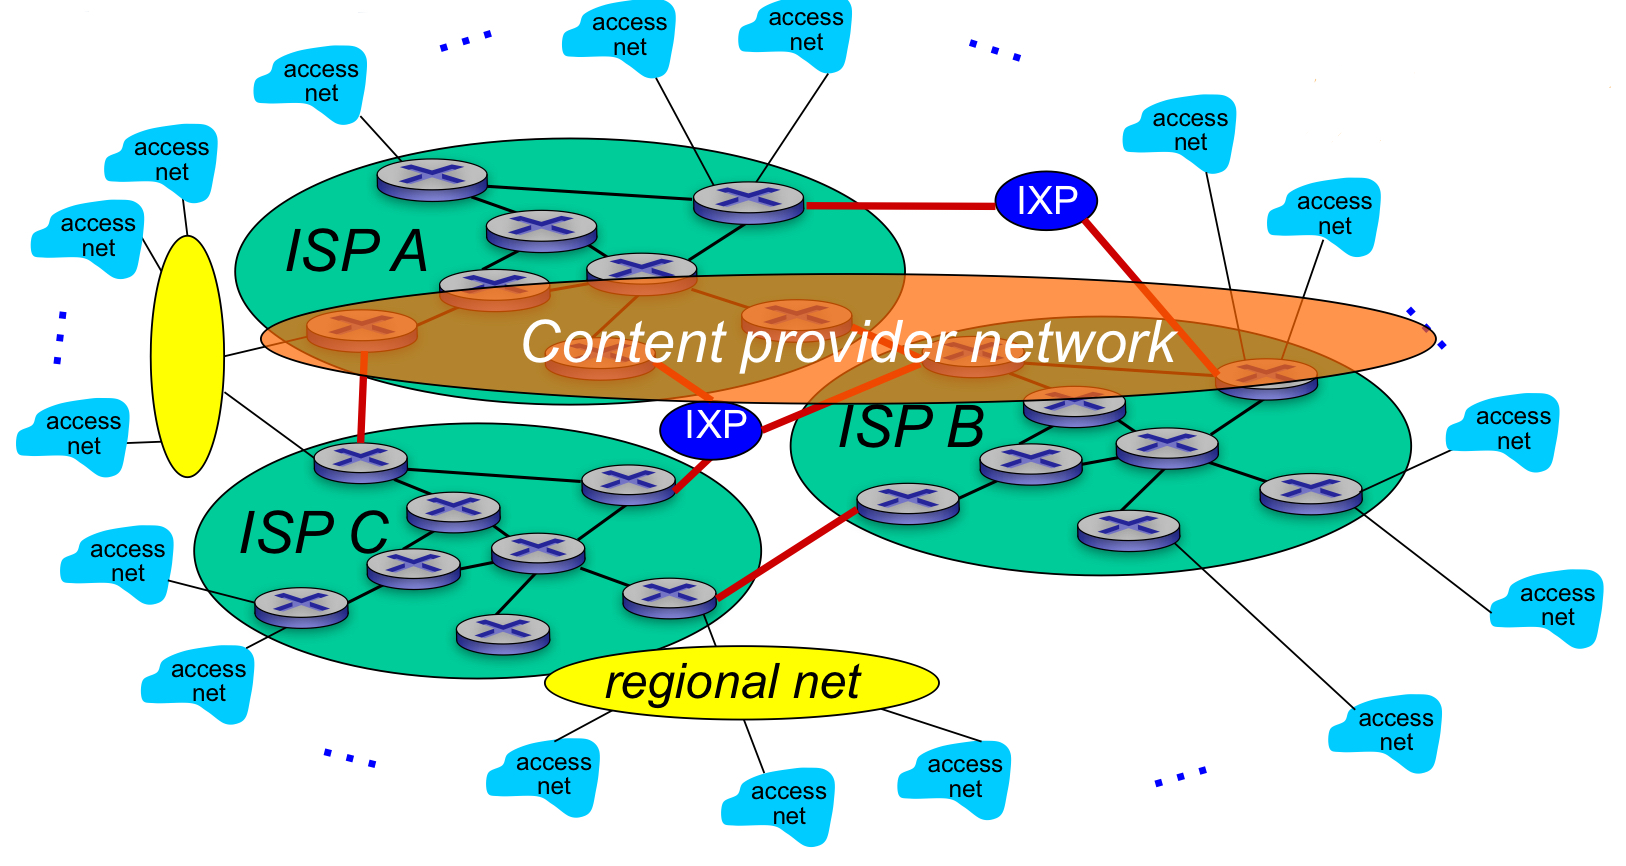
\includegraphics[scale=0.12]{internet}

\begin{itemize}
    \item End systems connect to Internet via \textbf{Access Internet Service Providers (ISPs)} (autonomous systems $\rightarrow$ regional ISP $\rightarrow$ Access ISP $\rightarrow$ hosts)
    \item ISPs connect to larger global ISPs (usually competitors)
    \item Large ISPs connect via \textbf{peering links} or \textbf{internet exchange points (IXP)}
    \item \keyword{IXP}{Physical place with routers from different ISPs}
    \item \keyword{Regional Networks}{Smallers ISPs}
    \item \keyword{Content Provider Networks}{Provide content close to end users}
\end{itemize}

\subsection{Loss, Delay, and Throughput}

\subsubsection{Packet Loss}

\begin{itemize}
    \item If Arrival Rate $>$ Transmission Rate, packets will queue and can be dropped if buffer fills up
    \item Solutions: Lost packets can be retransmitted
\end{itemize}

\subsubsection{Packet Delay}

\[d_{\text{nodal}} = d_{\text{proc}} + d_{\text{queue}} + d_{\text{trans}} + d_{\text{prop}}\]

\begin{itemize}
    \item \keyword{Nodal Processing}{($d_{\text{proc}}$) Check for bit errors and determine output link}
    \item \keyword{Queueing Delay}{($d_{\text{queue}}$) Time at queue waiting for transmission, router congestion}
    \item \keyword{Transmission Delay}{($d_{\text{trans}}$) Time to load packet onto link}
    \begin{itemize}
        \item $d_{\text{trans}} = \frac{L}{R}$ where $L$ is packet length and $R$ is link bandwidth
    \end{itemize}
    \item \keyword{Propagation Delay}{($d_{\text{prop}}$) Time for 1 bit to reach end of link}
    \begin{itemize}
        \item $d_{\text{prop}} = \frac{d}{s}$ where $d$ is length of link and $s$ is propagation speed
        \item Does not depend on packet size, number of packets or number of intermediate nodes
    \end{itemize}
\end{itemize}

\subsubsection{Throughput}

\begin{itemize}
    \item Rate at which bits transferred between hosts
    \begin{itemize}
        \item Different from transmission rate (Theoretical upper bound)
        \item Measures end-to-end, even through intermediaries
        \item Irregardless of the size of packets
        \item Dealing with bottlenecks over n packets:
    \end{itemize}
\end{itemize}
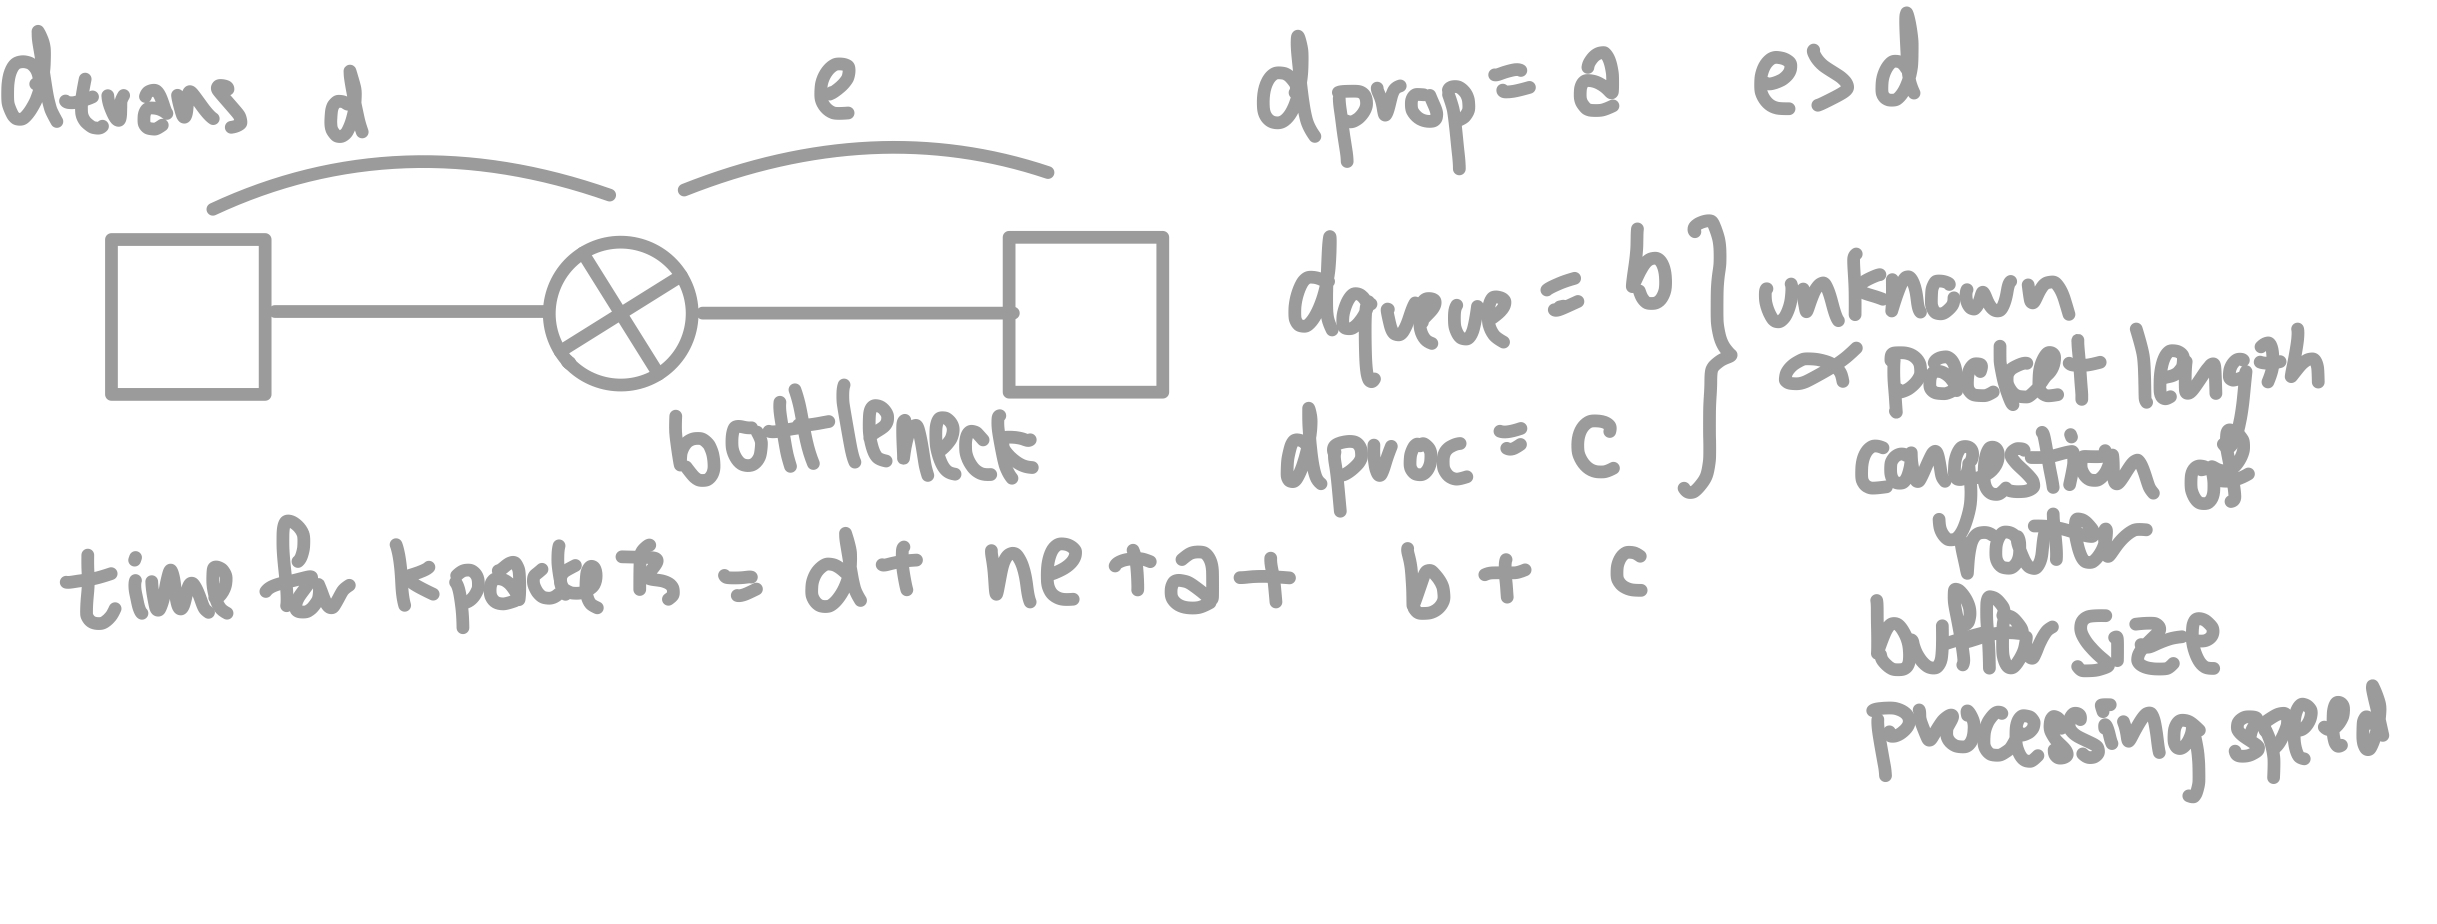
\includegraphics[scale=0.08]{bottleneck}
\begin{itemize}
    \item Average: Rate over long period of time
    \item Instantaneous: Rate at given point in time
\end{itemize}

\subsection{Protocol Layers and Service Models}

\begin{itemize}
    \item \keyword{Protocol}{Defines format, order of messages sent and received, and actions taken on message transmission}
    \item \keyword{Layering}{Each layer implements a service by doing something within layer and relying on services provided by layer below it}
    \begin{itemize}
        \item Explicit structure allows us to make sense of complex components
        \item Easy maintenance (Like OOP, change in 1 layer should not affect others)
    \end{itemize}
\end{itemize}

\subsubsection{Internet Protocol Stack}

\begin{enumerate}
    \item \keyword{Application}{eg. FTP, SMTP}
    \item \keyword{Transport}{TCP, UDP}
    \item \keyword{Network}{IP, Routing protocols}
    \item \keyword{Link}{Ethernet, WiFi, PPP}
    \item \keyword{Physical}{Wires, bits}
\end{enumerate}
\keyword{Encapsulation} Take information from a higher layer and adds a header to it, treating the higher layer information as data

\subsection{Topology}
	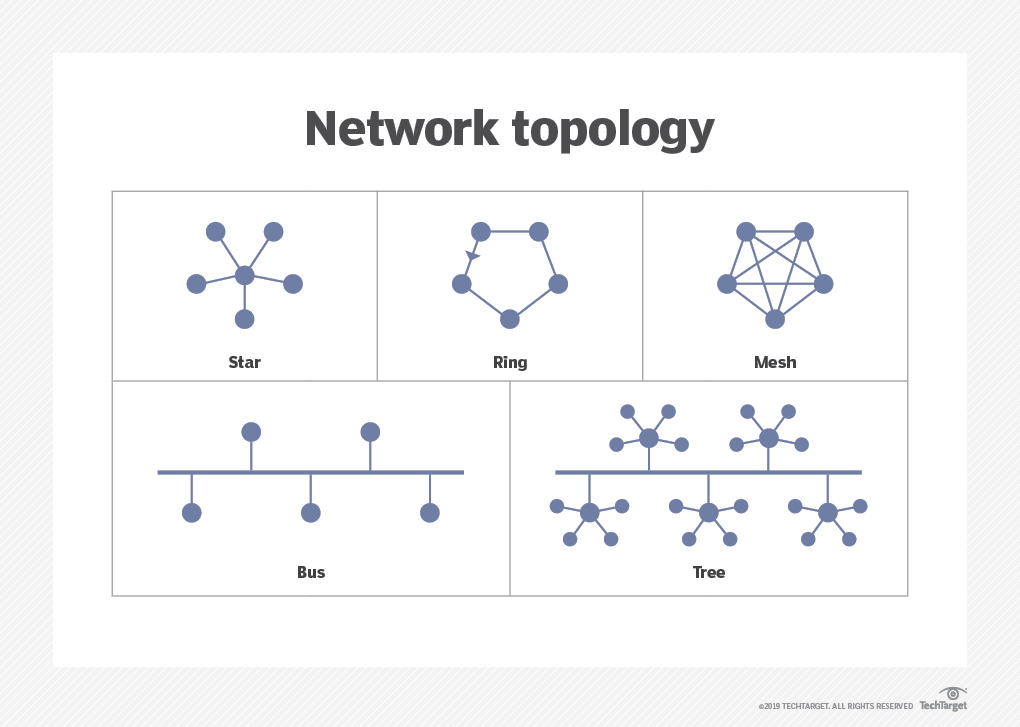
\includegraphics[scale=0.19]{topology}
	\begin{itemize}
		\item \keyword{Star}{Lowest cost and simplest}
		\item \keyword{Mesh}{High redundancy, increased cost but highest transmission speeds}
	\end{itemize}
	
% -----------------------------------------------------------------------
\section{02. Application Layer}

\begin{itemize}
    \item Programs that run on end systems, and not on network-core devices
\end{itemize}

\subsection{Client-server Architecture}

\begin{itemize}
    \item Server: Always-on host, Permanent IP address, waits for incoming req and provides service to client
    \item Clients: Communicates with server, Intermittently connected, Dynamic IP addresses, Do not communicate with each other directly, initate connection with server to request services
\end{itemize}

\subsection{P2P Architecture}

\begin{itemize}
    \item Peers request service from other peers and provide service in return
    \item No always-on server, Intermittently connected, Dynamic IP addresses
    \item \keyword{Self Scalability}{New peers offer new services and demands}
\end{itemize}

\subsection{Process}

\begin{itemize}
    \item \keyword{Inter-process Communication}{How 2 processes in 1 host communicate}
    \item \keyword{Socket}{Process sends/receives messages to/from its socket (like a door)}
    \begin{itemize}
        \item Outside of socket, transport layer delivers message
    \end{itemize}
\end{itemize}

\subsection{Addressing Processes}

\begin{itemize}
    \item Motivation: IP address is not enough to address process, since many processes can be running on same host
    \begin{itemize}
        \item \keyword{Identifier}{IP address and port number}
        \item \keyword{IP}{32-bit address for identifying host}
        \item \keyword{Port Number}{16-bit to identify specific process on host}
    \end{itemize}
\end{itemize}

\subsection{Services}
\begin{itemize}
	\item \keyword{Data Integrity}{Reliable data transfer}
	\item \keyword{Timing}{Low delay/latency}
	\item \keyword{Throughput}{Minimum amount of throughput for effectiveness}
	\item \keyword{Security}{Encryption, data integrity}
\end{itemize}

\subsection{Transport Protocol Services}

\begin{enumerate}
    \item \keyword{TCP}{Transmission Control Protocol}
    \begin{itemize}
        \item Reliable transport
        \item Flow control: Sender does not overwhelm receiver
        \item Congestion control
        \item Connection-oriented: Setup required between client and server
    \end{itemize}
    \item \keyword{UDP}{User Datagram Protocol}
    \begin{itemize}
        \item Unreliable data transfer
        \item Fast
    \end{itemize}
\end{enumerate}
\begin{itemize}
	\item Does not guarantee minimum throughput and timing
\end{itemize}

\subsection{App-layer Protocol}

\begin{itemize}
    \item Types of messages exchanged (e.g. Request or response)
    \item Message syntax: How fields are delineated
    \item Messages semantics: Meaning of information in fields
\end{itemize}

\subsection{HTTP - 80}

\begin{itemize}
    \item \keyword{Hypertext Transfer Protocol}{Web's application layer protocol}
    \item Motivation: Web page consists of objects (HTML, images). Need method to request/send web objects.
    \item Follows client/server model
    \item Uses TCP
    \item \keyword{Stateless}{Server maintains no information about past requests}
\end{itemize}

\subsubsection{Non-persistent HTTP 1.0}

\begin{itemize}
    \item At most 1 object sent over TCP connection
    \item Downloading multiple objects requires multiple TCP connections
    \item New TCP connection for each web resource/object
\end{itemize}

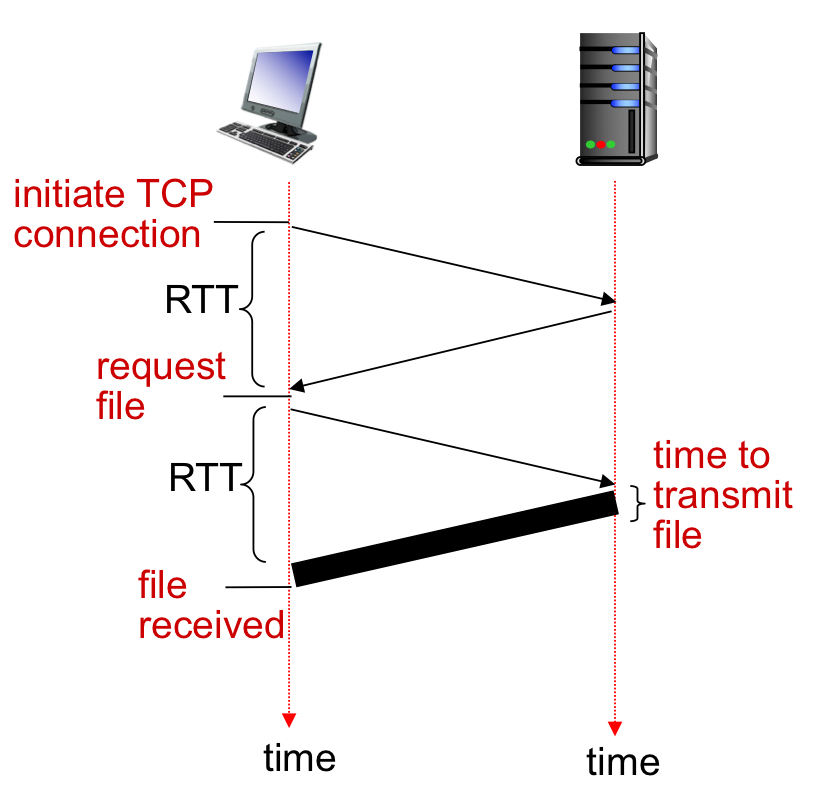
\includegraphics[scale=0.15]{non-persistent-http}

\begin{itemize}
    \item Server closes TCP connection after sending file
    \item \keyword{Return Trip Time}{(RTT) Time for small packet to travel from client to server and back}
    \item RTT is $2*d_{prop}$
    \item Response Time: 2 RTT + File transmission time
\end{itemize}
\end{multicols*}
\begin{multicols*}{3}
\subsubsection{Persistent HTTP}

\begin{itemize}
    \item Multiple objects can be sent over single TCP connection
    \item Server leaves TCP connection open after sending response
    \item As little as one RTT for all referenced objects
\end{itemize}

\subsubsection{HTTP Request Message}

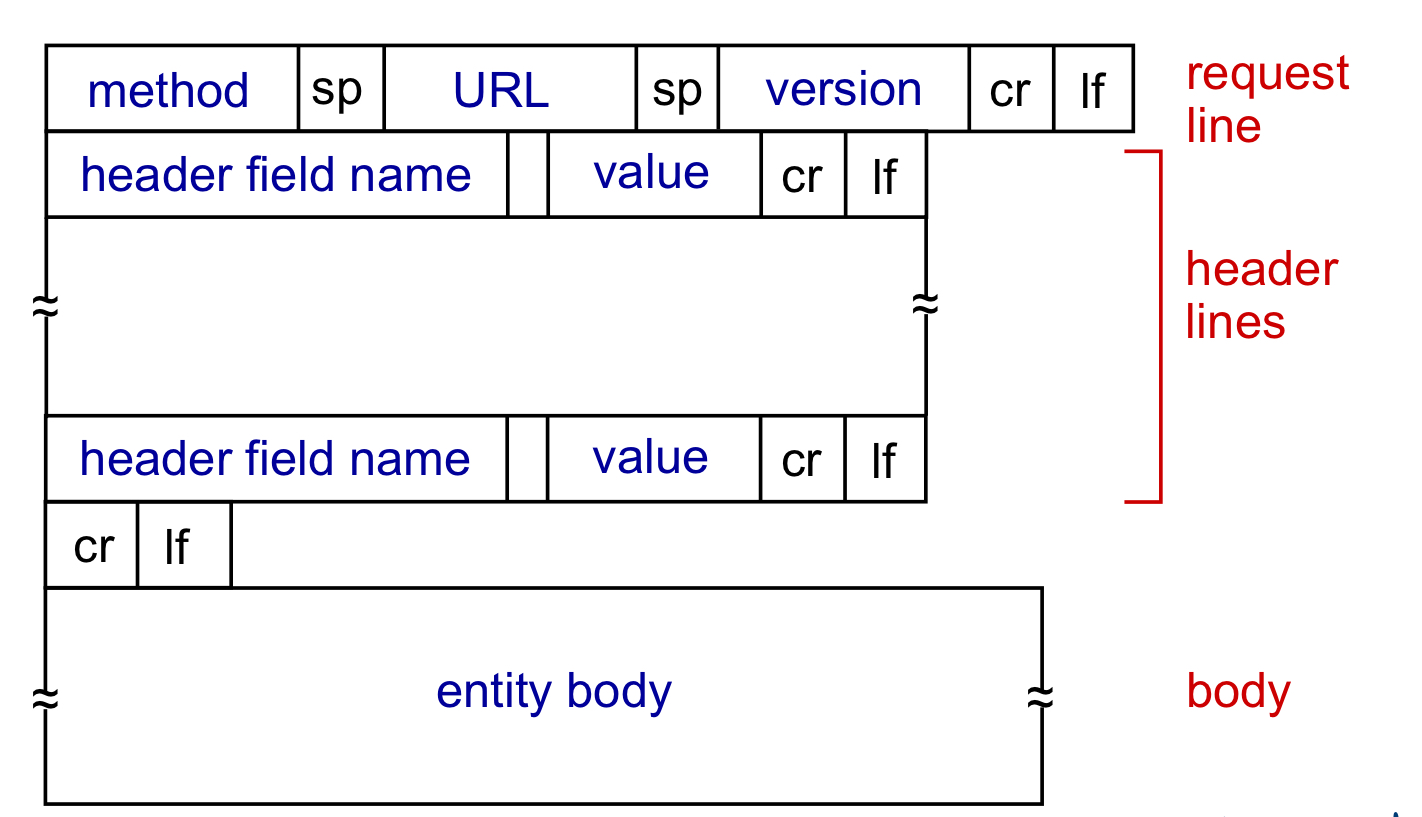
\includegraphics[scale=0.14]{http-request}

\begin{itemize}
    \item To upload form input: \keyword{POST method}{Input uploaded via entity body} and \keyword{URL method}{Input uploaded in URL field of GET method}
    \item \keyword{HTTP/1.0}{GET, POST, HEAD (Ask server to leave request object out of response)}
    \item \keyword{HTTP/1.1}{GET, POST, HEAD, PUT, DELETE}
\end{itemize}

\subsubsection{HTTP Response Message}

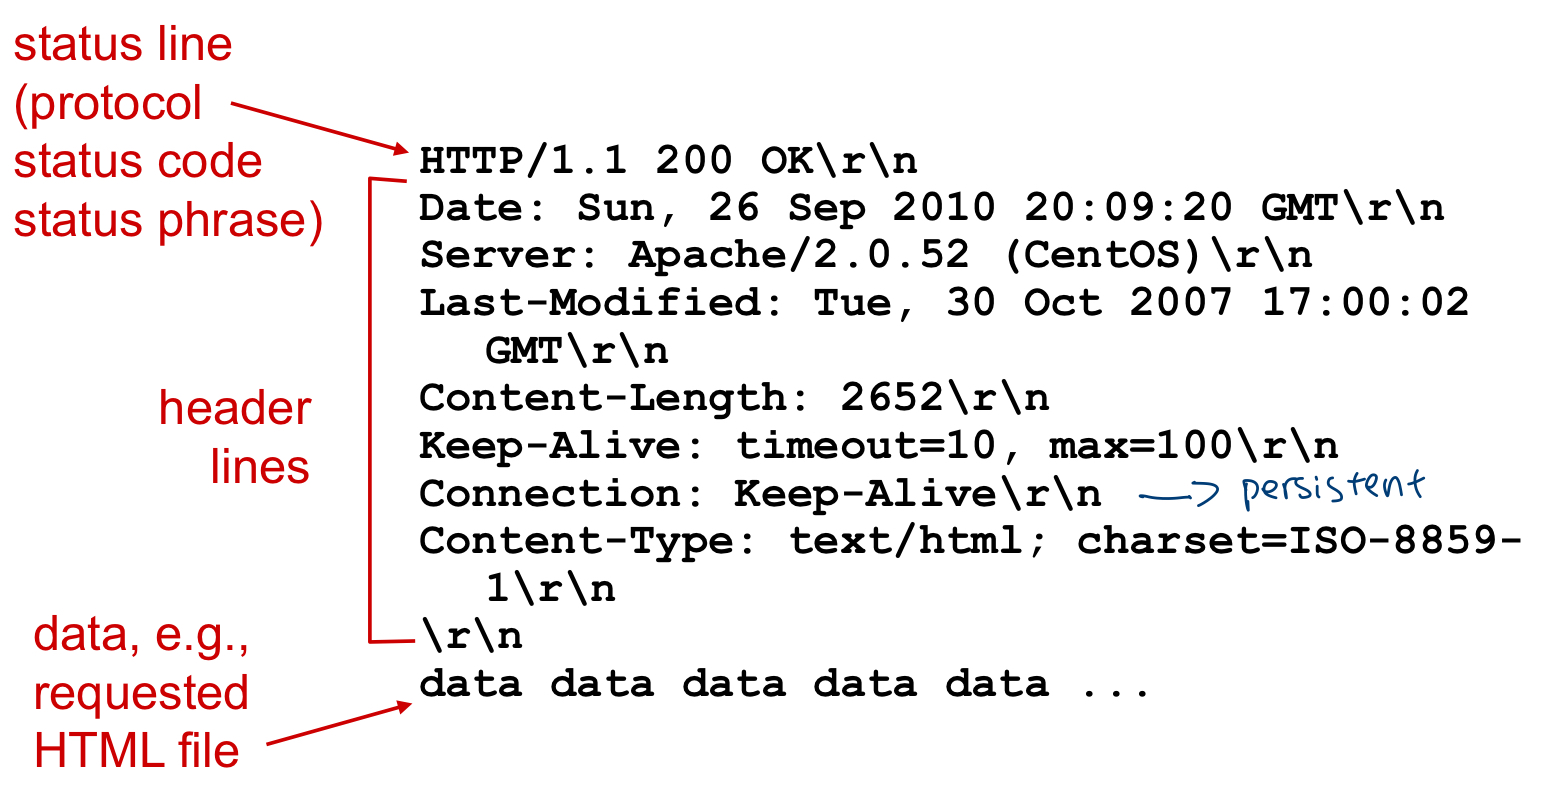
\includegraphics[scale=0.12]{http-response}


\subsubsection{Error codes}
\begin{description}
	\item[200]{OK}
	\item[301]{Moved permanently}
	\item[304]{Not modified (during conditional GET)}
	\item[400]{Bad request}
	\item[404]{Resource not found}
	\item[505]{HTTP Version Not Supported}
\end{description}


\subsubsection{Cookies}

\begin{itemize}
    \item Maintains state on client side
    \item Components: Cookie header for HTTP response, Cookie header for HTTP, request, Cookie file on user's host (Key-value pair), Database on server
\end{itemize}

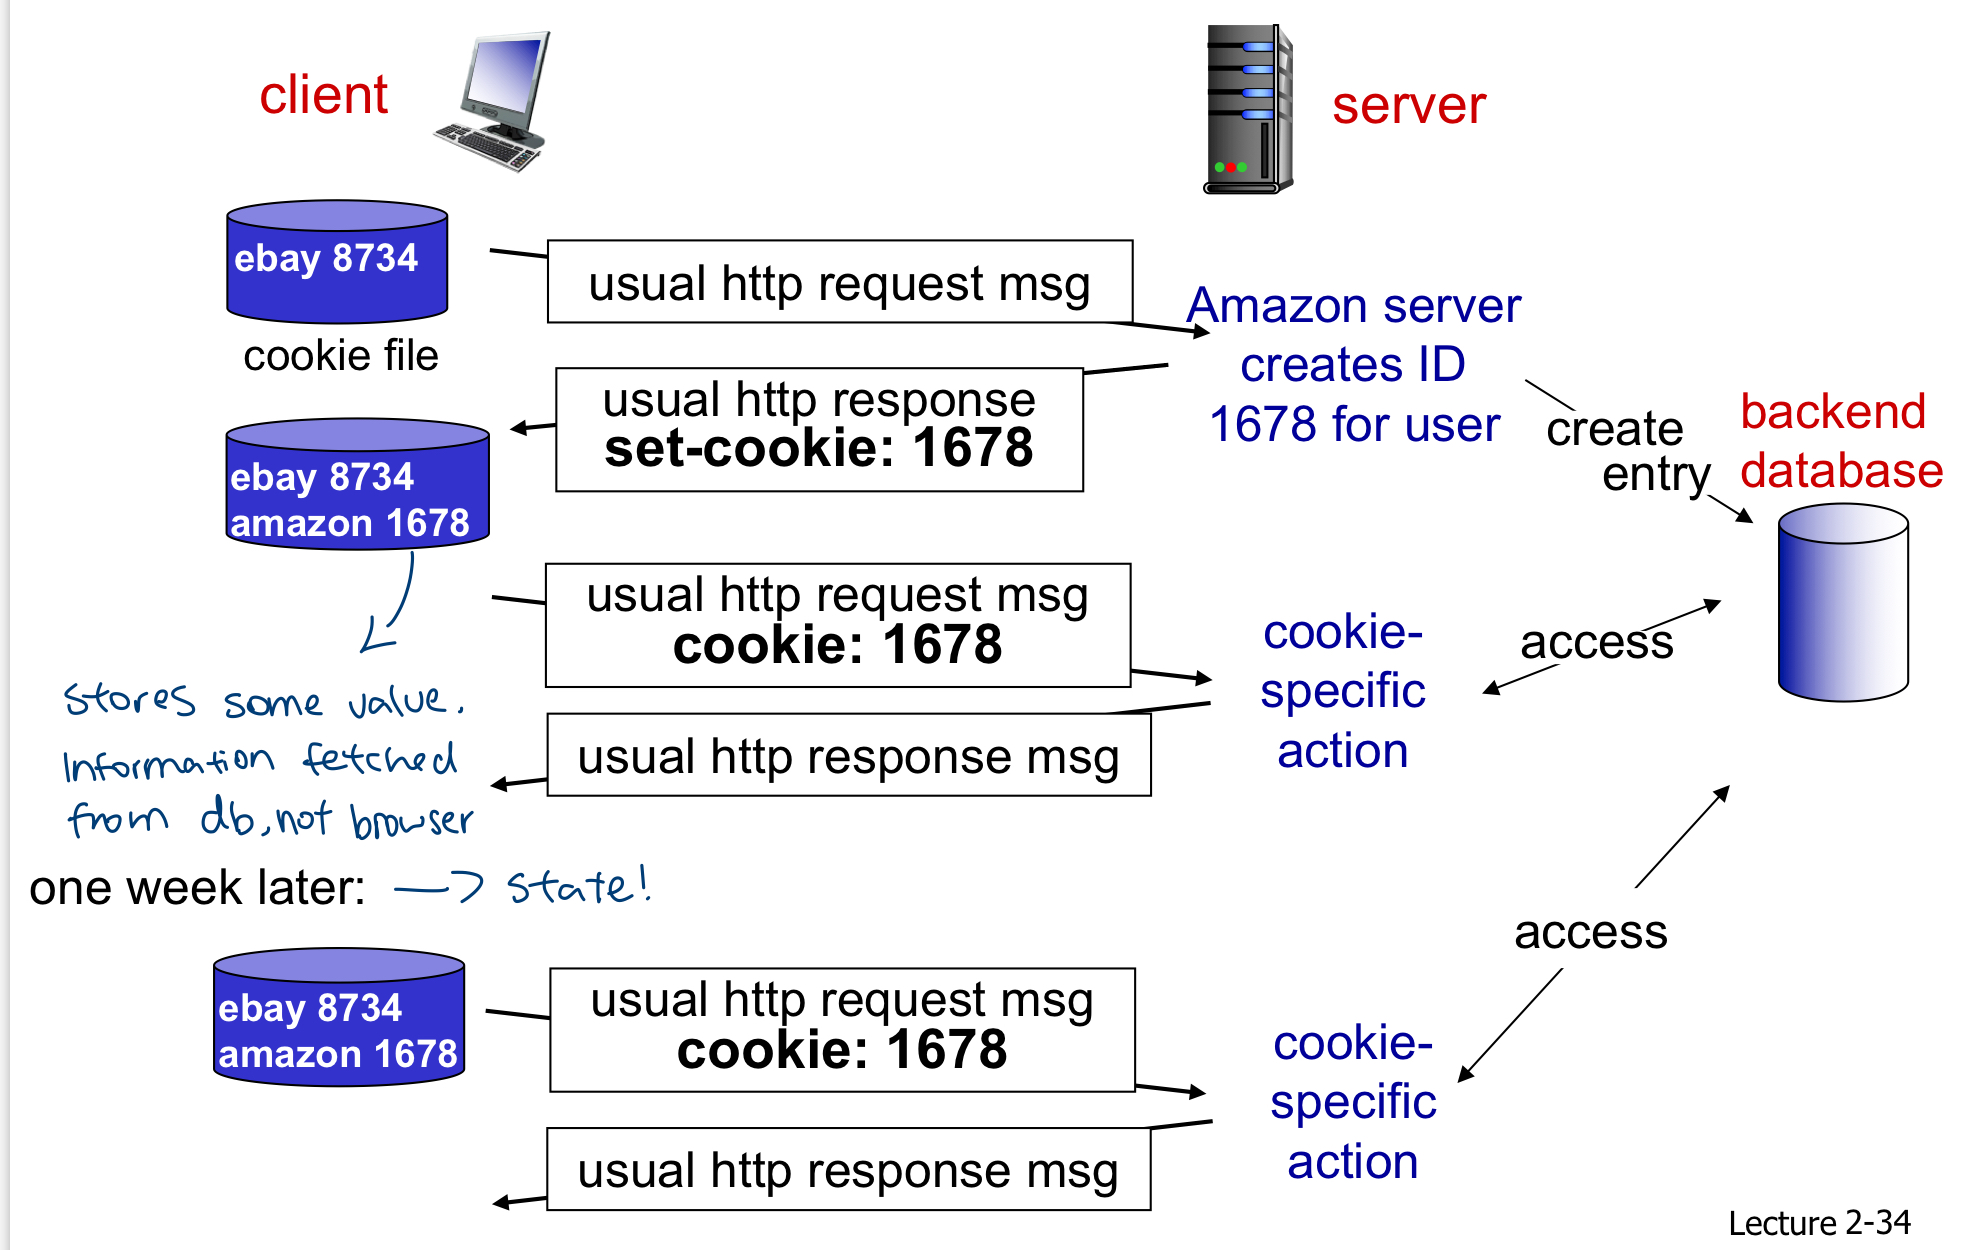
\includegraphics[scale=0.1]{cookies}


\subsubsection{Web Cache (Proxy Server)}

\begin{itemize}
    \item Goal: Fulfill request without involving origin server via caching
    \item Browser sends all HTTP requests to cache
    \item Pros: Faster, Reduces traffic to origin server
    \item Cons: What if origin server updates?
    \begin{itemize}
        \item \keyword{Conditional GET}{Origin server doesn't send object if cache has updated version}
        \item Cache: Specifies date of cached copy in HTTP request to origin (If-modified-since)
        \item Origin Server: Response contains no object if cached object is updated (Empty content body)
    \end{itemize}
\end{itemize}

\subsection{Domain Name System - 53}

\begin{itemize}
    \item Maps between hostname (e.g. yahoo.com) and IP address
    \item Implemented using distributed and hierarchical databases
    \item Application-layer protocol (Why?)
    \begin{tabbing}
    	\= Build complexity in edges to simplify inner core networks
    \end{tabbing}
    \item Uses UDP (Much faster and smaller packet overhead)
    \item Services provided
    \begin{description}
    	\item[Host/Email aliasing] {Additional name for complicated hostnames}
    	\item[Load balancing] {Providing multiple IP addresses for the same URL}
    \end{description}
    \item \keyword{Local DNS Name Server}{Local cache of name-to-address mapping. Forwards query into hierarchy.}
    \begin{itemize}
        \item \keyword{Time to Live}{(TTL) Cached mappings disappear after some time}
    \end{itemize}
    \item \keyword{Root Name Server}{Contacted by local name server that cannot resolve name. Provides IP address of TLD servers.}
    \item \keyword{Top-level Domain Server}{(TLD) Provides IP address of authoritative server}
    \item \keyword{Authoritative DNS Server}{Organization's own DNS server. Provides mappings for organization's named hosts.}
\end{itemize}

\begin{itemize}
	\item Iterated query: "Not sure, ask this server"    
\end{itemize}
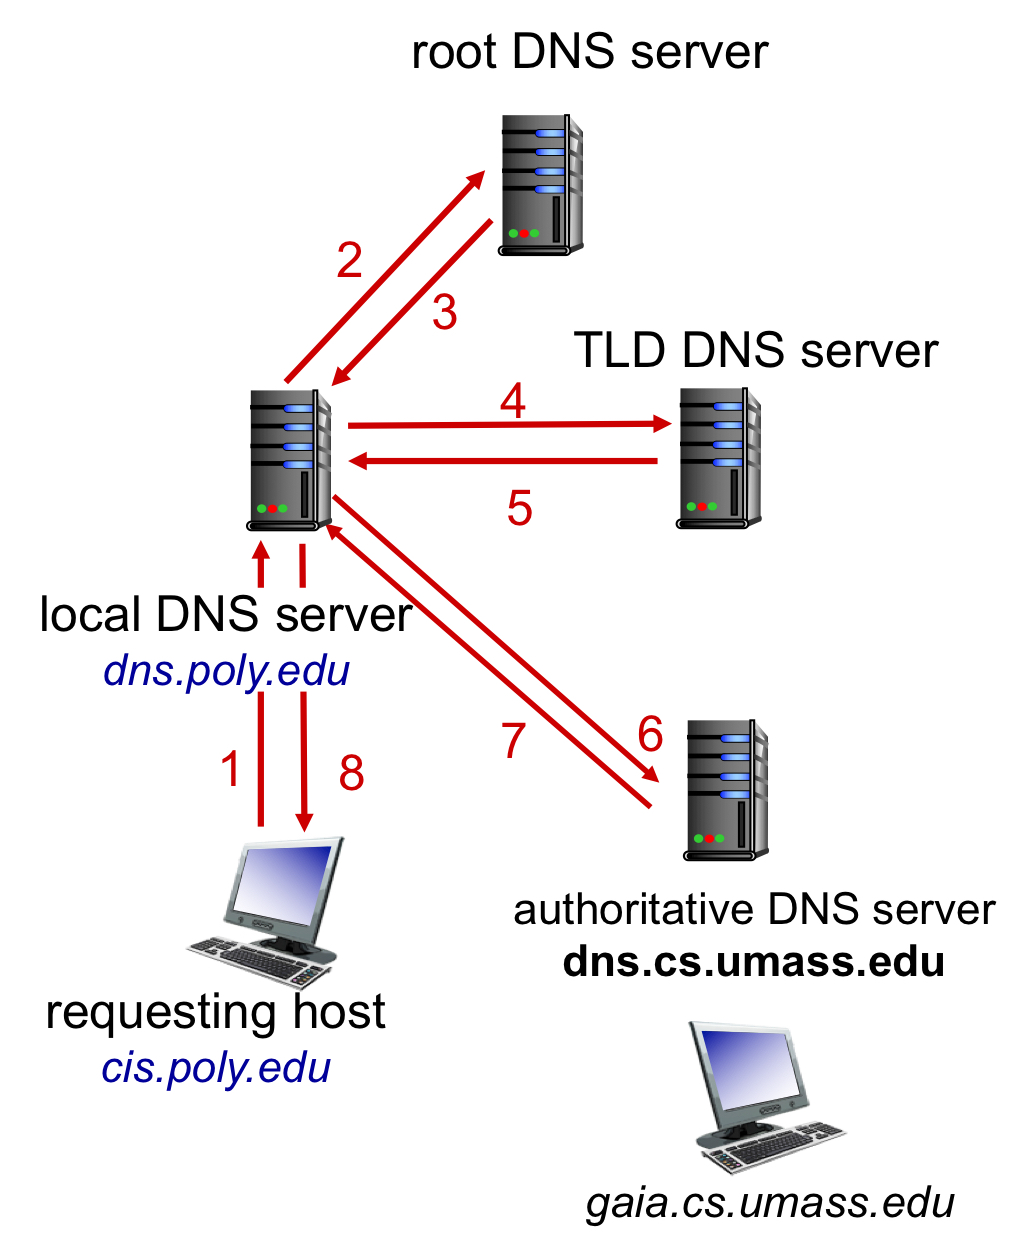
\includegraphics[scale=0.08]{dns-iterative-query}
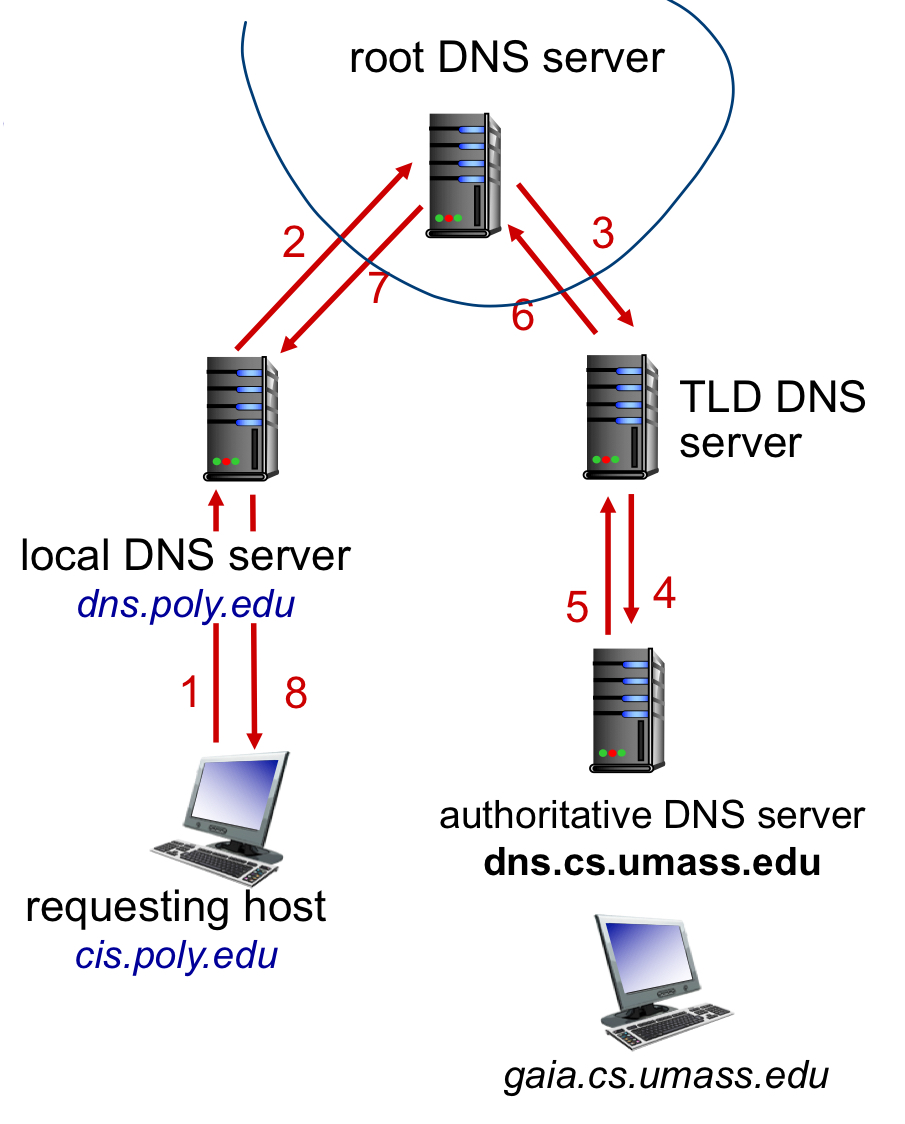
\includegraphics[scale=0.1]{dns-recursive-query}
\begin{itemize}
    \item Recursive query: "Okay, let me find for you"
    \begin{itemize}
        \item Heavy load on upper levels of hierarchy
    \end{itemize}
\end{itemize}
Local DNS servers does both


\subsection{DNS Caching}
\keyword{Cache entry}{Cache record of recent name mapping}

\begin{itemize}
	\item Timeout after some time based on TTL
	\item Best effort name-to-address translation (can be out-of-date)
	\item \keyword{Resource record}{Mapping btw hostname and IP}
	\item Format: <NAME, TYPE, VALUE, TTL>
\end{itemize}
\subsubsection{DNS Cache poisoning}
\begin{itemize}
	\item DNS spoofing attack - Rogue DNS records introduced in resolver's cache, leading to incorrect IP address reply
\end{itemize}

% -----------------------------------------------------------------------
\section{03. Socket Programming with UDP and TCP}

\subsection{UDP Socket}

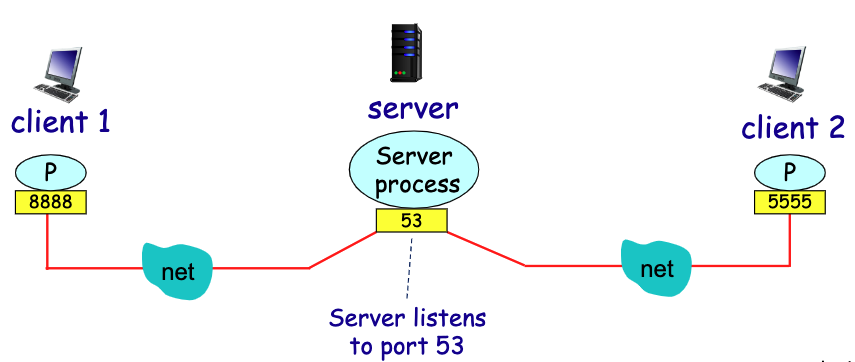
\includegraphics[scale=0.17]{udp-socket}\\
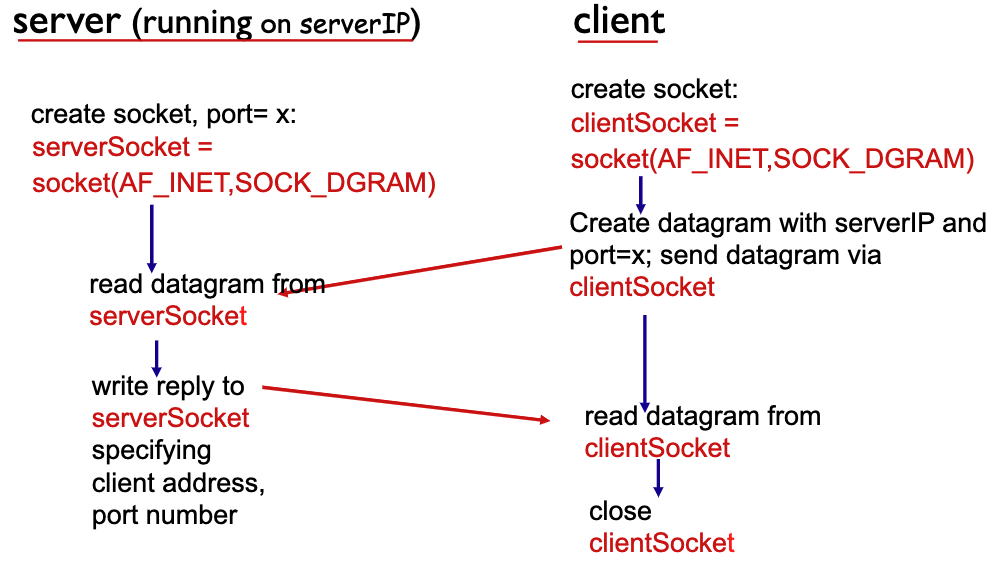
\includegraphics[scale=0.18]{udp}

\begin{itemize}
    \item No connection beforehand. Just send it.
    \item Server has 1 socket to serve all clients
    \item Sender attaches destination IP address and port number (\textbf{Stateless})
    \item Unreliable datagram: Data may be lost or out-of-order
    \begin{itemize}
        \item \keyword{Datagram}{Group of bytes}
    \end{itemize}
\end{itemize}
\subsection{TCP Socket}

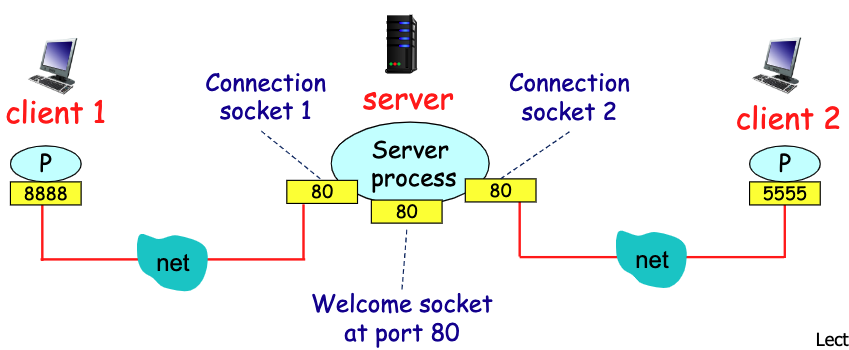
\includegraphics[scale=0.3]{tcp-socket}\\
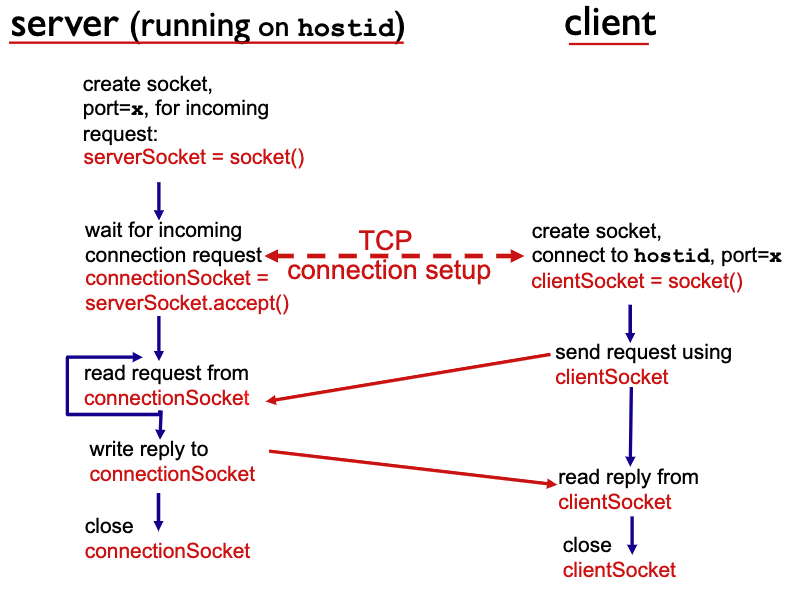
\includegraphics[scale=0.35]{tcp}

\begin{itemize}
    \item Client establishes connection to server via welcome socket
    \item Server makes new socket for each client
    \item Server identifies client via connection (\textbf{Stateful})
    \item Reliable stream pipe: Data always in order
\end{itemize}

\subsection{Remarks}
\begin{itemize}
	\item SOCK\_STREAM - TCP, SOCK\_DGRAM - UDP
	\item Can only specify destination port numbers, source port numbers randomly assigned by OS
\end{itemize}

% -----------------------------------------------------------------------

\section{04. UDP and Reliable Protocol}

\subsection{Transport Layer Services}
\begin{itemize}
	\item Provide logical communication between processes in different hosts 
	\item VS network: Process-to-process VS host-to-host
	\item Sender: Breaks app messages into segment
	\item Receiver: Reassembles segments
\end{itemize}

\subsection{UDP}

\begin{itemize}
    \item On top of network layer, UDP adds:
    \begin{enumerate}
        \item Connectionless multiplexing/de-multiplexing
        \begin{itemize}
            \item UDP segments contain both source and destination ports
            \item \keyword{Multiplexing}{Sent to target processes}
            \item \keyword{Demultiplexing}{Delivering the received segments at the receiver side to the correct app layer processes}
        \end{itemize}
        \item Checksum
    \end{enumerate}
\end{itemize}

\subsubsection{UDP Segment Header}
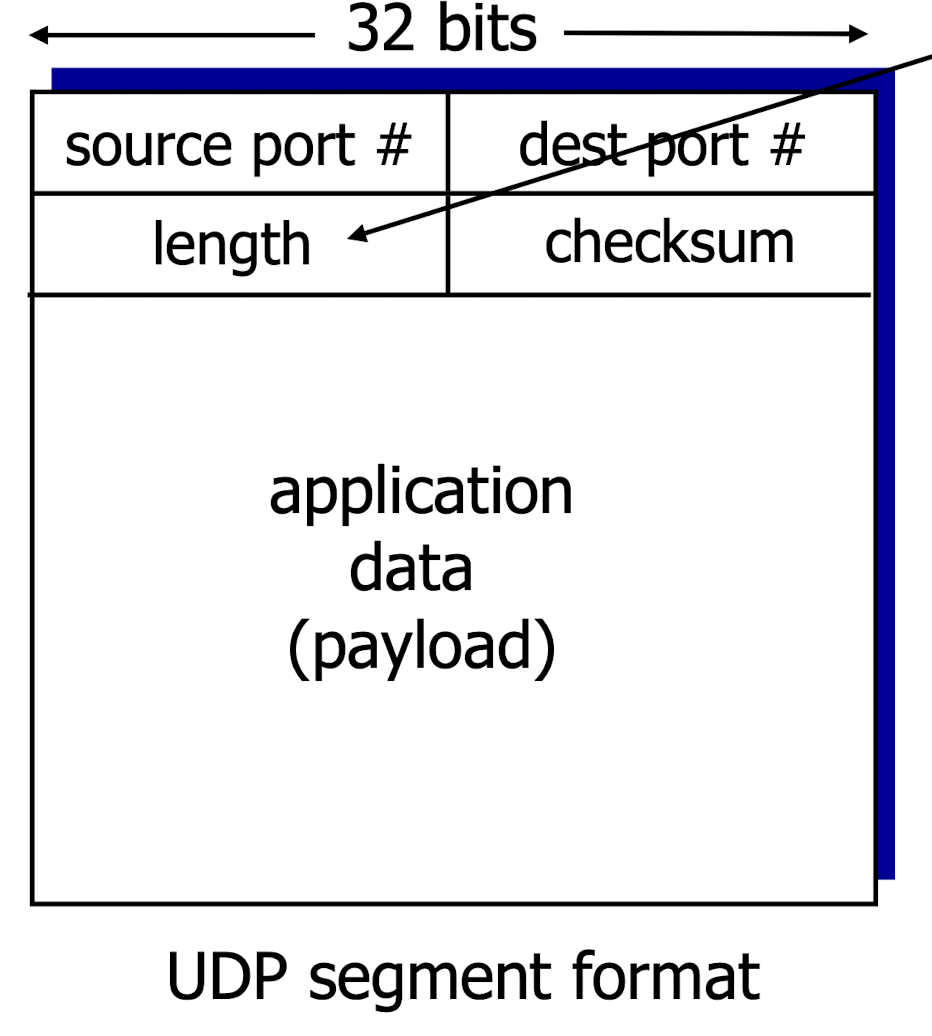
\includegraphics[scale=0.19]{udp-segment-header}
\\Note that length includes 8 byte header + body content

\subsubsection{Checksum}

\begin{itemize}
    \item Goal: Detect errors in received segment
\end{itemize}

\begin{enumerate}
    \item Treat UDP segment as sequence of 16-bit integers
    \item Add every 16-bit integer (Carry added back to result)
    \item Invert to get UDP checksum (1's complement)
    \item When receiving, sum segment again. All 1s if correct.
\end{enumerate}

\subsection{Reliable Data Transfer (rdt)}

\begin{itemize}
    \item Characteristics of unreliable channel will determine services provided by rdt
    \item Cannot fix unordered packets
\end{itemize}

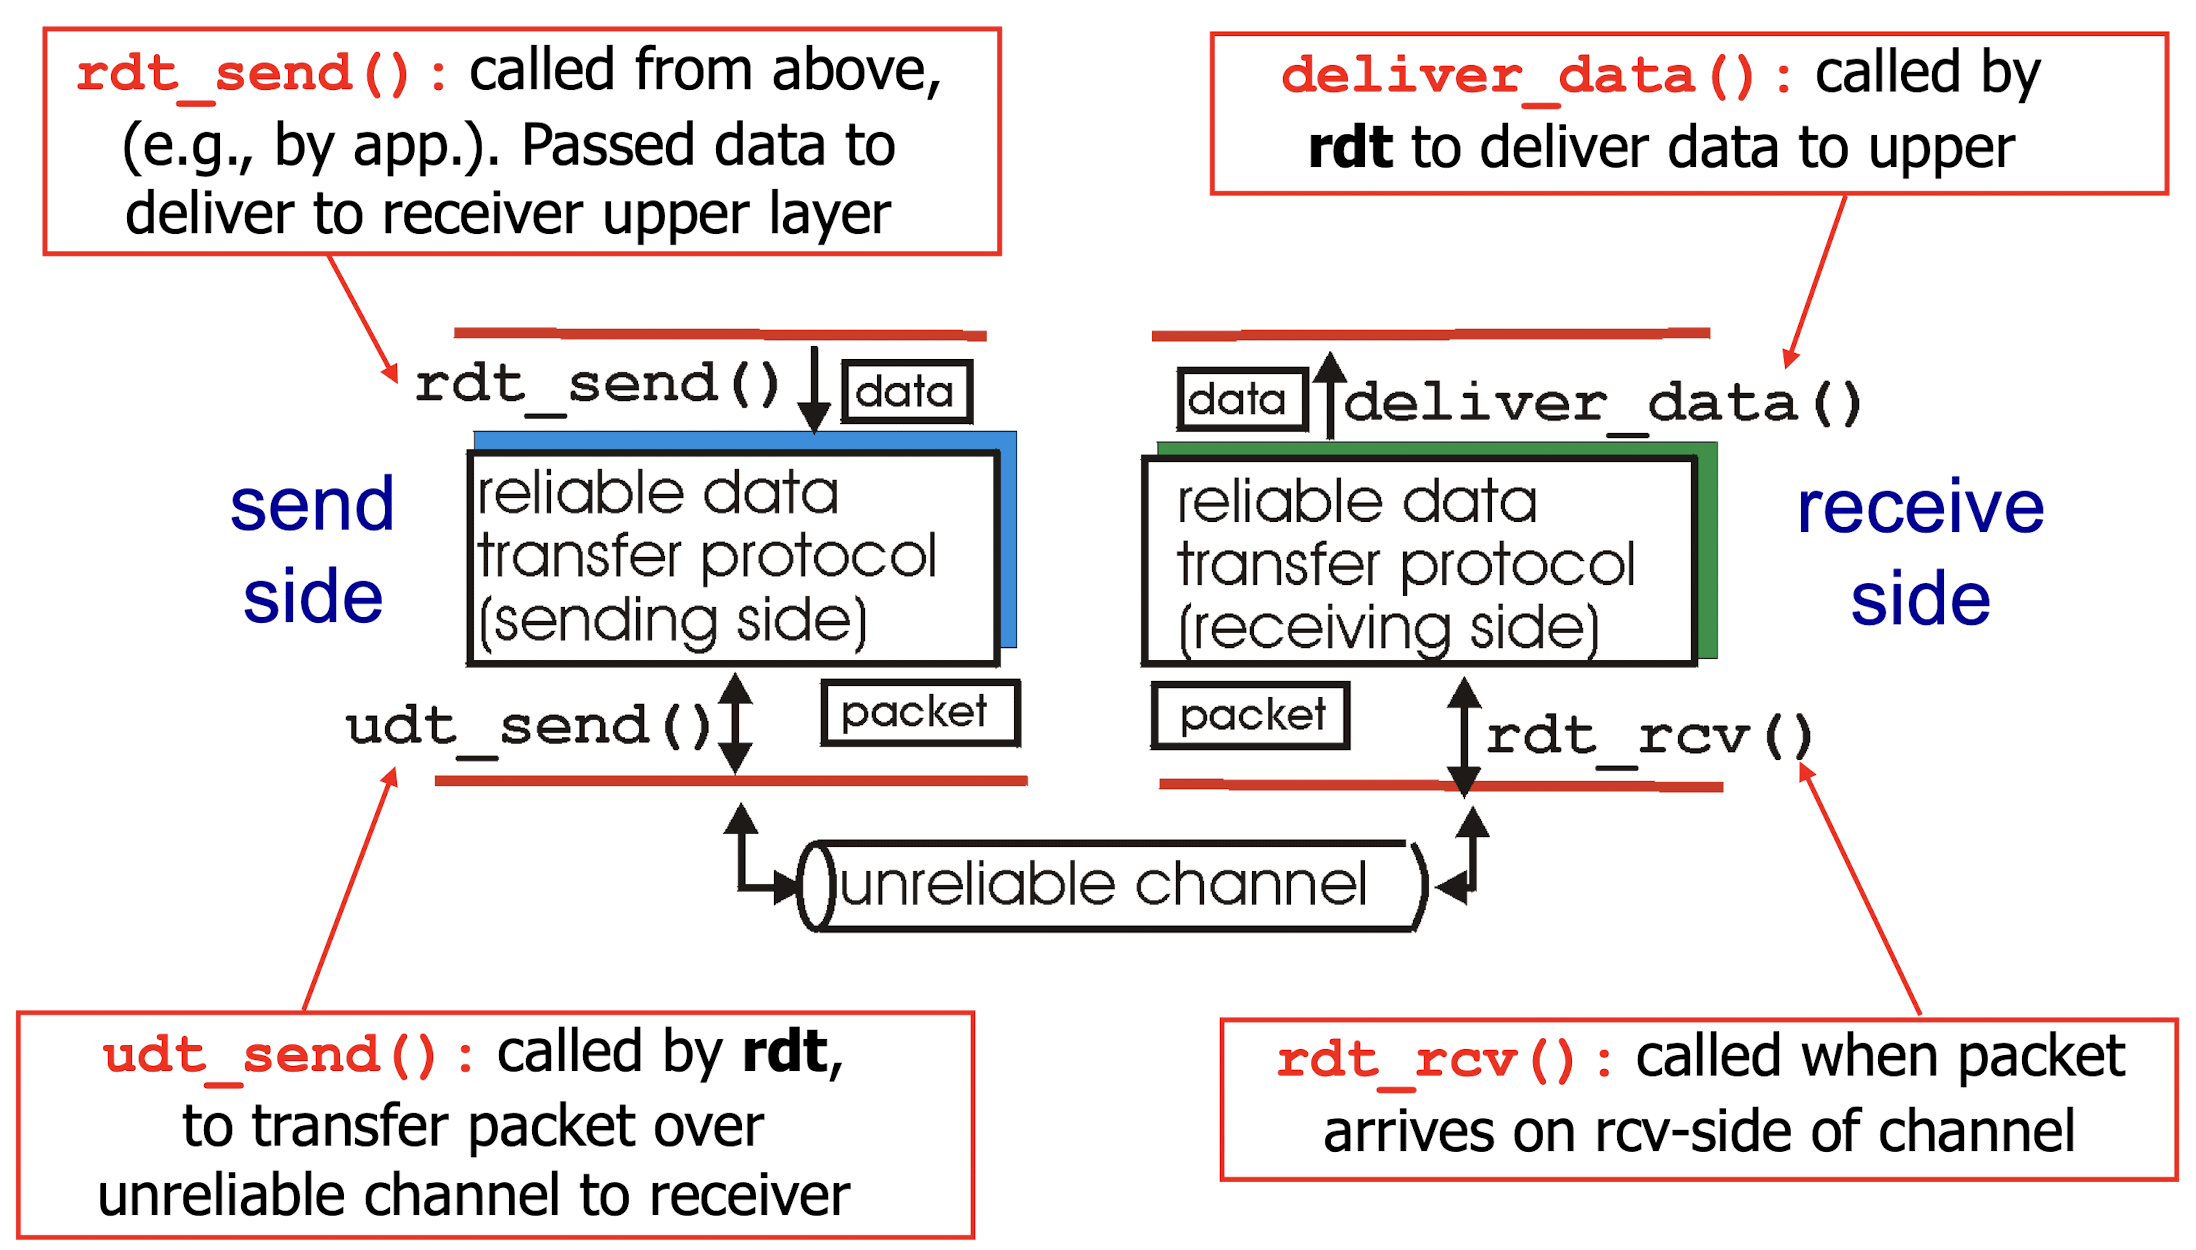
\includegraphics[scale=0.2]{rdt-interfaces}

\subsubsection{rdt 2.0}

\begin{itemize}
    \item New problem: \keyword{Bit error}{May flip bits in packet}
    \item Solution:
    \begin{itemize}
        \item Perform checksum to detect bit errors
        \item \keyword{Stop and wait protocol}{Sender sends one packet at a time and wait for response}
        \item \keyword{ACK}{Receiver tells sender that packet received is ok}
        \item \keyword{NAK}{Receiver tells sender that packet received has errors (retransmission)}
    \end{itemize}
\end{itemize}

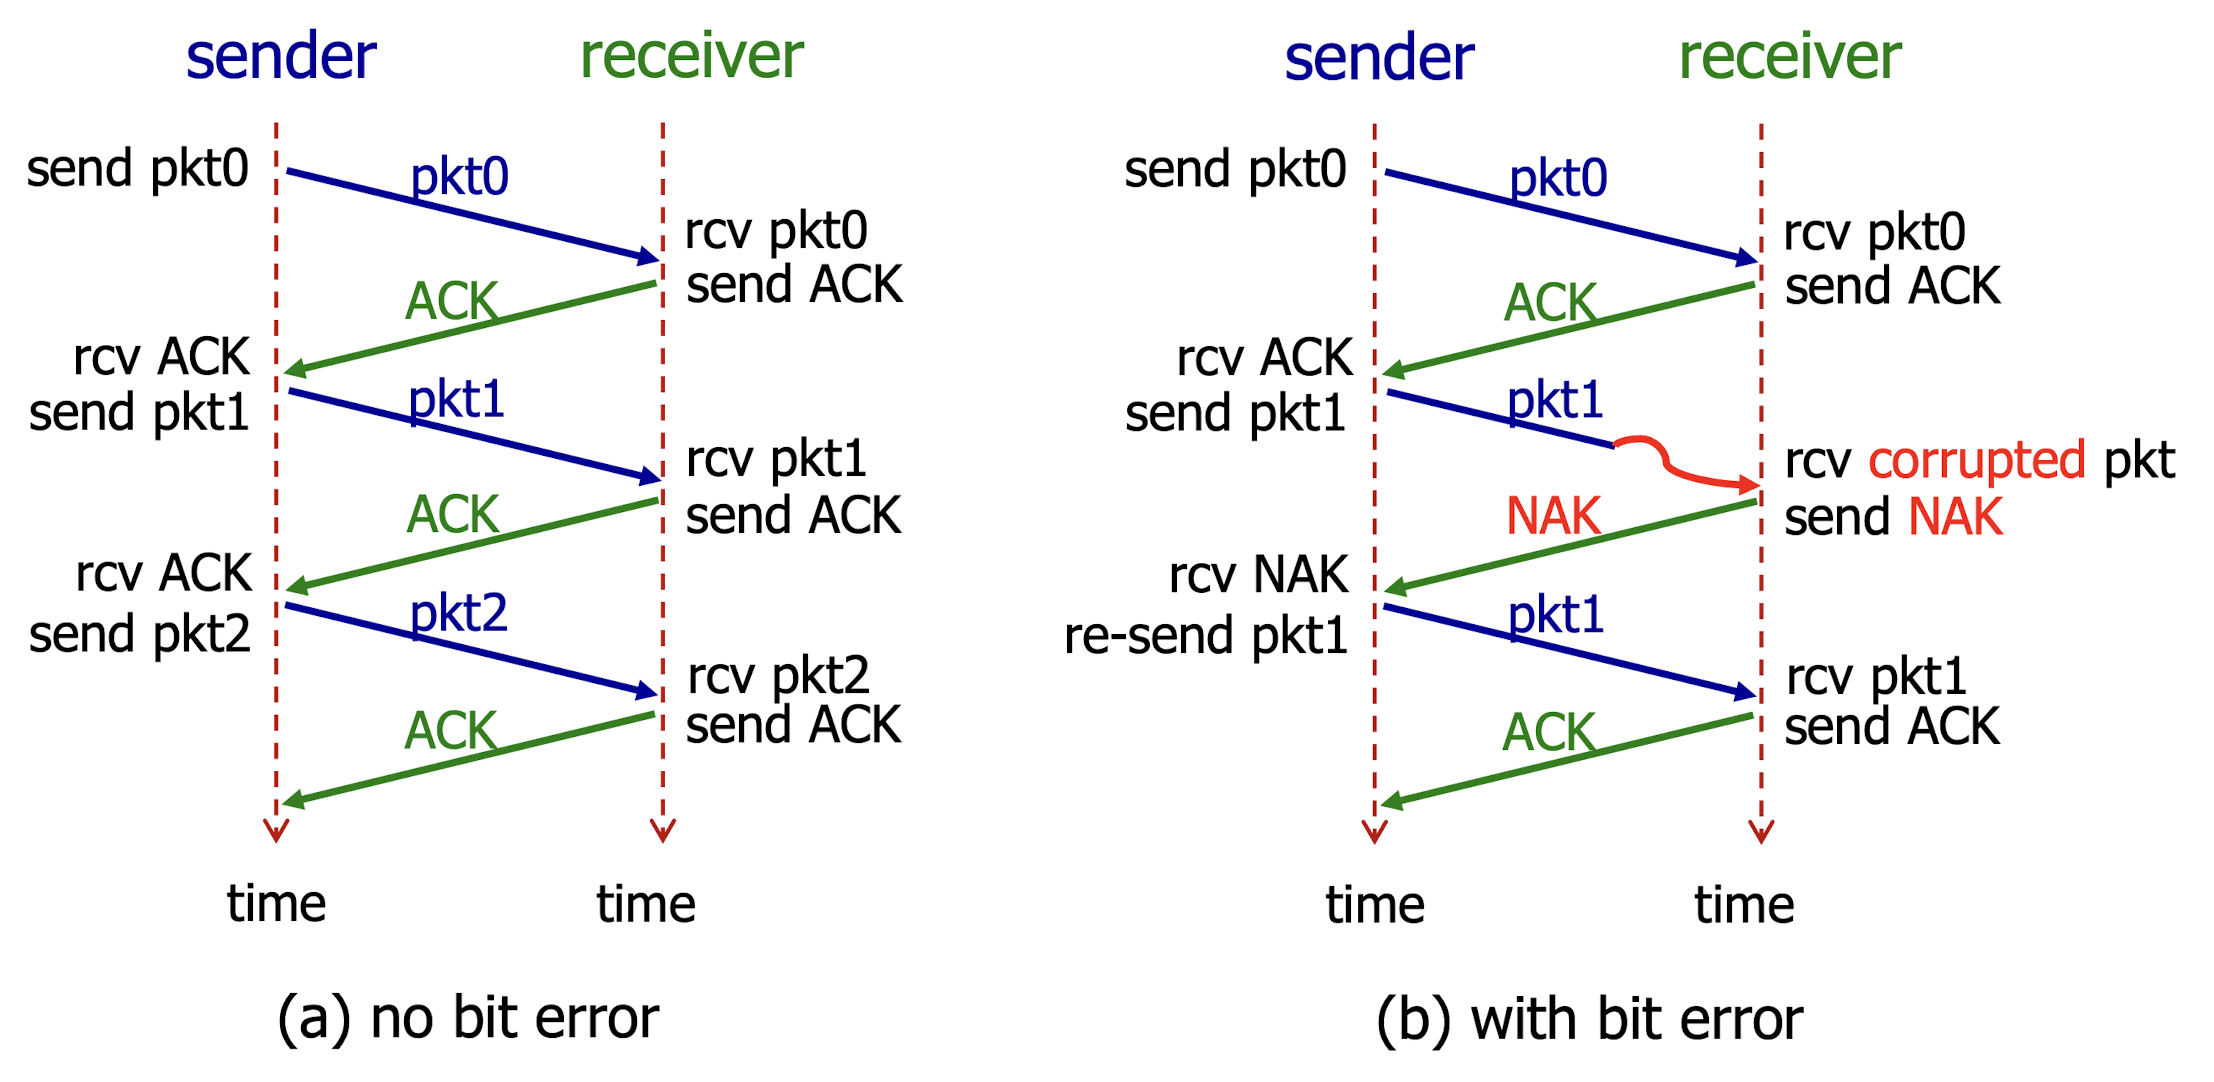
\includegraphics[scale=0.2]{rdt-2.0}

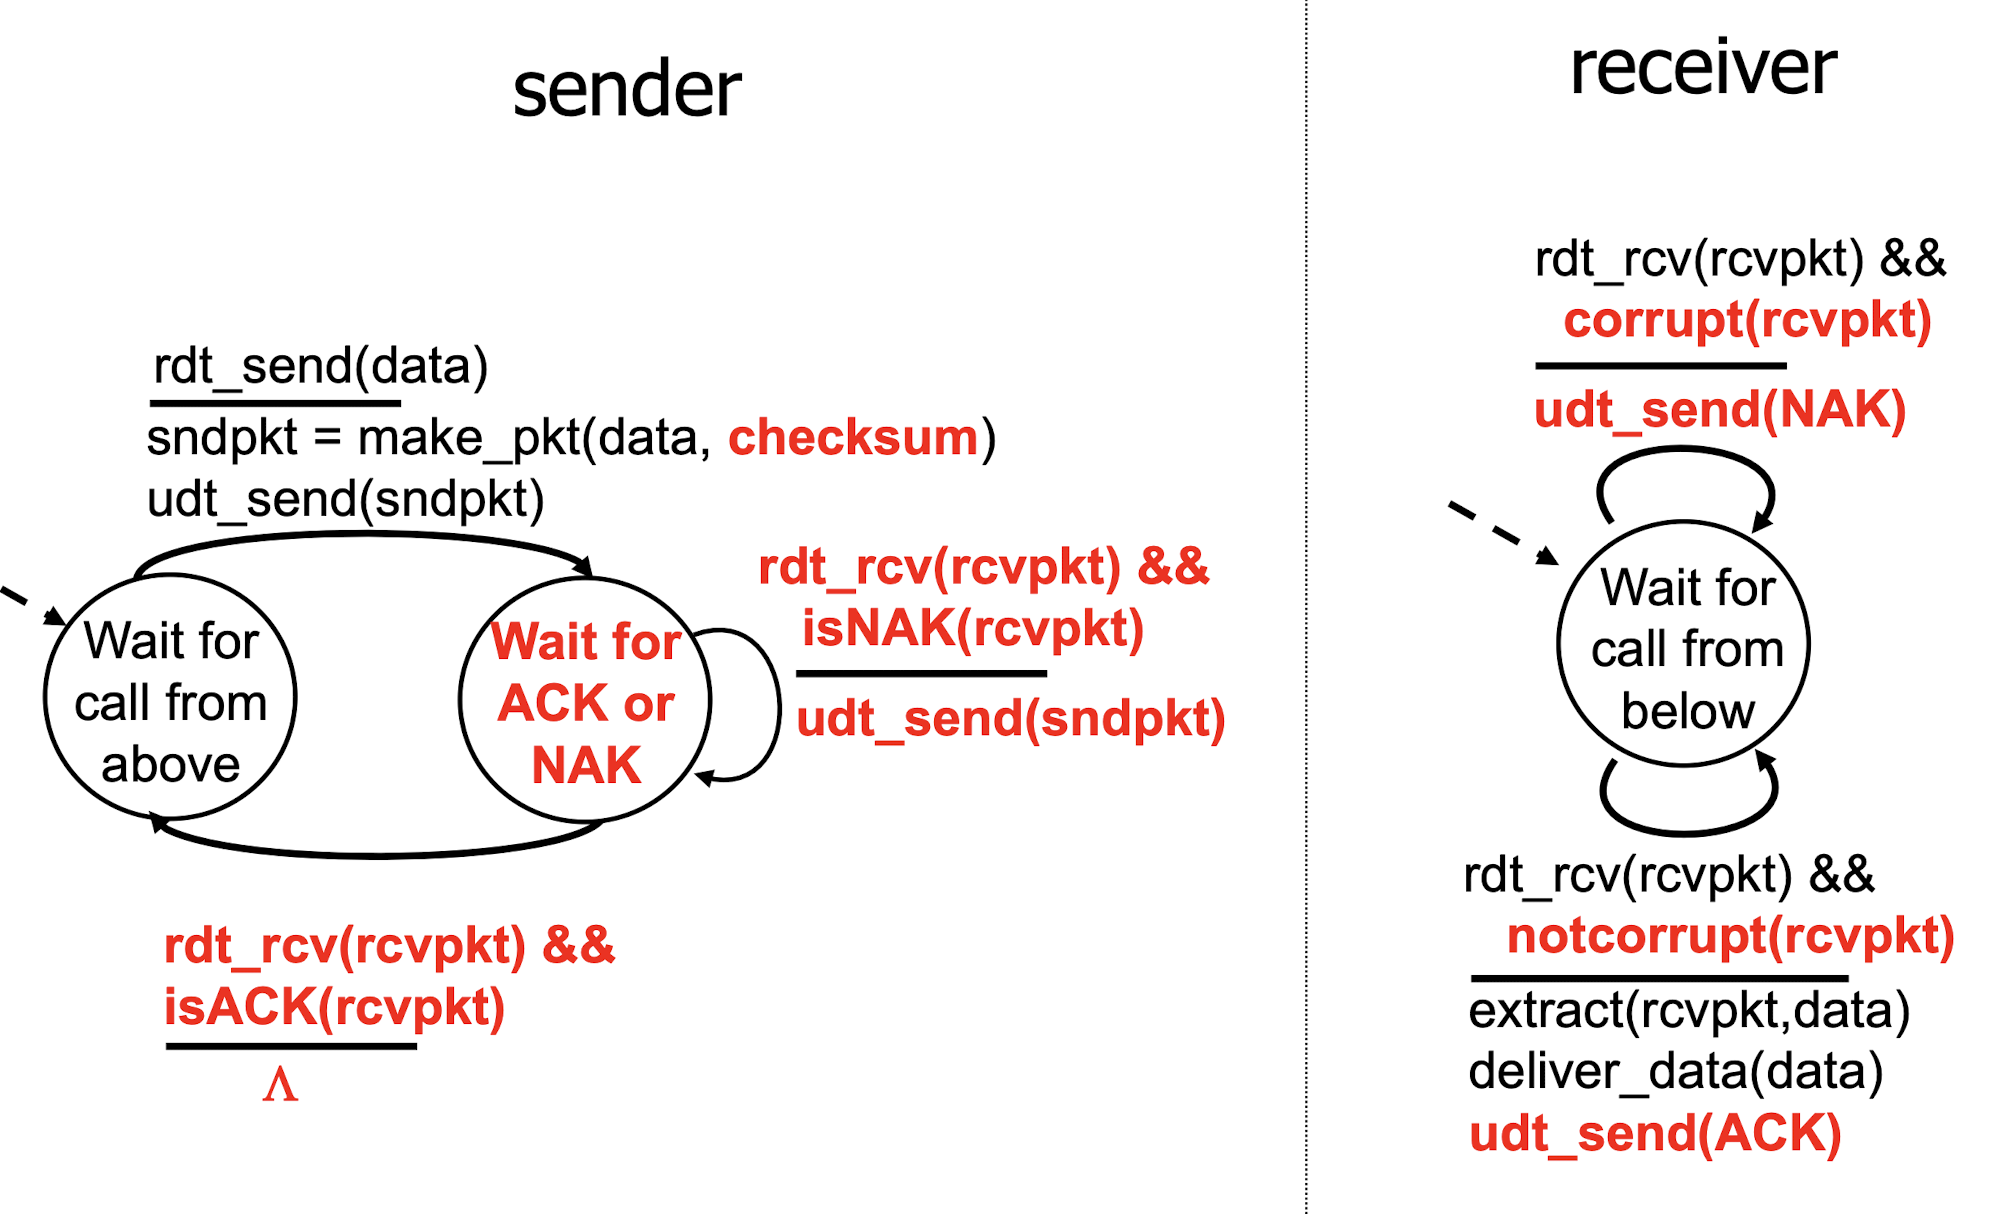
\includegraphics[scale=0.2]{rdt-2.0-fsm}

\subsubsection{rdt 2.1}

\begin{itemize}
    \item New problem: ACK/NAK may be corrupted
    \item Solution: Sender retransmits packet after receiving corrupted ACK/NAK
    \item New problem: Duplicate packets during retransmission
    \item Solution: Sender adds \textbf{sequence number} to each packet and receiver discards duplicate packet (Only 0 and 1 needed)
\end{itemize}

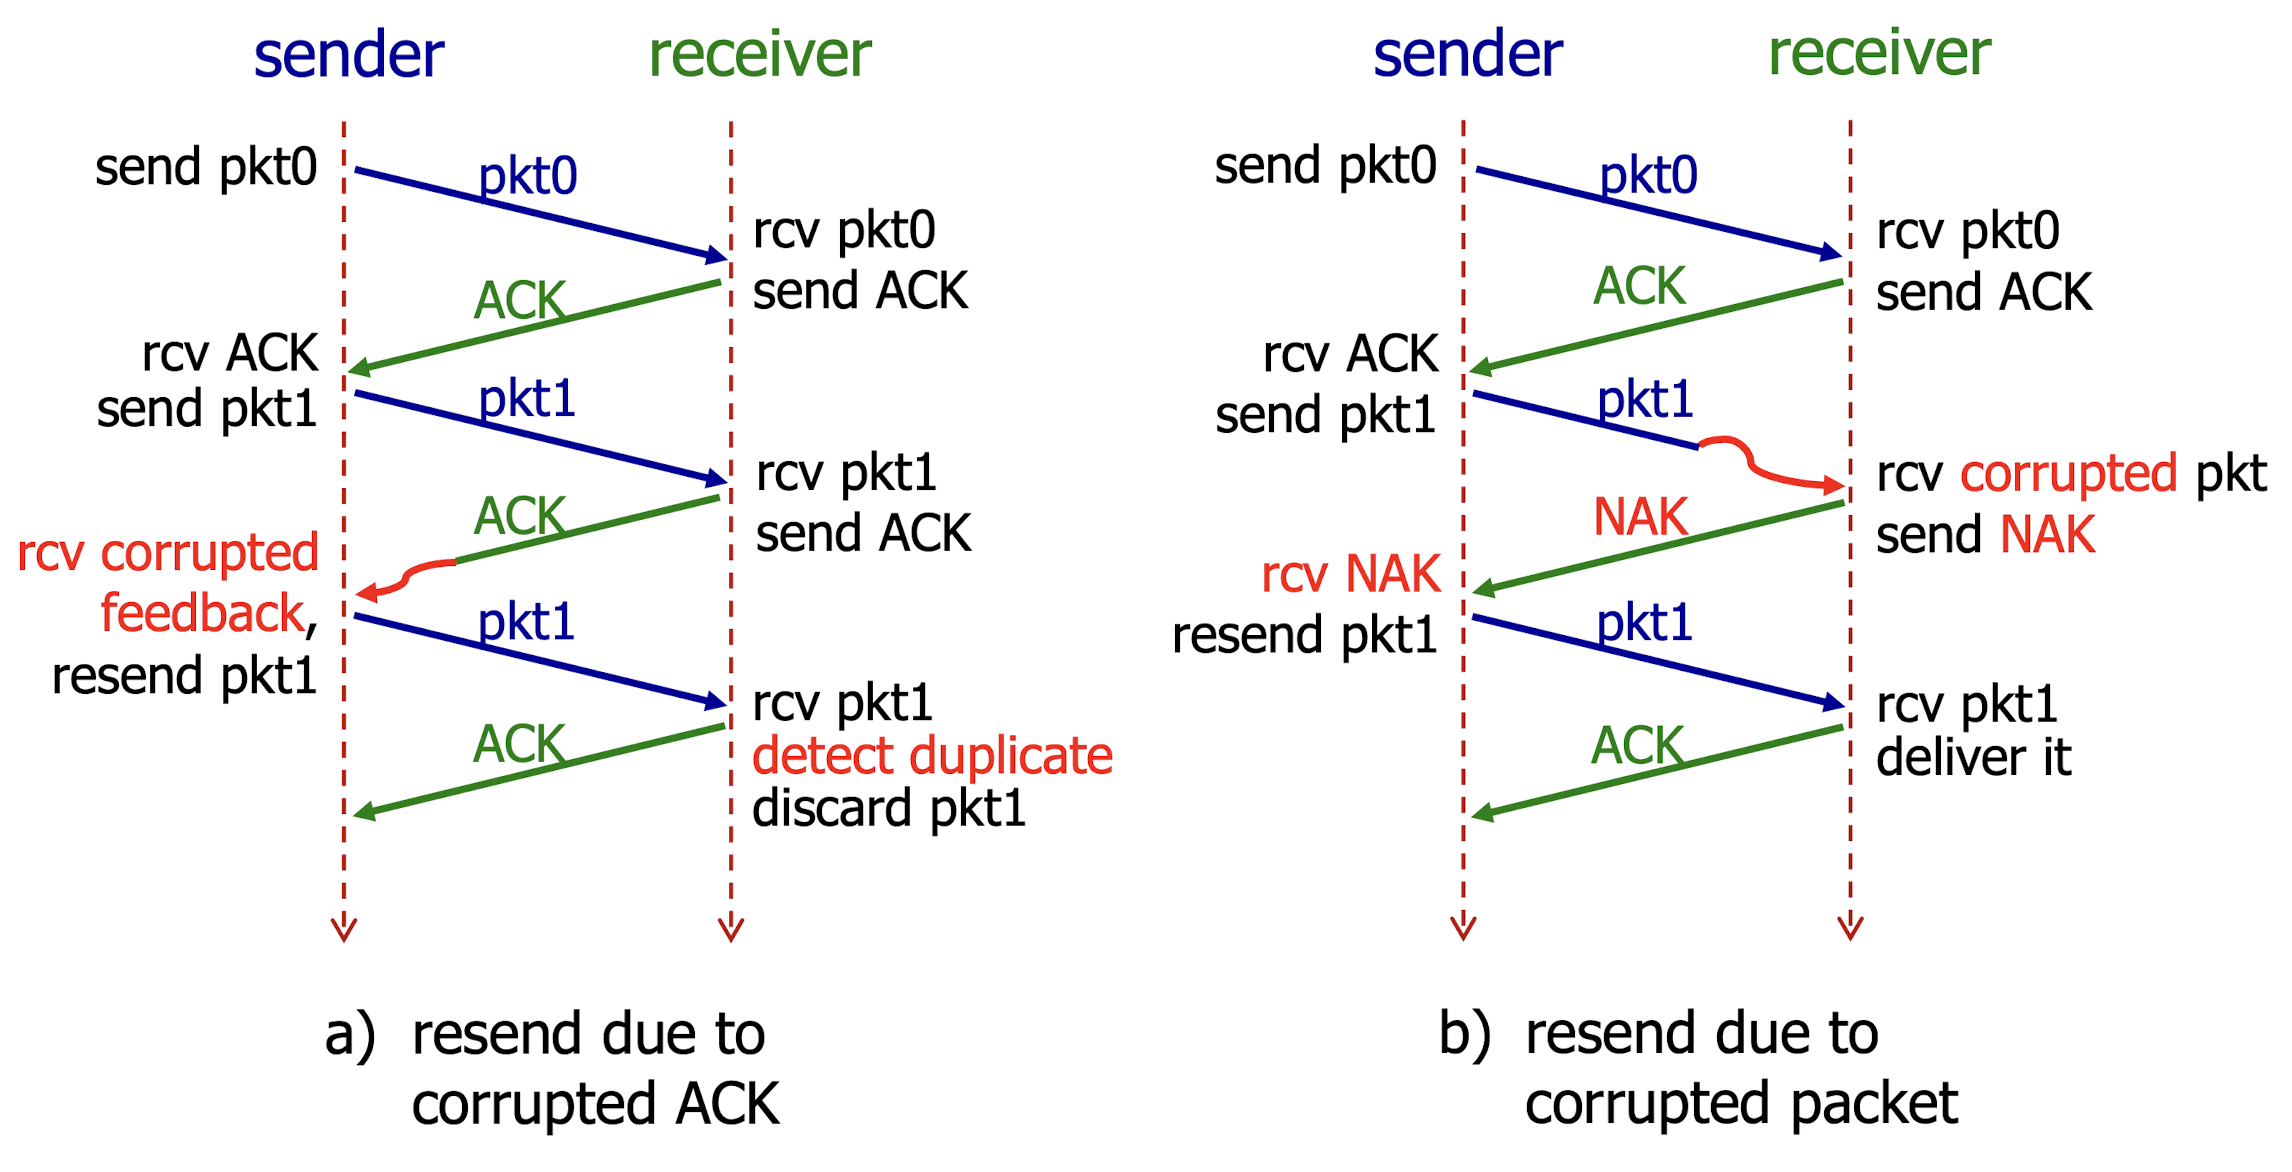
\includegraphics[scale=0.2]{rdt-2.1}

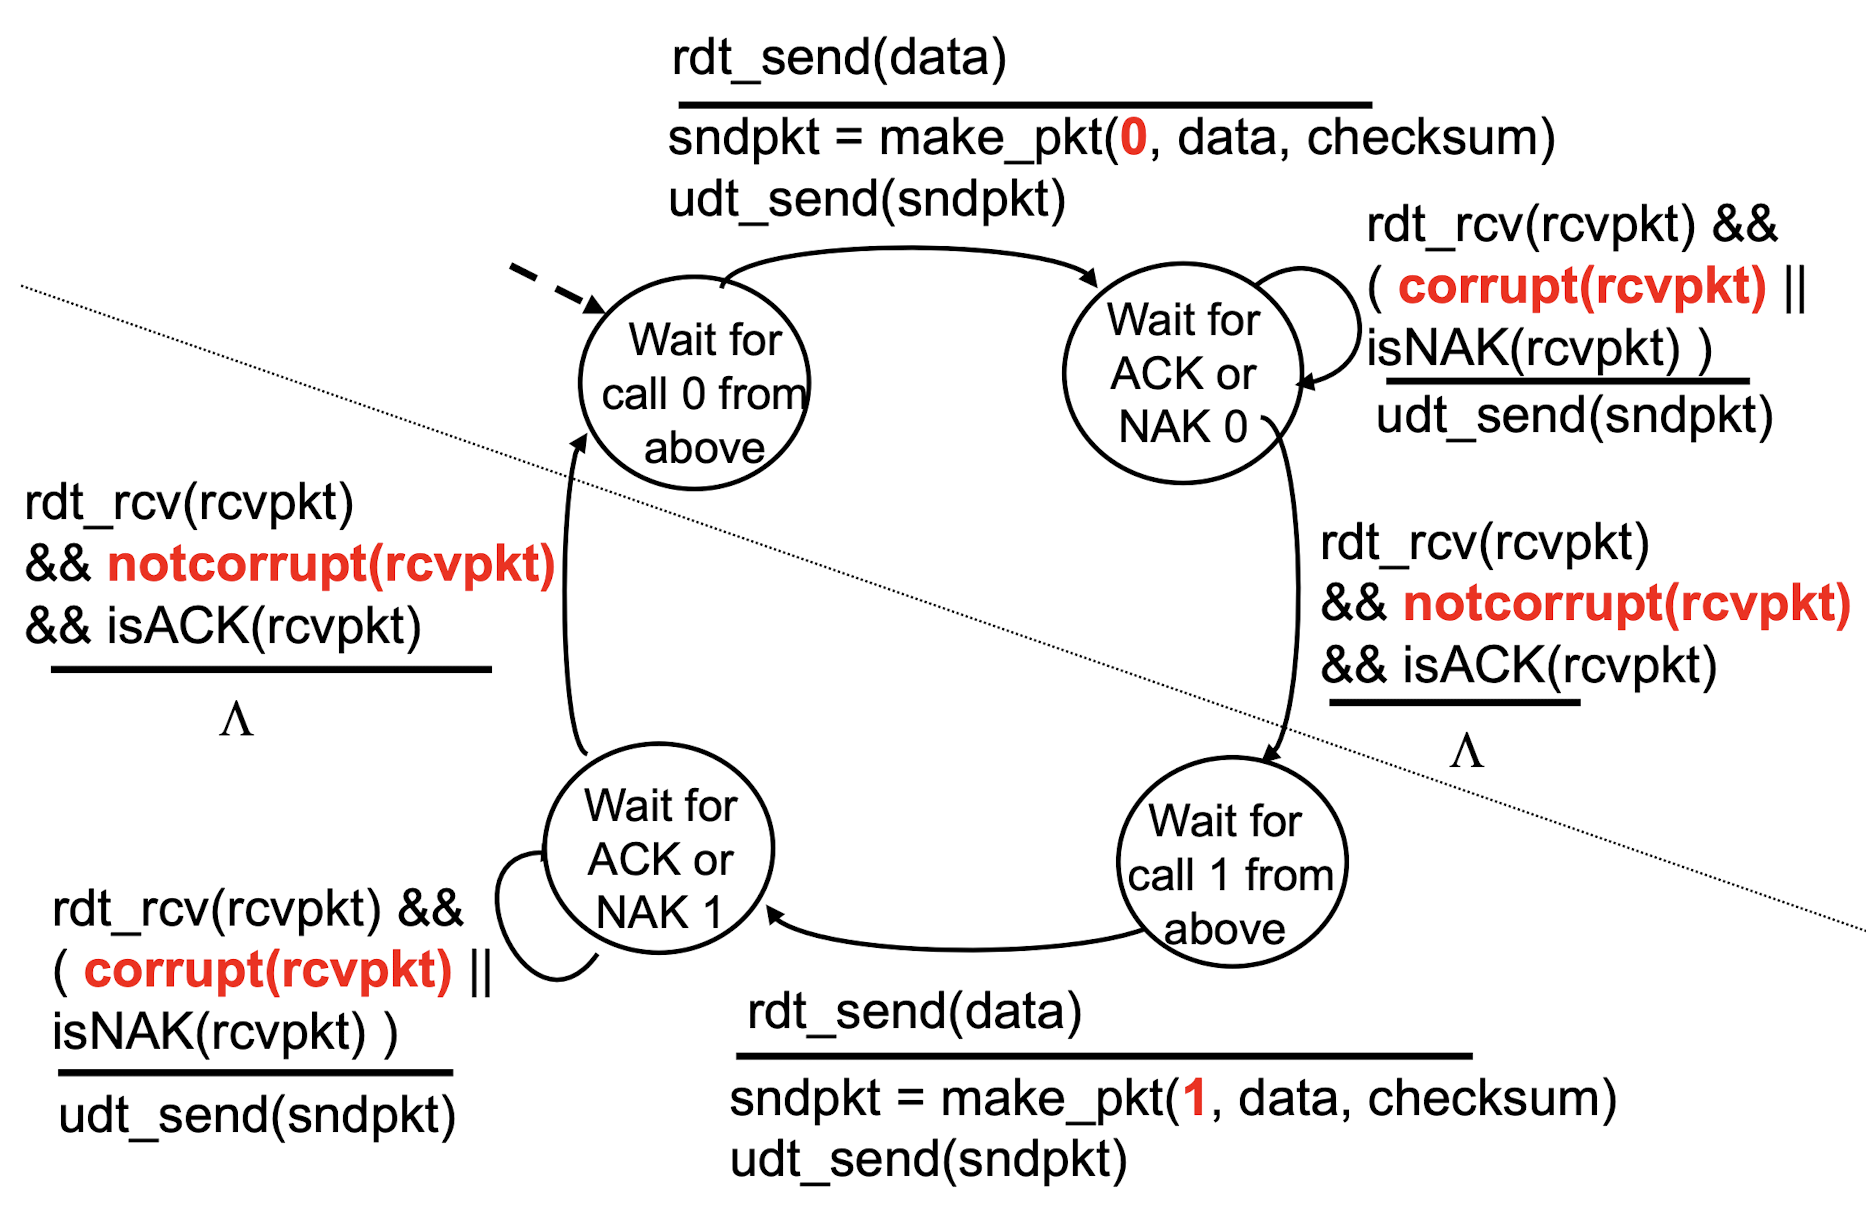
\includegraphics[scale=0.2]{rdt-2.1-sender-fsm}

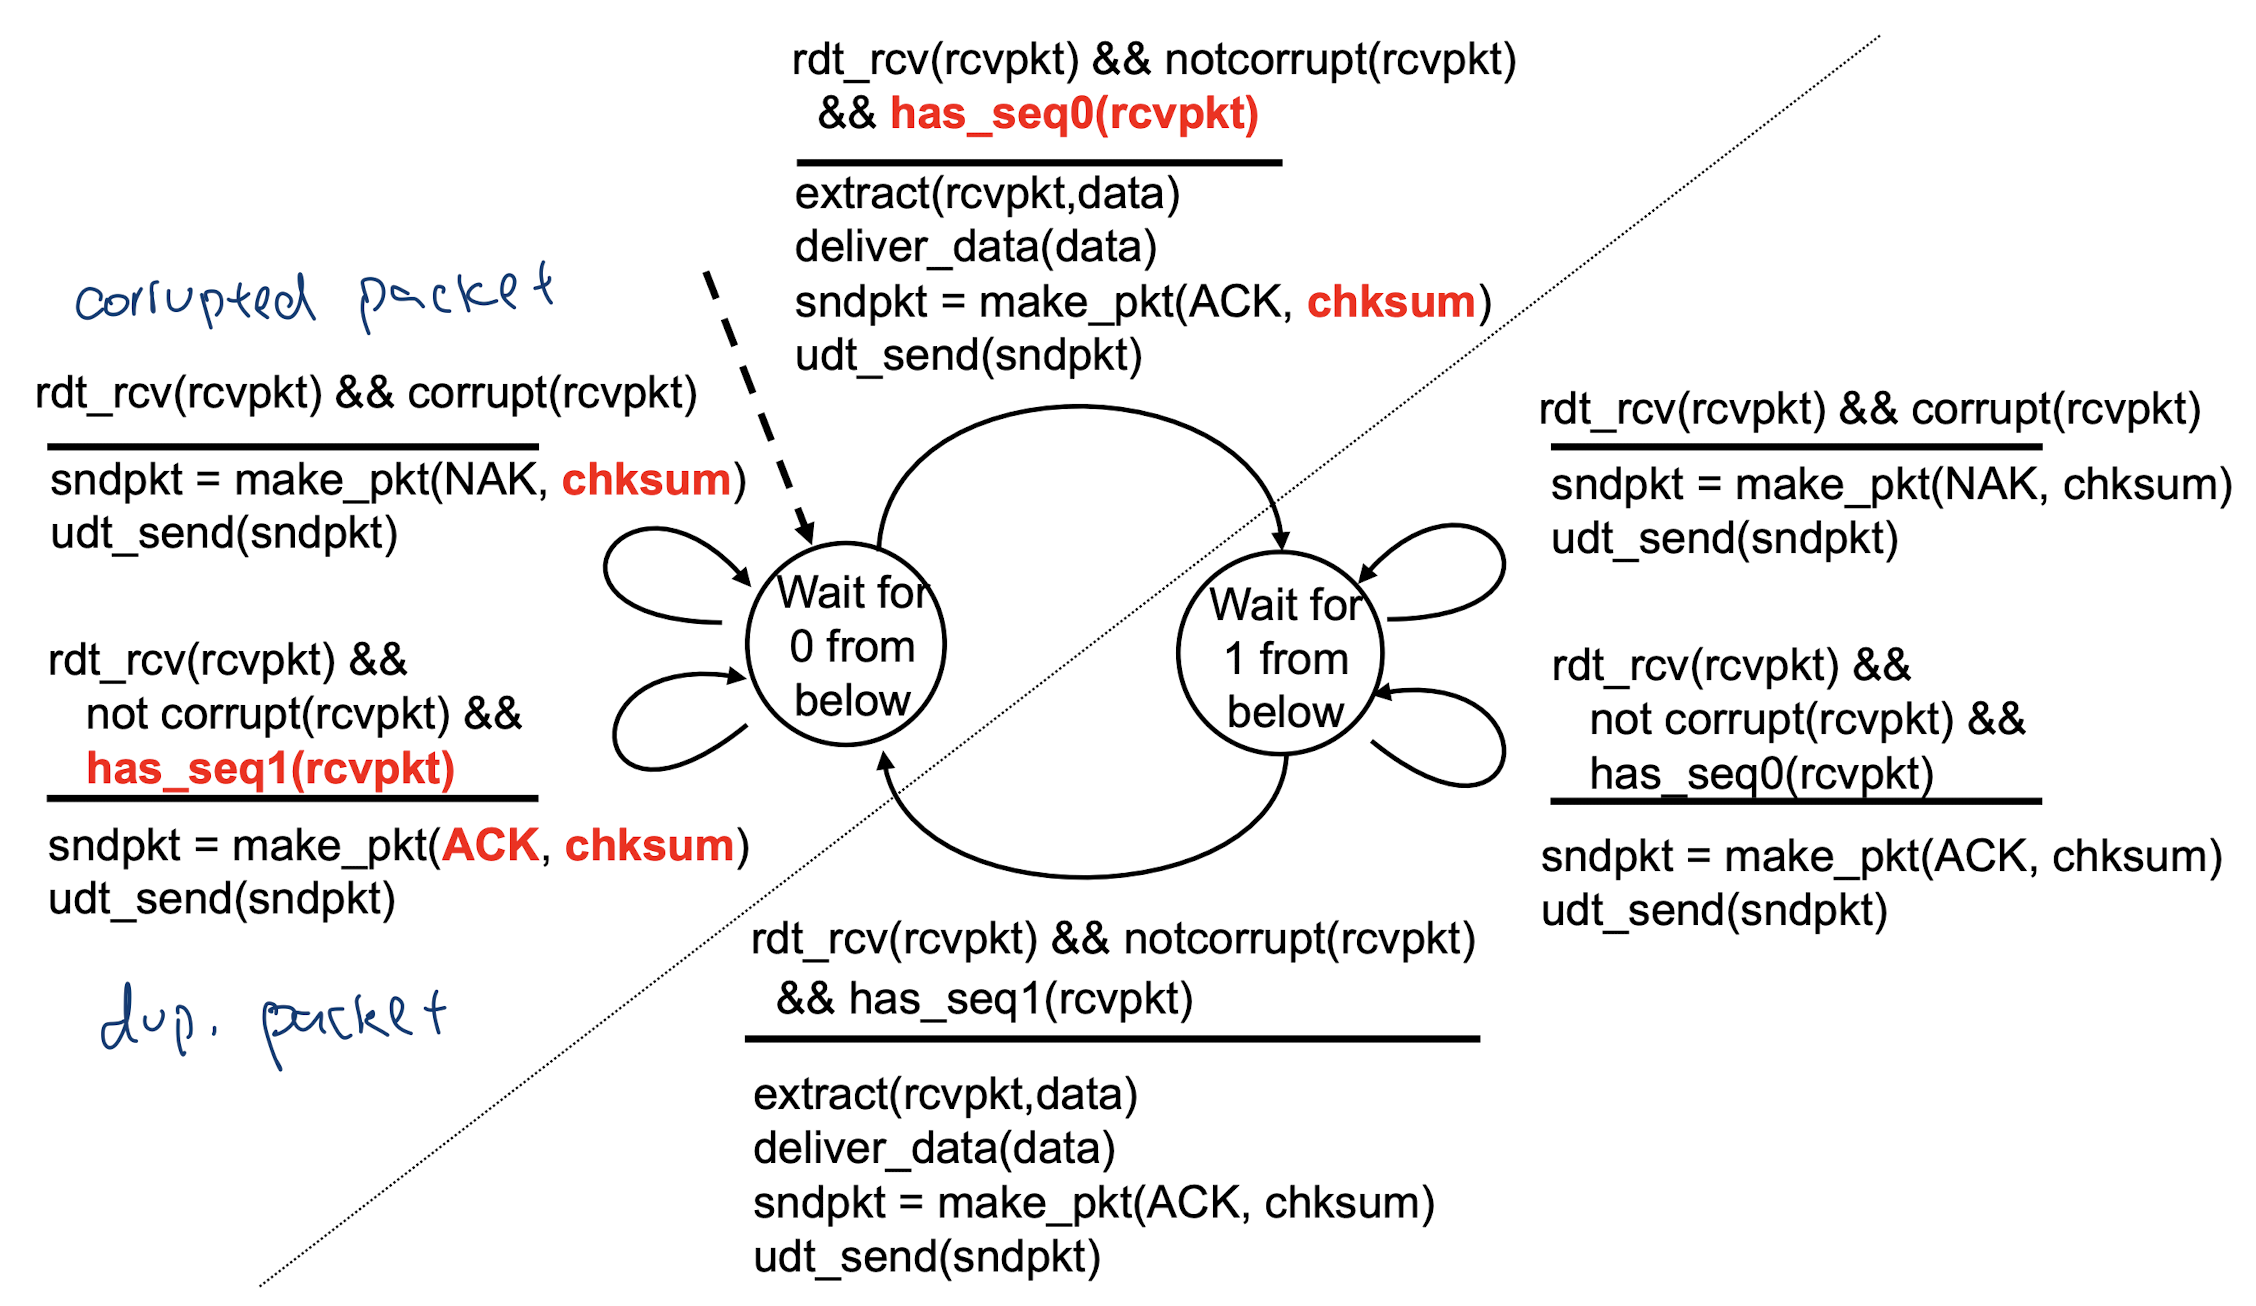
\includegraphics[scale=0.2]{rdt-2.1-receiver-fsm}

\subsubsection{rdt 2.2}

\begin{itemize}
    \item No NAK, only ACKs
    \item Receiver sends ACK for last packet received. \textbf{ACK must include seq number of packet}.
    \item Receiver send duplicate ACK to retransmit current packet
\end{itemize}

\subsubsection{rdt 3.0}

\begin{itemize}
    \item New problem: Lost packets
    \item Solution: Sender waits for some time for ACK and retransmits packet
    \begin{itemize}
        \item What if duplicate packet? Sequence number handles this.
        \item What if duplicate ACK? Do nothing.
    \end{itemize}
\end{itemize}

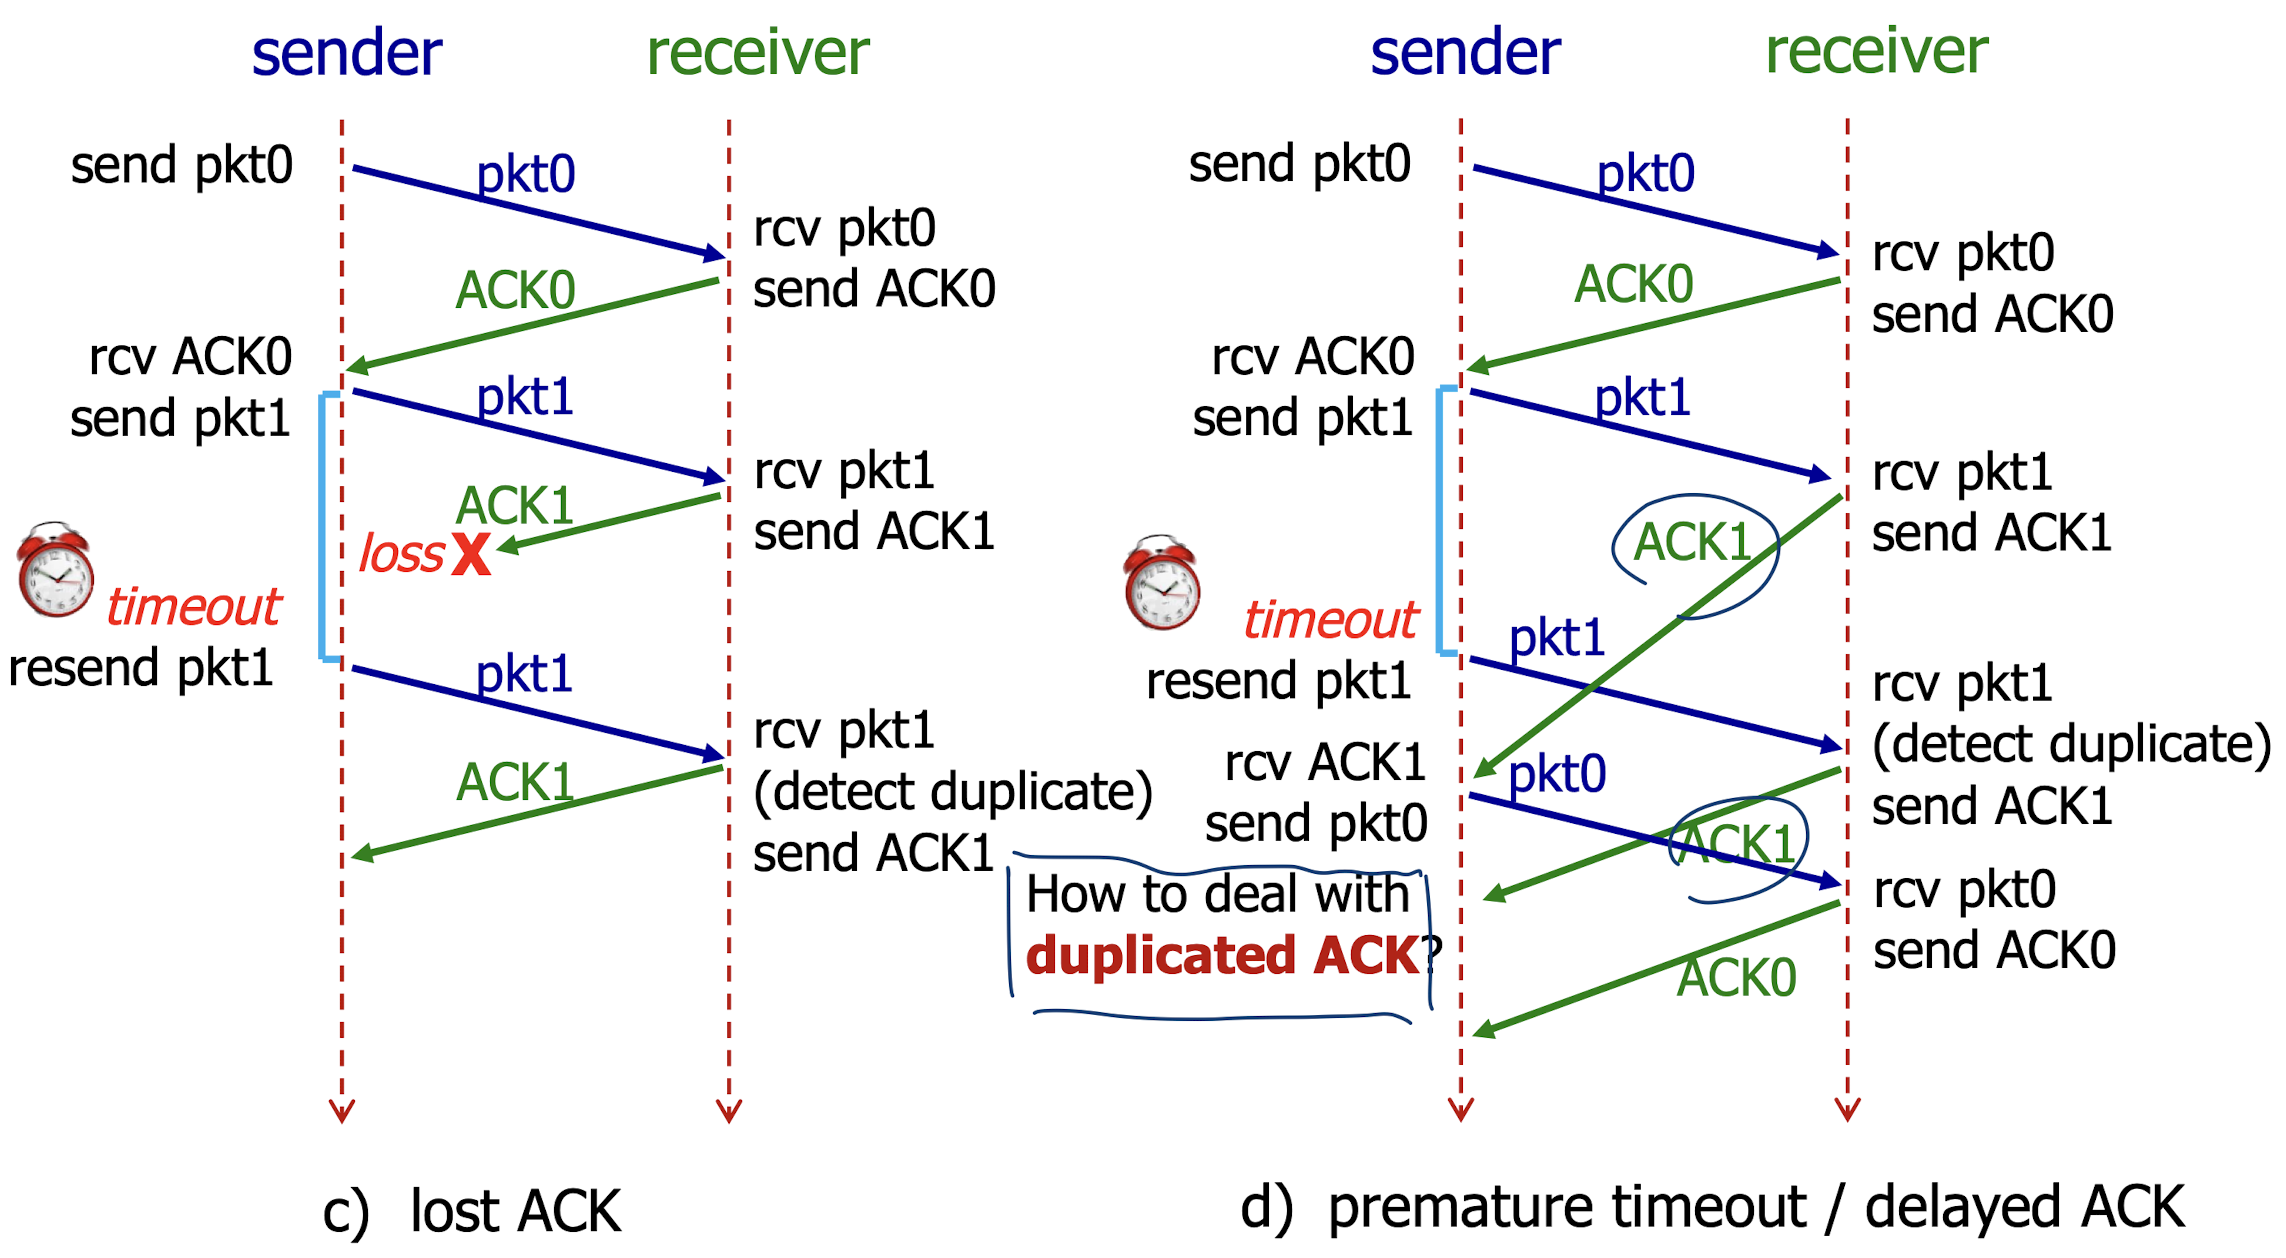
\includegraphics[scale=0.2]{rdt-3.0-1}

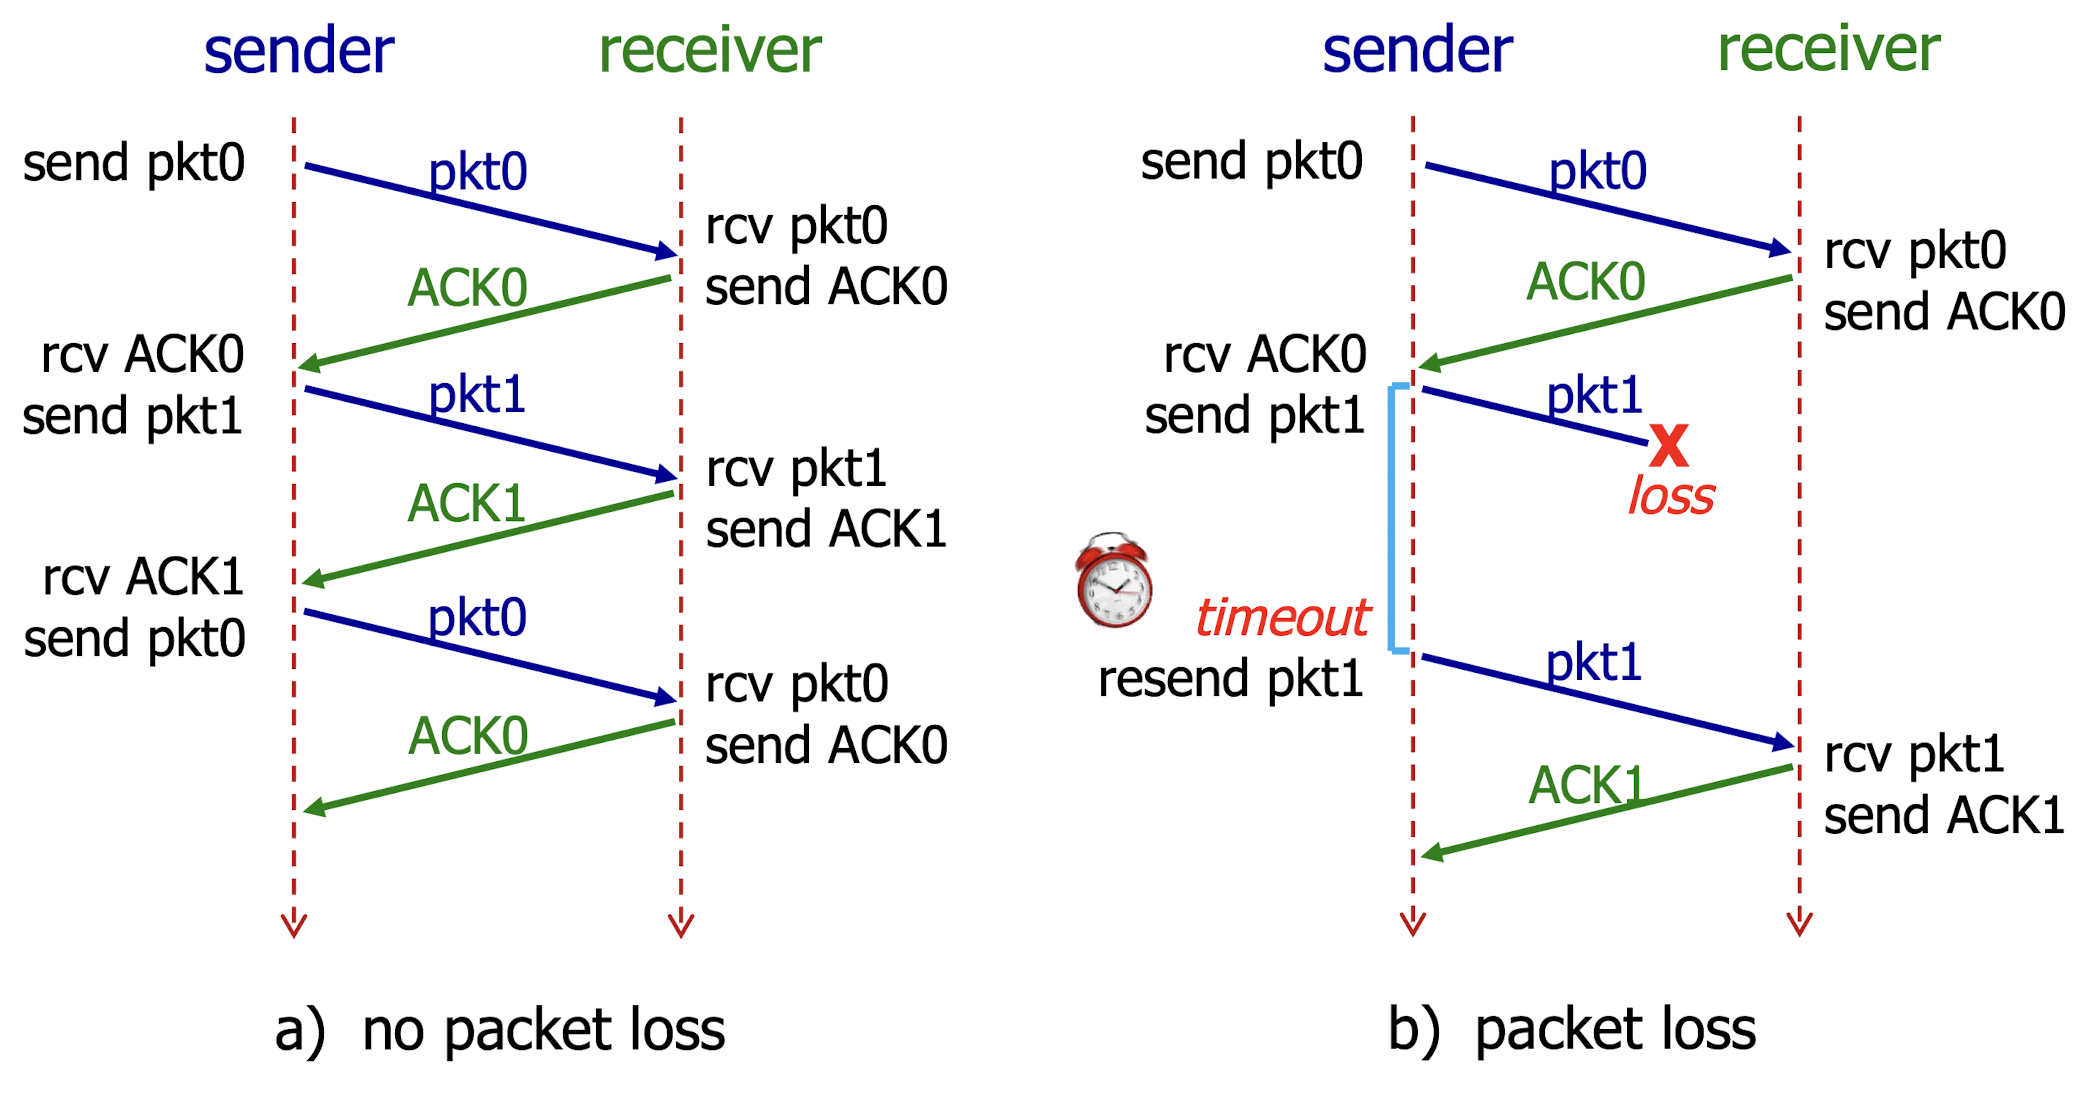
\includegraphics[scale=0.2]{rdt-3.0-2}

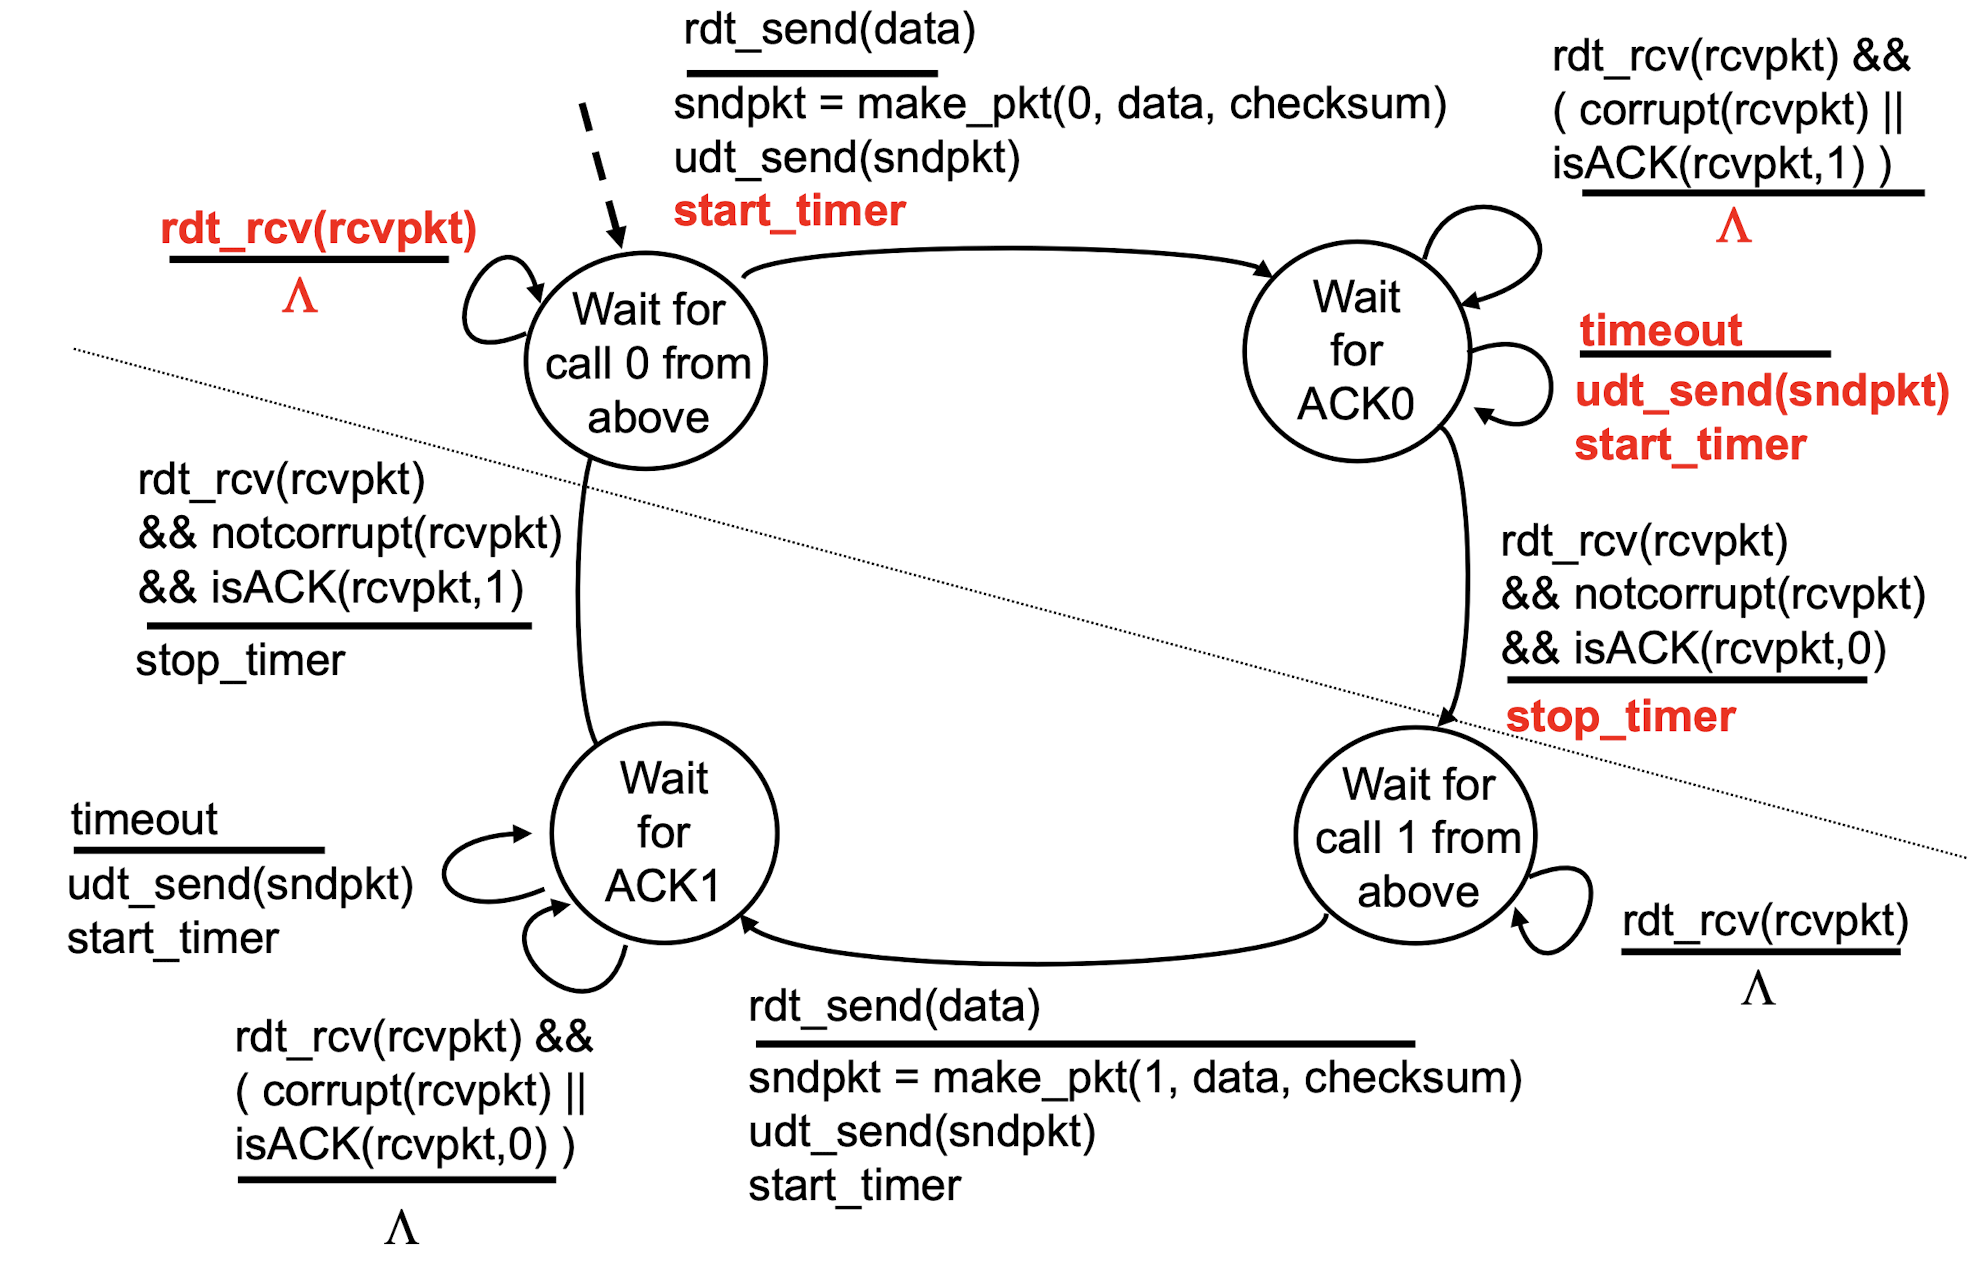
\includegraphics[scale=0.2]{rdt-3.0-fsm}

\subsubsection{Performance of rdt 3.0}

\begin{itemize}
    \item \keyword{Stop-and-wait protocol}{Sender sends 1 packet at a time, then waits for receiver response}
    \item Performance is bad. Stop-and-wait protocol limits use of resources
    \item \keyword{Utilization}{Fraction of time sender is busy sending}
    \begin{itemize}
        \item Given: 1 Gbps link, 15 ms prop. delay, 8000 bit packet
        \item $D_{trans} = \frac{L}{R} = \frac{8000 bits}{10^9 bits / sec} = 8 microsecs$
        \item $U_{sender} = \frac{D_{trans}}{RTT + D_{trans}} = \frac{0.008}{30.008} = 0.027\%$
        \item Pipelined Utilisation = U * window\_size
    \end{itemize}
\end{itemize}

\subsubsection{Pipelined Protocols}

\begin{itemize}
    \item \keyword{Pipelining}{Sender allows multiple not-yet-ACKed packets}
    \begin{itemize}
        \item Need more sequence numbers
        \item Buffering at sender and receiver
    \end{itemize}
\end{itemize}
Pipeline vs Parallel (HTTP)
\begin{itemize}
	\item Parallel connections need to retrieve HTML webpage first before retrieving data elements
	\item Pipeline can retrieve HTML and data elements all at once

\end{itemize}

\subsection{Go-Back-N}

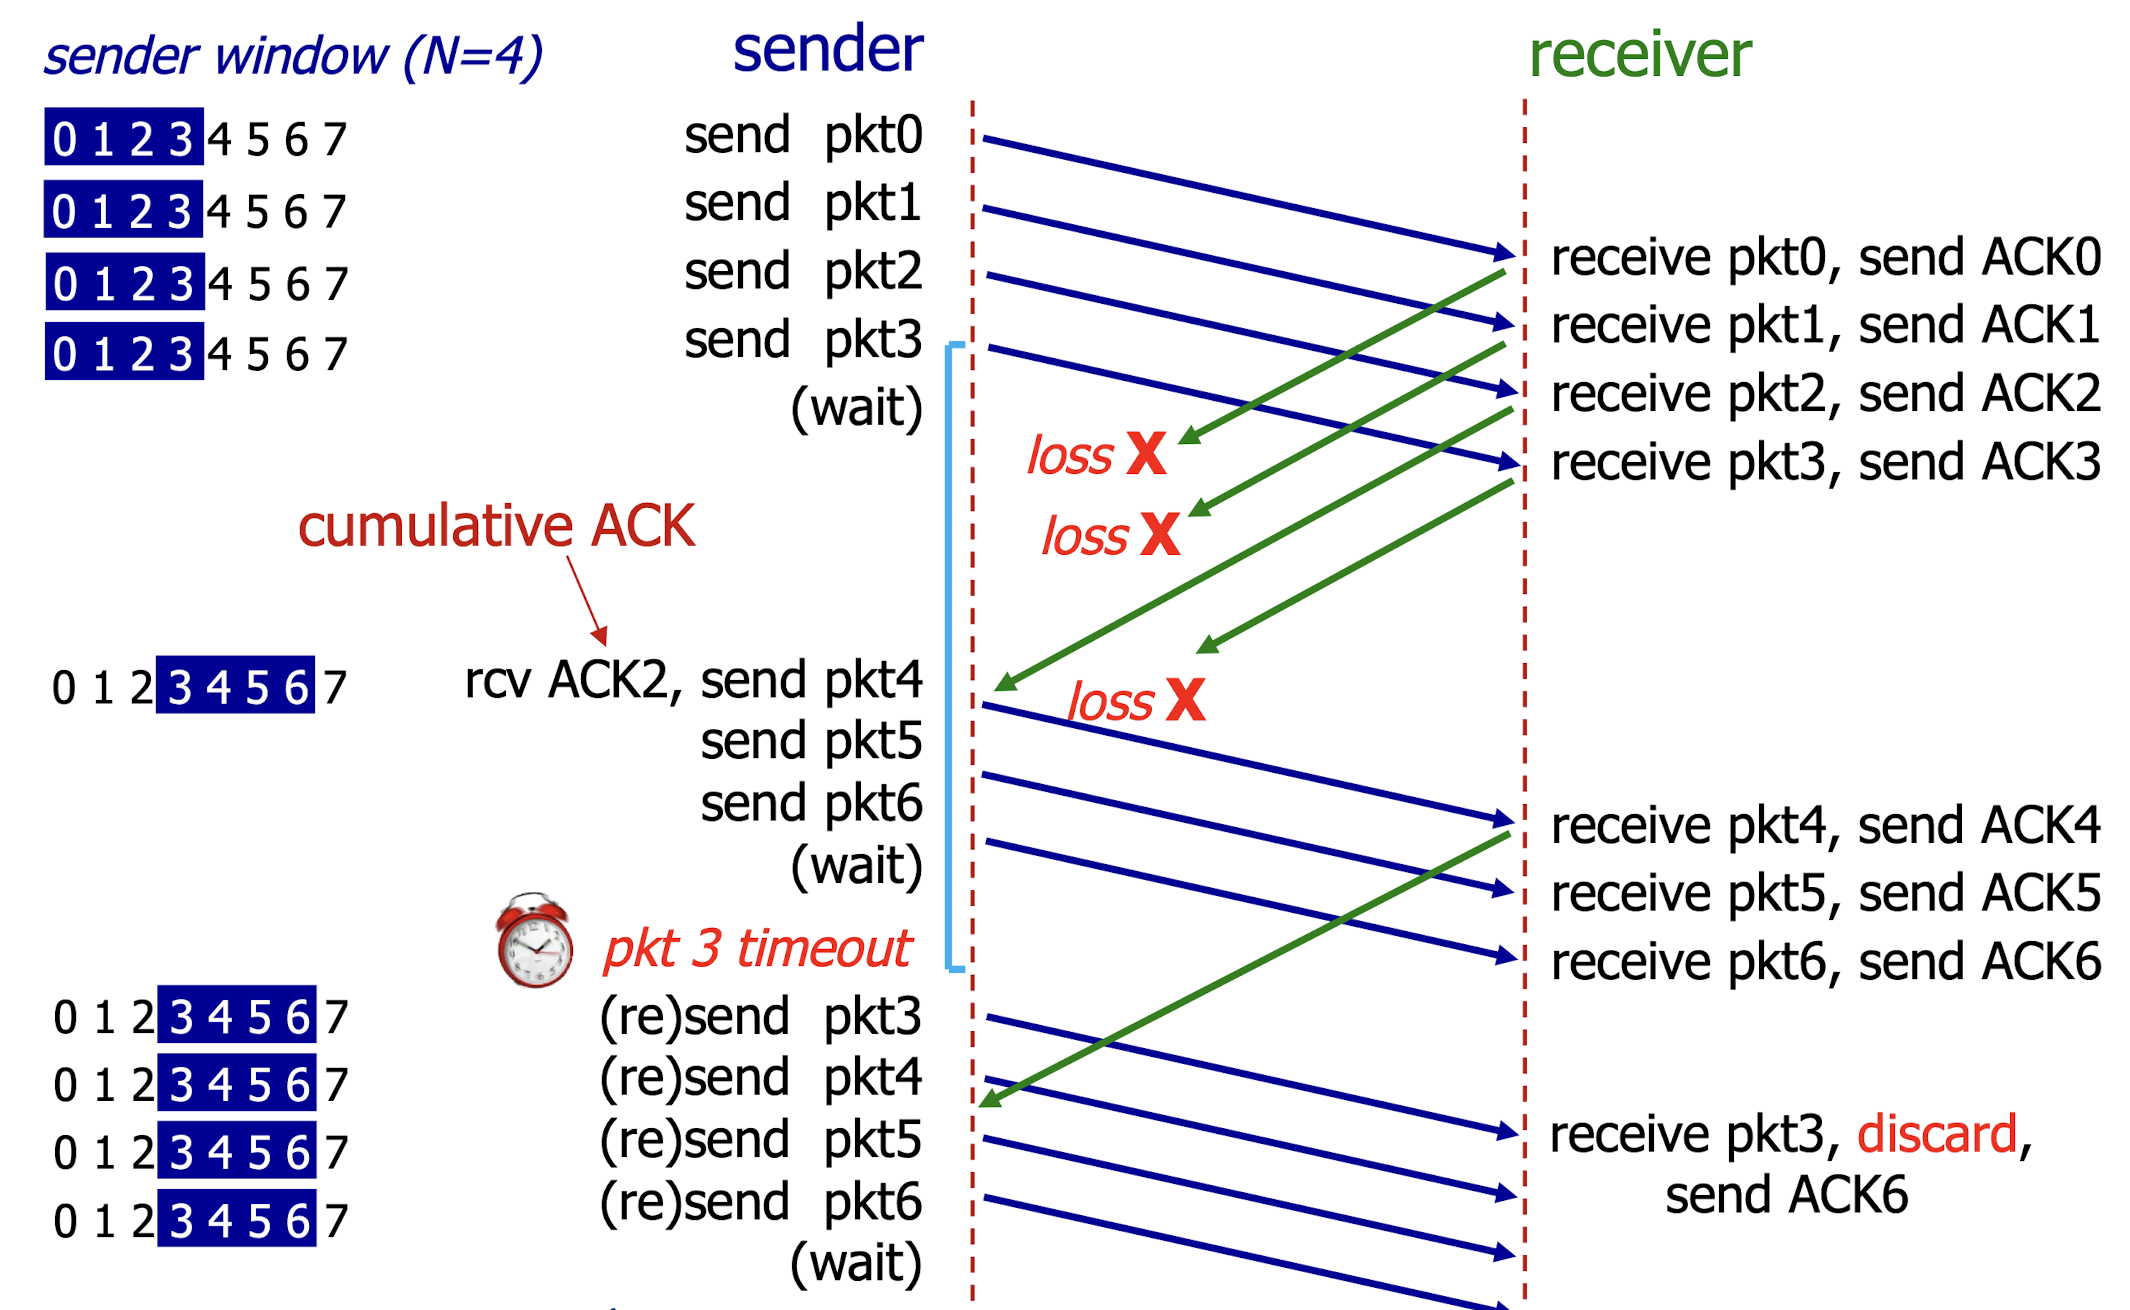
\includegraphics[scale=0.17]{go-back-n}

\begin{itemize}
    \item Intuition: Sliding window
    \item Sender:
    \begin{itemize}
        \item Timer for oldest in-flight packet
        \item If timeout($n$), retransmit packet $n$ and other pkts in window
    \end{itemize}
    \item Receiver:
    \begin{itemize}
        \item \keyword{Cumulative ACK}{ACK for correct pkt with highest in-order sequence}
        \item Only ACK packets that arrive \textbf{in-order}
        \item Discard \textbf{out-of-order} packets
    \end{itemize}
    \item Not efficient, since future packets discarded if out-of-order
\end{itemize}

\subsection{Selective Repeat}

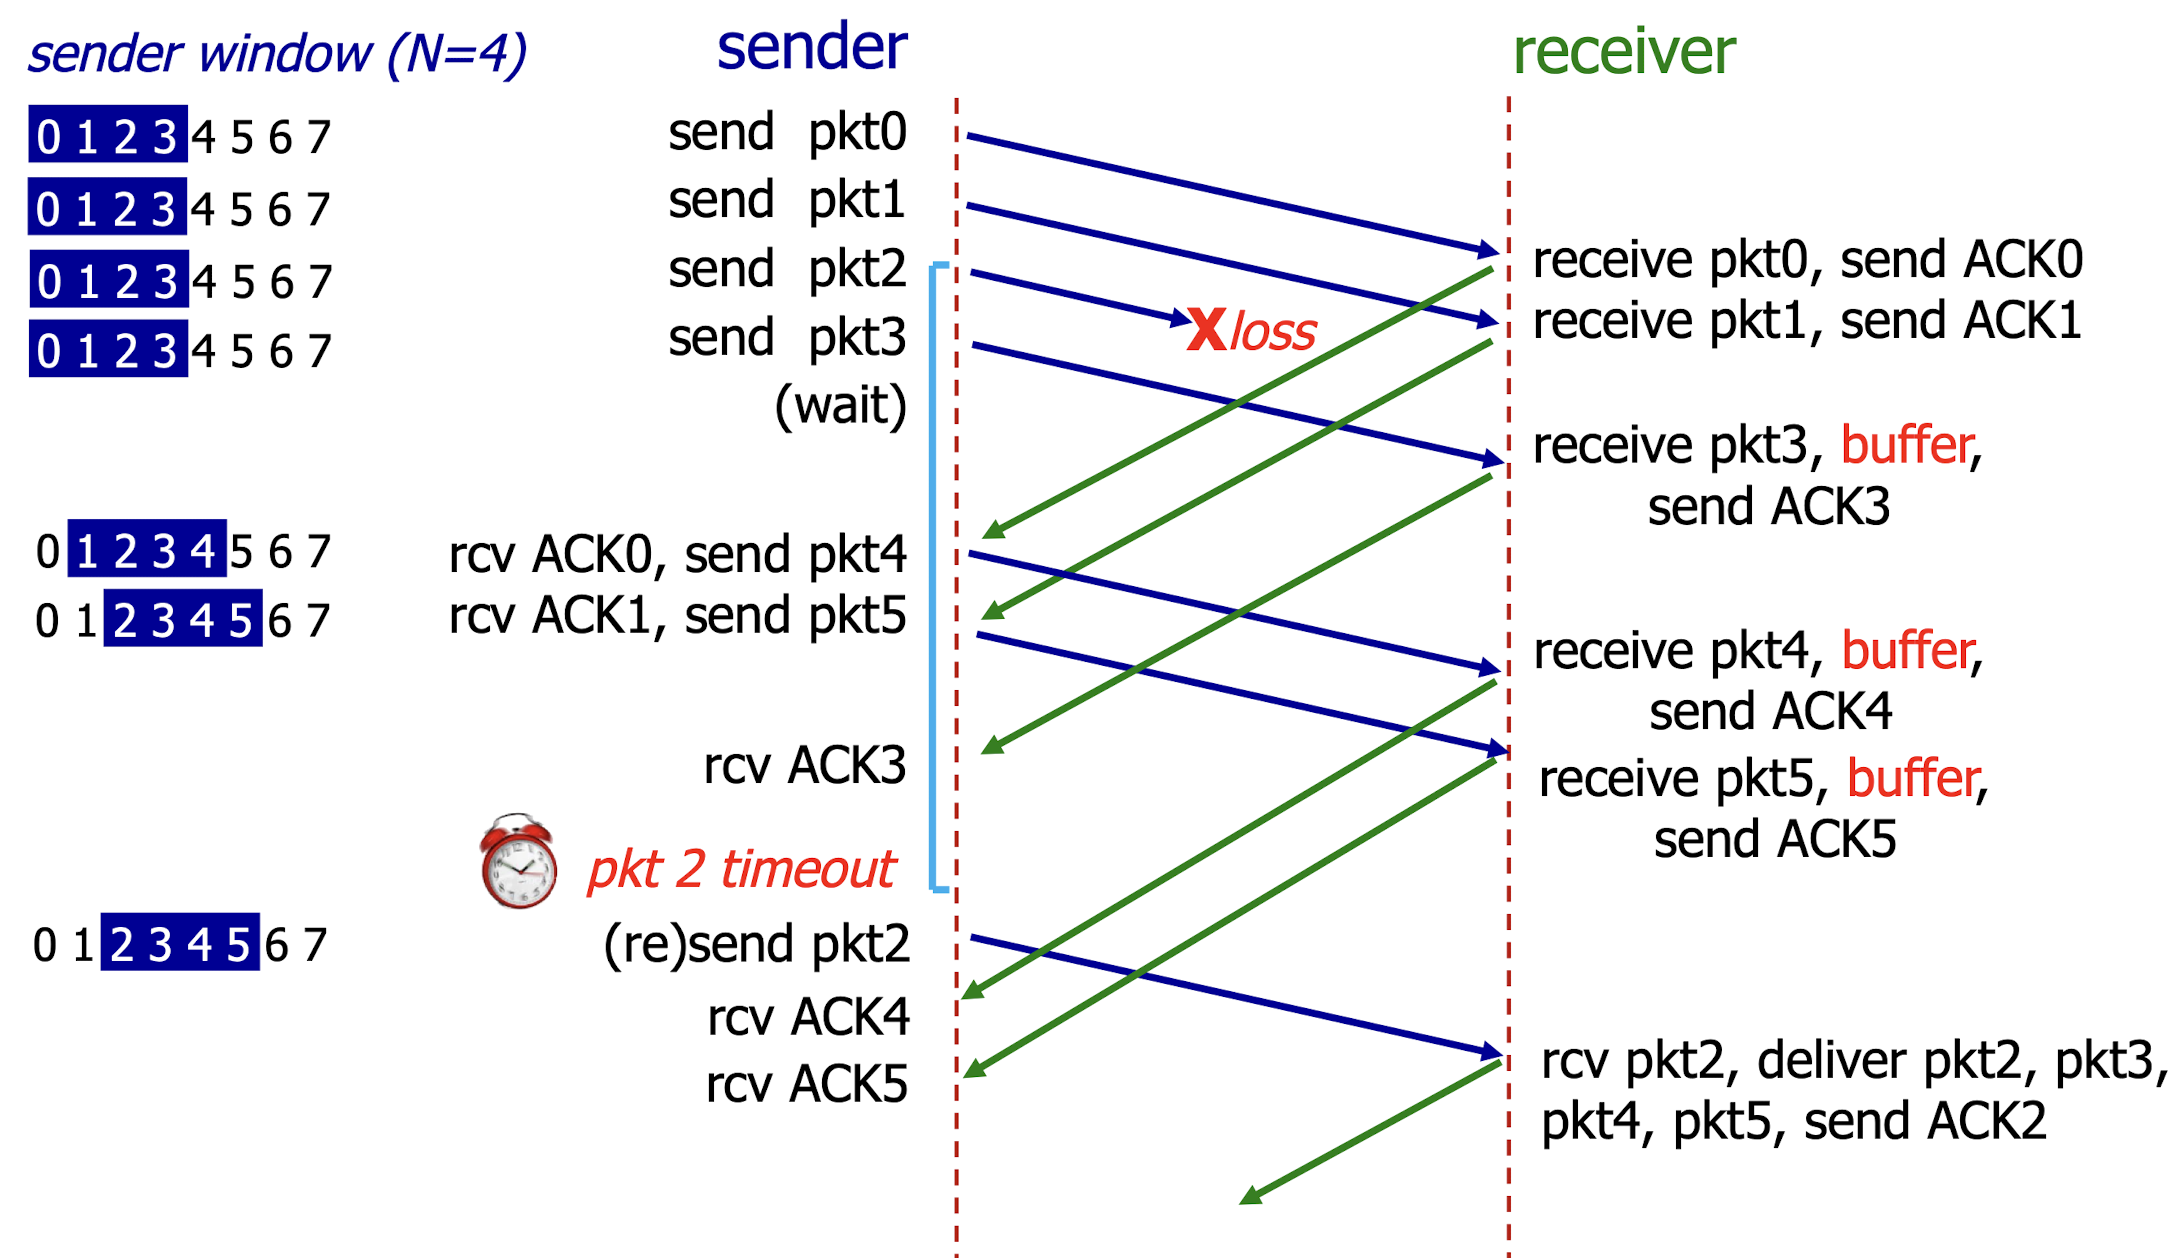
\includegraphics[scale=0.2]{selective-repeat}

\begin{itemize}
    \item Receiver individually ACKs correct pkts (Not accumulative) and sender maintains timer for each unACKed pkt
    \item Sender:
    \begin{itemize}
        \item If timeout($n$), retransmit packet $n$ only
        \item If ACK($n$) and $n$ is smallest unACKed pkt, slide window
    \end{itemize}
    \item Receiver:
    \begin{itemize}
        \item Once receive pkt $n$ in window, send ACK($n$). If out-of-order, buffer. If in-order, deliver and slide window
        \item Once receive pkt $n$ outside of window, still send ACK($n$)
        \item ACK m == packet m received but has no implication on receipt of other packets
    \end{itemize}
\end{itemize}


% -----------------------------------------------------------------------
\section{05. TCP}
\subsection{TCP Features}
\begin{itemize}
	\item \keyword{Point-to-point}{1 sender and 1 receiver}
	\item \keyword{Connection-oriented}{Handshaking before exchange data}
	\item \keyword{Full duplex}{Bi-directional data flow in connection}
	\item Reliable, in order and pipelined
	\item Buffers on both hosts
	\item Limited by \textbf{Maximum Segment Size} $\approx$ 1460B
	\begin{itemize}
		\item Refers only to content length (no header)
		\item Limited by \keyword{MTU}{Maximum transmission unit, size of largest IP transaction}
	\end{itemize}
\end{itemize}
\subsection{Structure}
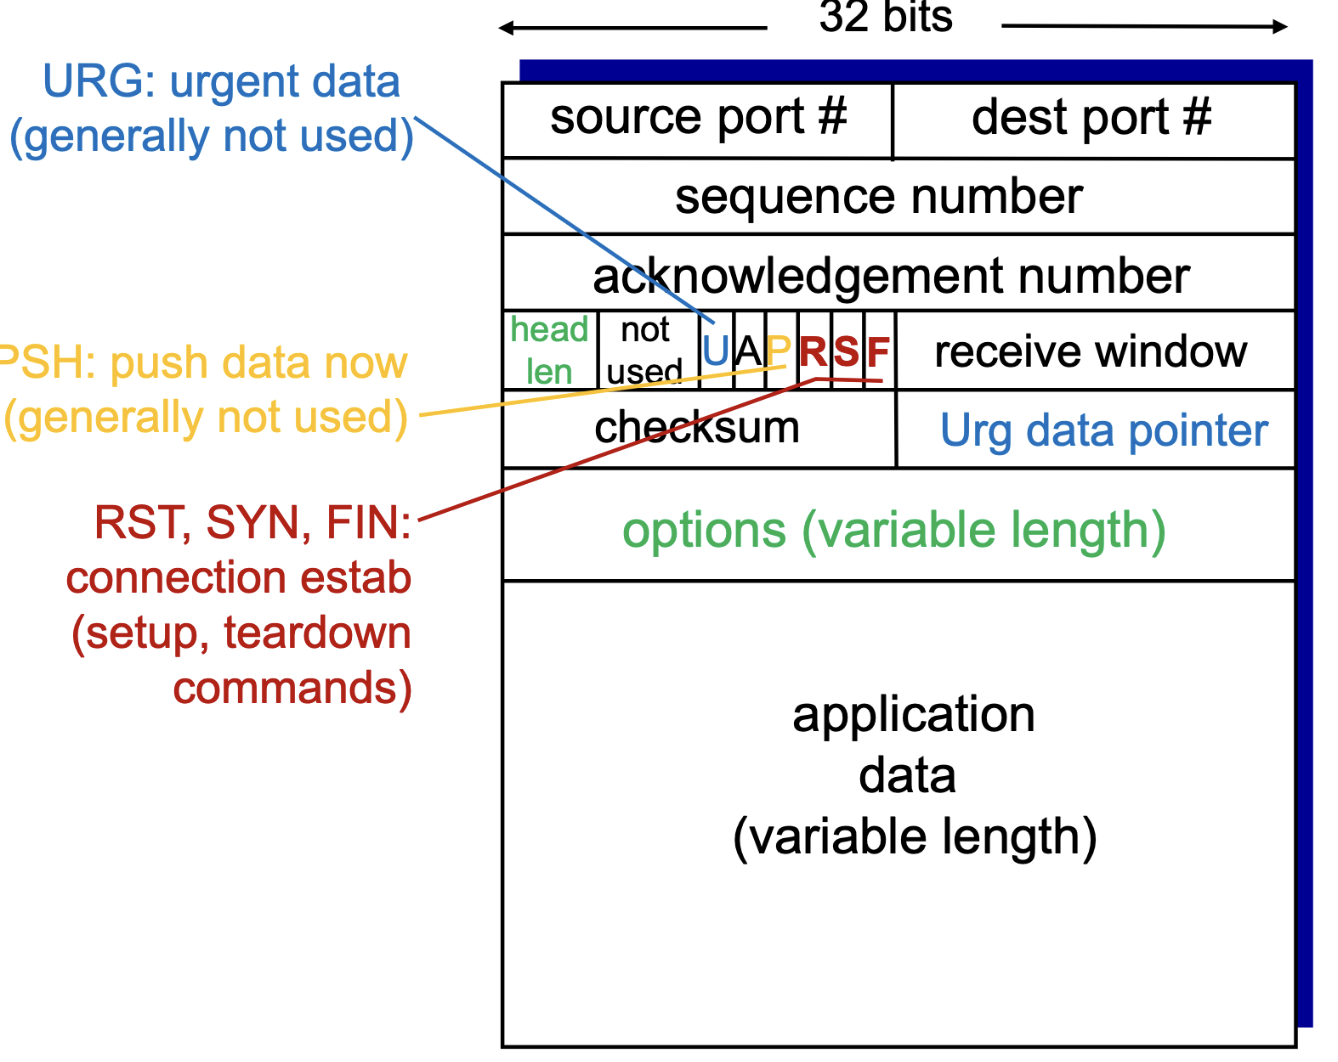
\includegraphics[scale=0.3]{tcp-structure}
\\Header is 20-60 bytes long
\begin{enumerate}
	\item Sequence \#
	\begin{itemize}
		\item Let receiver know if packet is retransmission or new data
		\item Value only measures the body length in bytes
		\item Initial number randomly generated btw $0-(2^{32}-1)$ (Why?)
		\begin{itemize}
			\item Security
			\item Prevent duplicate sequence numbers when link is used extensively
		\end{itemize}
		\item ACK \# = next byte expected by receiver (inital seq \# + data length in bytes)
		\item SYN \# = byte number of first byte(expected ACK (of sender) - data length)
	\end{itemize}
	\item ACK number
	\item \keyword{rwnd}{Receive window}
	\begin{itemize}
		\item Number of bytes the receiver is willing to accept
		\item \keyword{Flow control}{Prevent overflow of receiver's buffer}
	\end{itemize}
	\item Flags - Connection establish or priority
\end{enumerate}

\subsection{Establish TCP connection}
Creates n+1 sockets for n clients (additional 1 for listening)\\
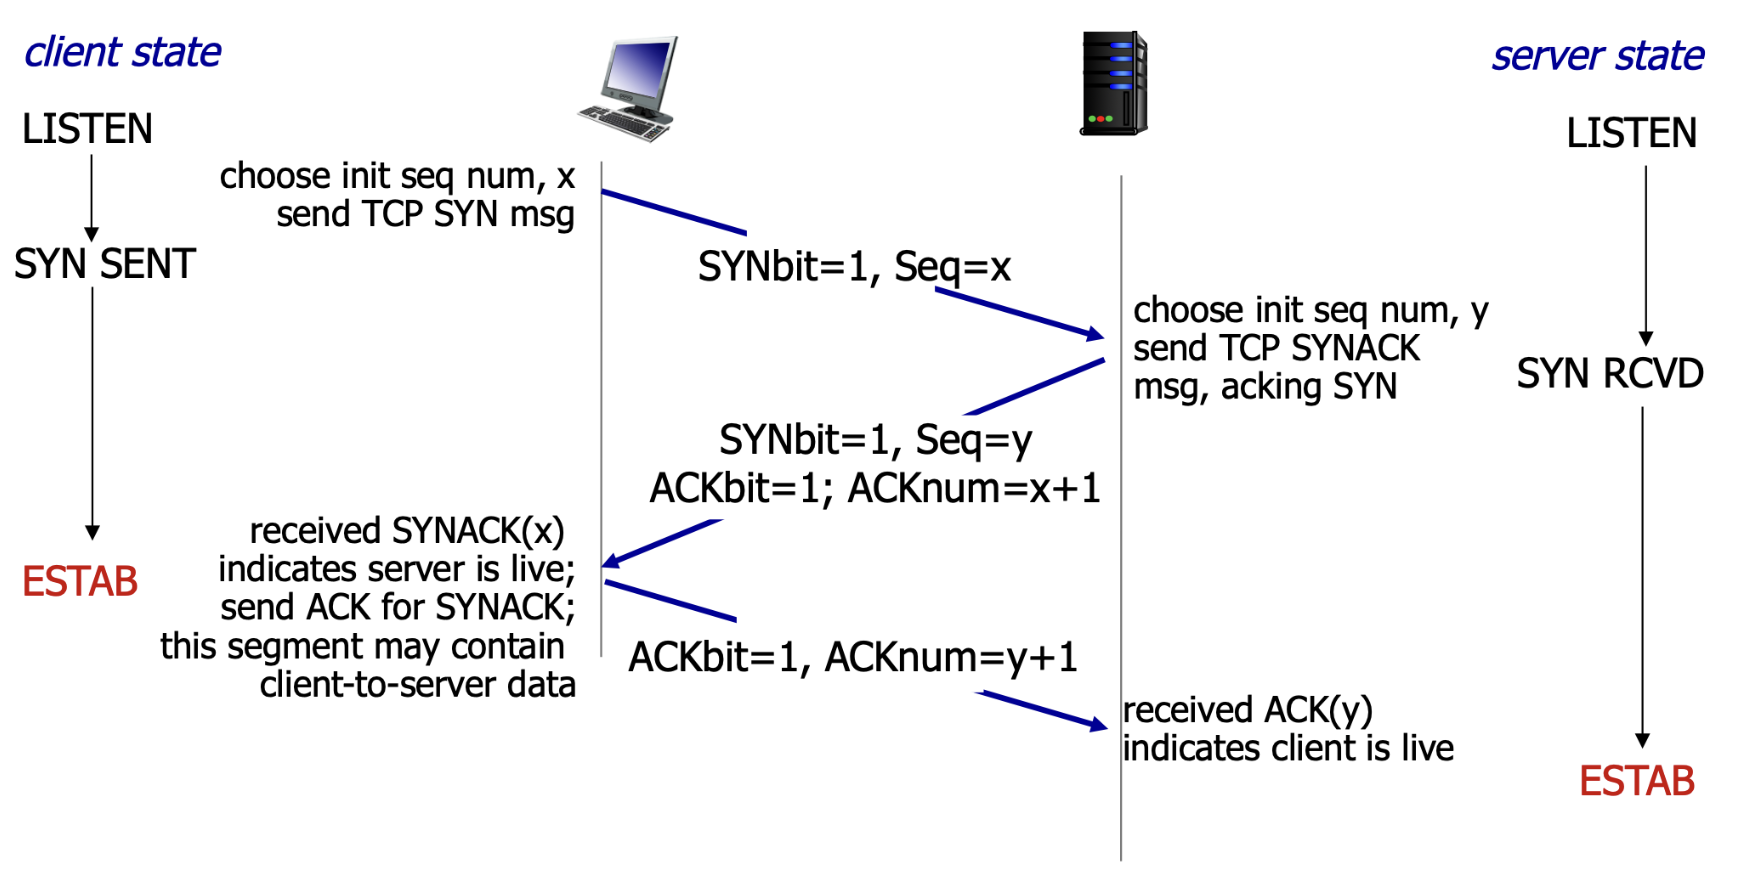
\includegraphics[scale=0.3]{tcp-estab}

\subsection{Close TCP connection}
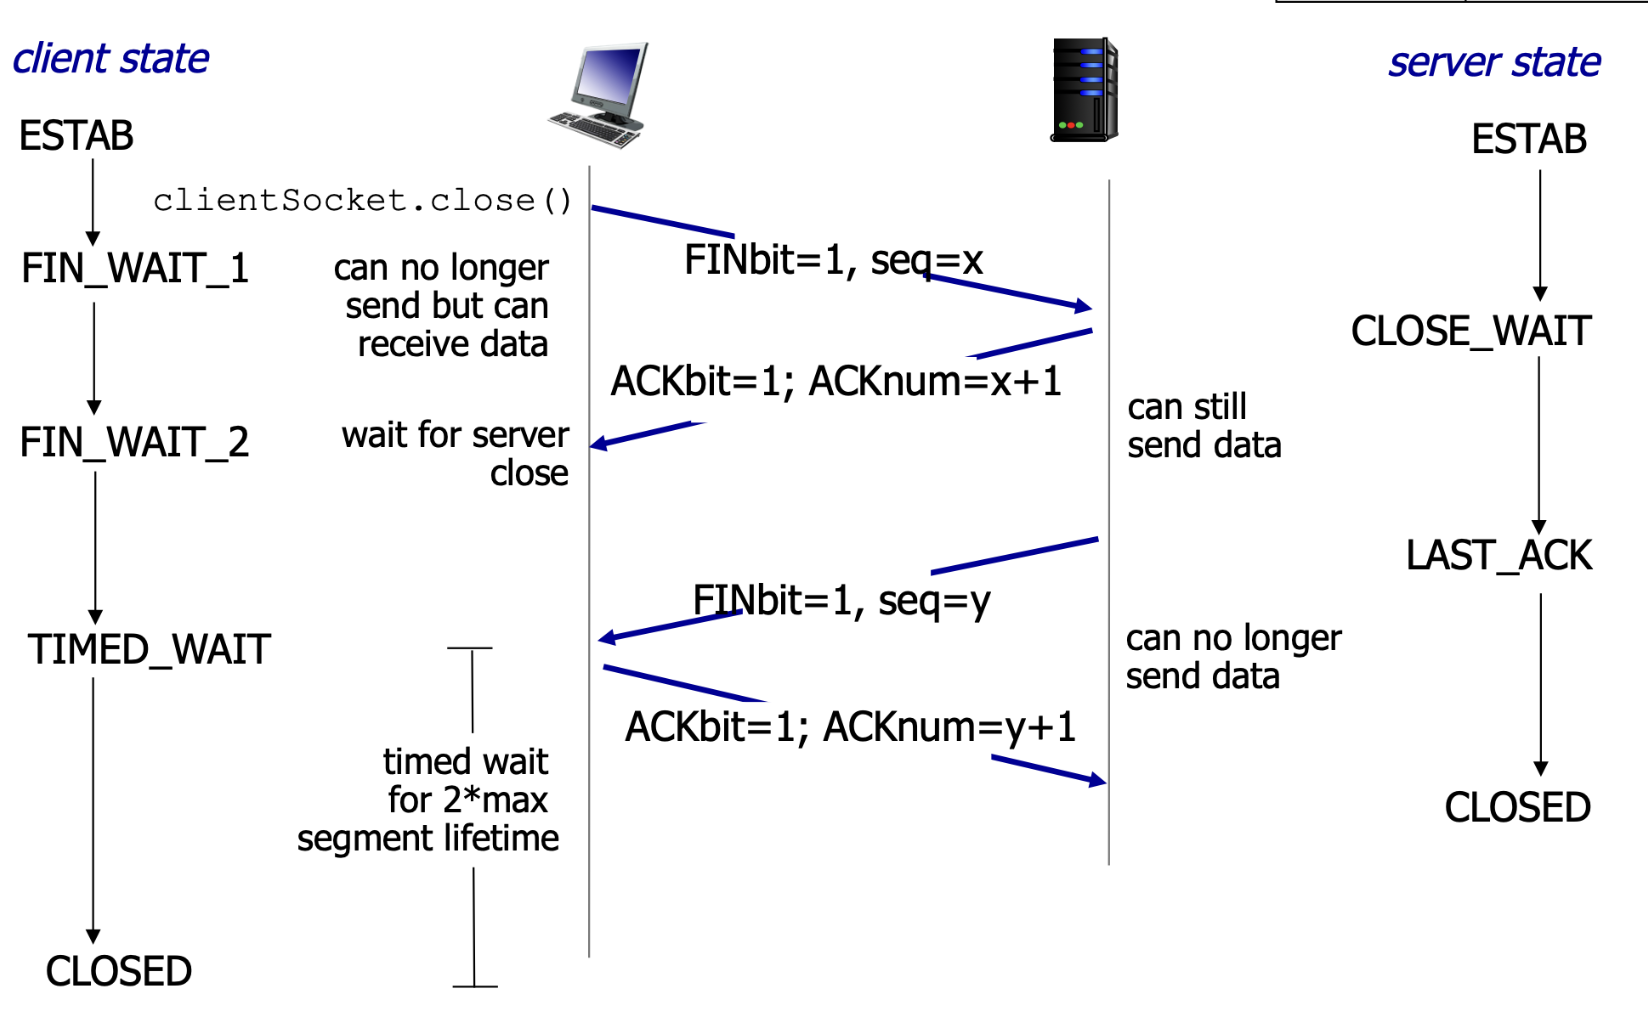
\includegraphics[scale=0.3]{tcp-close}
\\Why TIMED\_WAIT (2*\keyword{MSL}{Maximum segment lifespan})
\begin{itemize}
	\item Guarantee the port has been closed completely
	\item Prevent delayed data segments from being received by other TCP connections
\end{itemize}

\subsection{RDT}
\subsubsection{Features}
\begin{itemize}
	\item Pipelined segments
	\item Cumulative ACKs (like GBN)
	\item Single retransmission timer
	\item Retransmit only missing packets (SR)
\end{itemize}

\subsubsection{Retransmission Scenarios}
Send ACKs every other packet OR after timeout of packet OR receive gapped packet
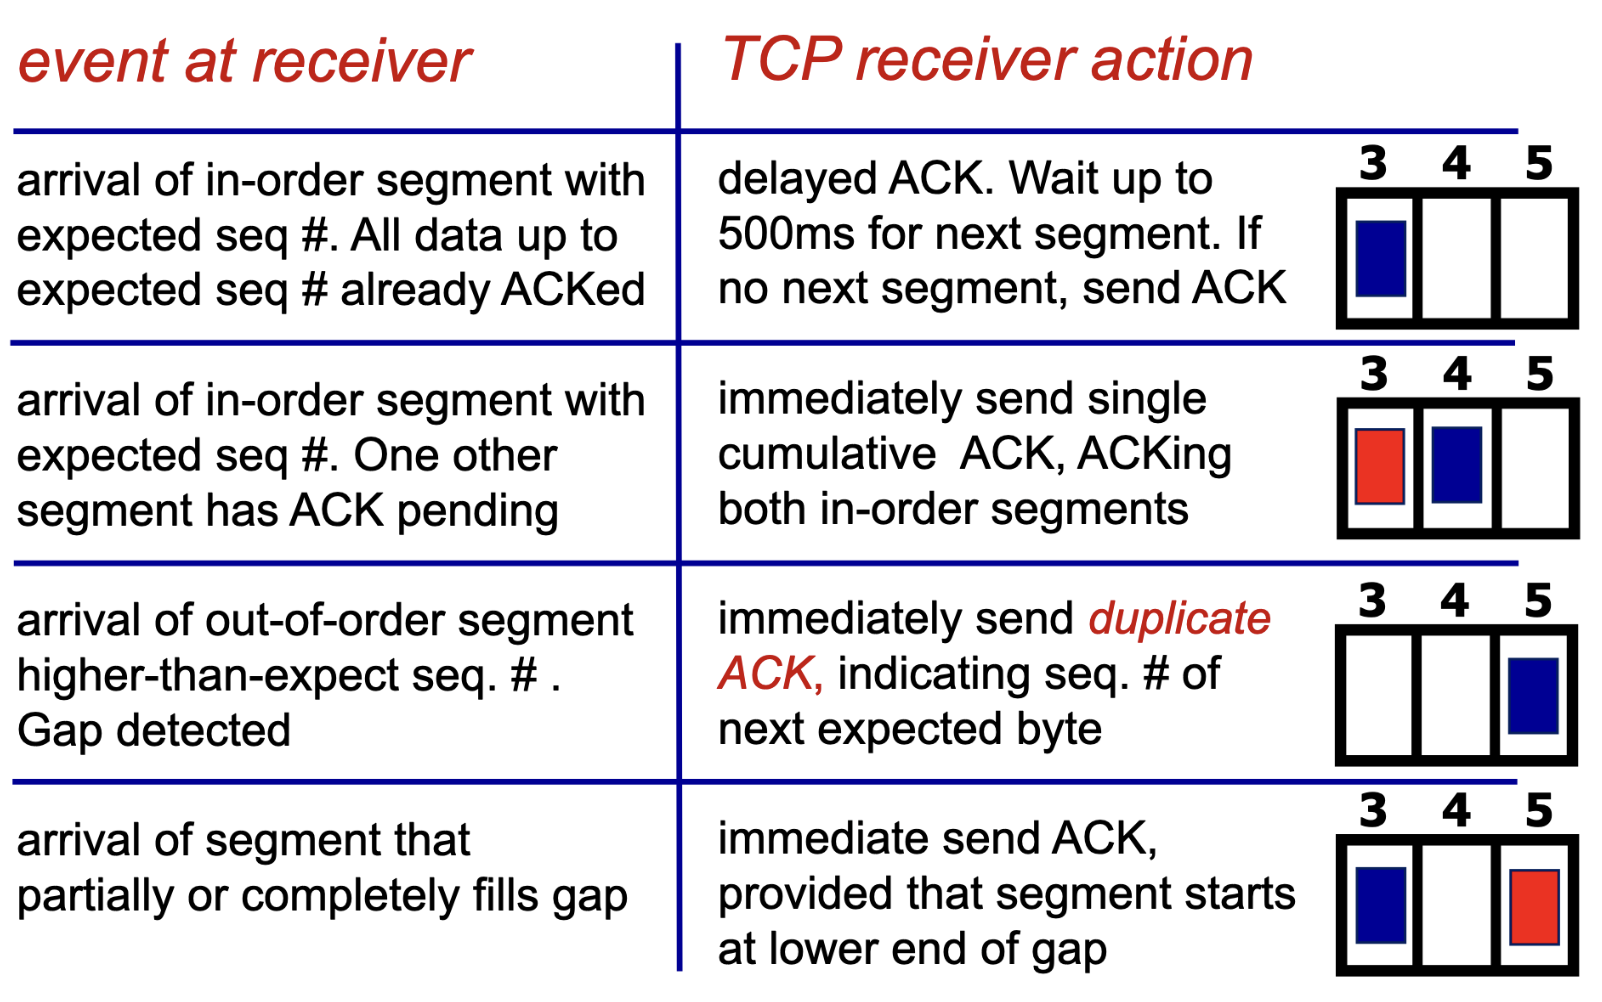
\includegraphics[scale=0.25]{tcp-acks}
\\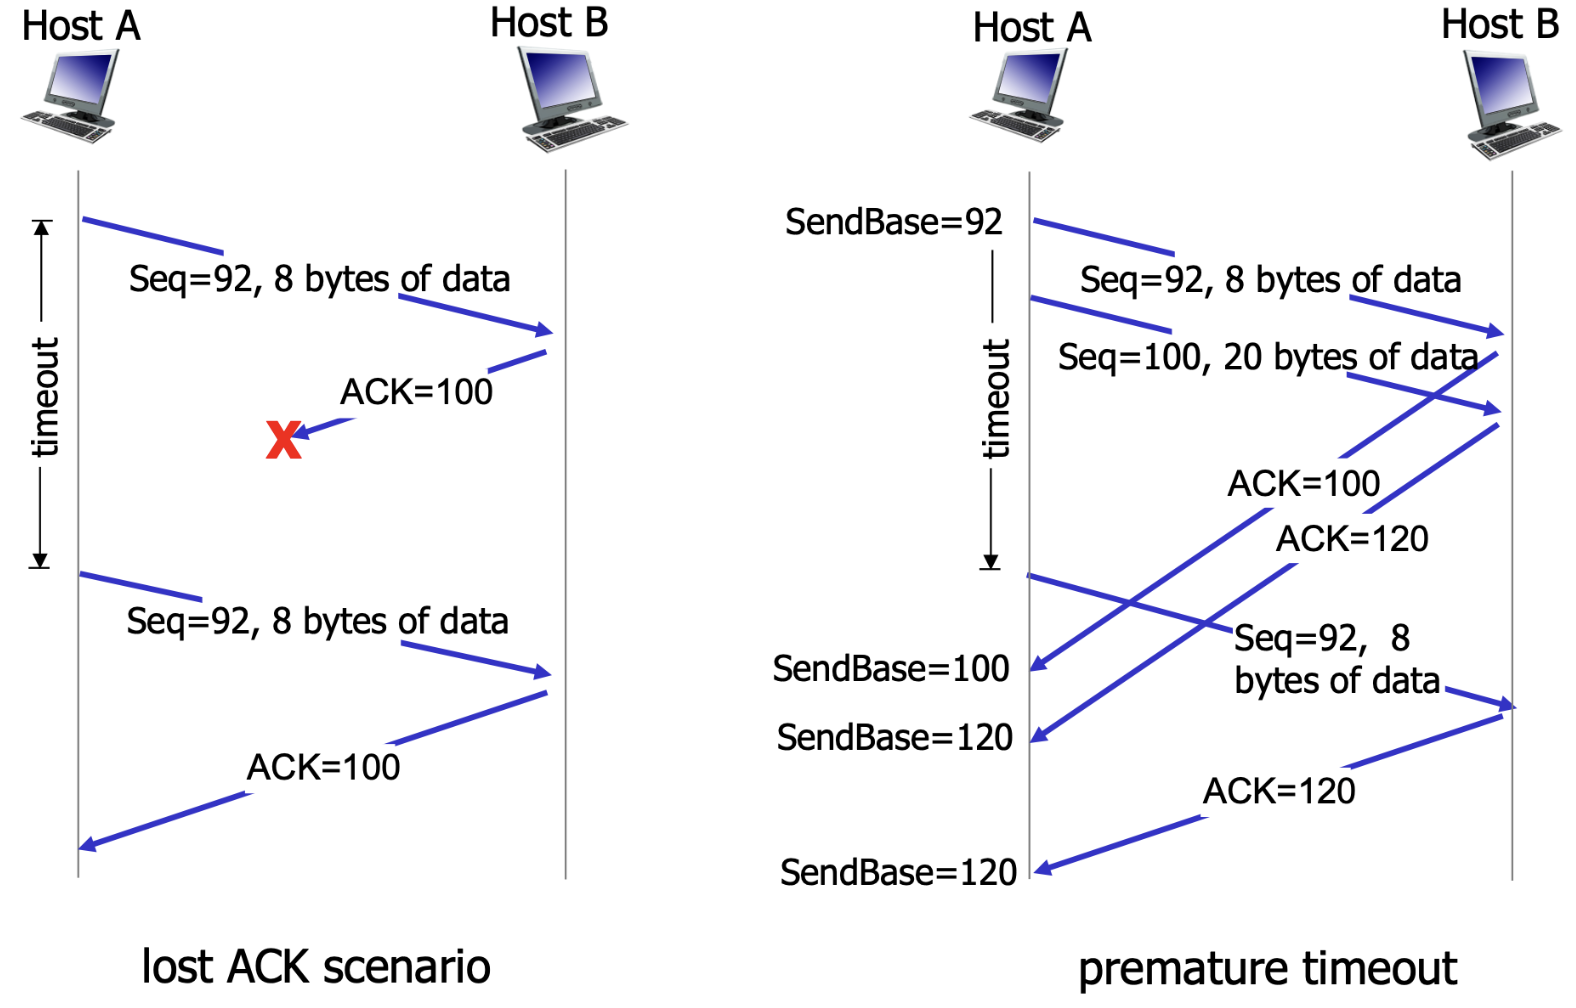
\includegraphics[scale=0.23]{tcp-retransmission1}
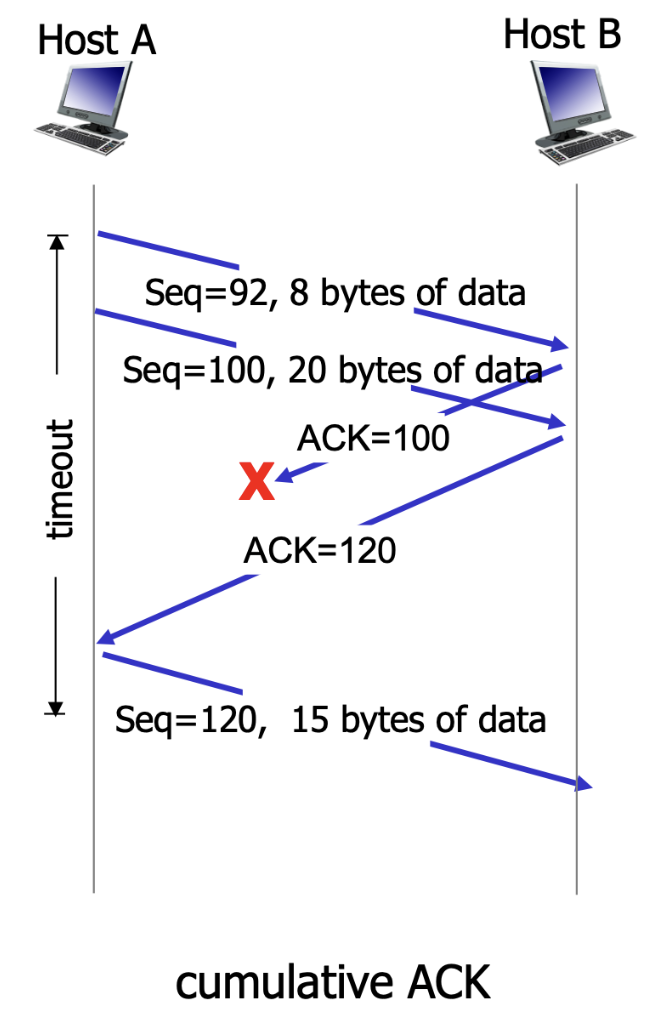
\includegraphics[scale=0.23]{tcp-retransmission2}

\subsubsection{RTT}
\begin{itemize}
	\item Problem: Estimate timeout value for retransmission
	\item Solution: Average recent \keyword{SampleRTT}{Measured time from segment transmission until ACK}
	\item EstimatedRTT = $(1-\alpha) *$ EstimatedRTT + $\alpha*$  SampleRTT
	\begin{itemize}
		\item Exponential weighted moving average
	\end{itemize}
	\item \keyword{DevRTT}{Margin due to deviation from Estimate RTT}
	\begin{itemize}
		\item $(1 - \beta) *$ DevRTT + $\beta *$ (Sample RTT - Estimated RTT)
	\end{itemize}
	\item \keyword{Timeout Interval}{EstimatedRTT + 4 * DevRTT}
	\item $\alpha\approx\frac{1}{8}$, $\beta\approx\frac{1}{4}$
\end{itemize}

\subsubsection{Fast retransmission}
\begin{itemize}
	\item Retransmit unacked segment \textbf{IMMEDIATELY} with \textbf{smallest seq \#} after receiving 4 ACKs for same data
\end{itemize}

\rule{8cm}{1pt}
\section{Midterm tips}
\begin{enumerate}
	\item Bits are b and bytes are B (8 bits = byte)
\end{enumerate}

\rule{8cm}{1pt}

% -----------------------------------------------------------------------
\section{06: IP Addressing}

\subsection{Function}
\begin{enumerate}
	\item \keyword{Forwarding}{Move packets from router input to output}
	\item Routing
	\begin{itemize}
		\item Determine route taken by packets from source to destination
		\item Plan trip from source to destination
	\end{itemize}
\end{enumerate}

\subsection{Planes}
\begin{enumerate}
	\item Data plane
	\begin{itemize}
		\item Local per router function
		\item Determines how datagram forwarded to output port
	\end{itemize}
	\item Control plane
	\begin{itemize}
		\item Network wide logic
		\item Routing algorithms
	\end{itemize}
\end{enumerate}
\subsection{Subnet}
\begin{itemize}
	\item Network formed by directly interconnected host
	\item Internal host can communicate without router
	\item Connect to external networks with router
	\item Same network prefix
	\item Valid subnet masks
	\begin{itemize}
		\item 254, 252, 248, 240, 224, 192, 128
	\end{itemize}
\end{itemize}

\subsubsection{Special subnet}
\begin{itemize}	
	\item Private IP addresses - 10.0.0.0/8, 172.16.0.0/12, 192,168.0.0/16
	\item Loopback address 127.0.0.0/8
	\item Broadcast 255.255.255.255/32
\end{itemize}

\subsubsection{CIDR}
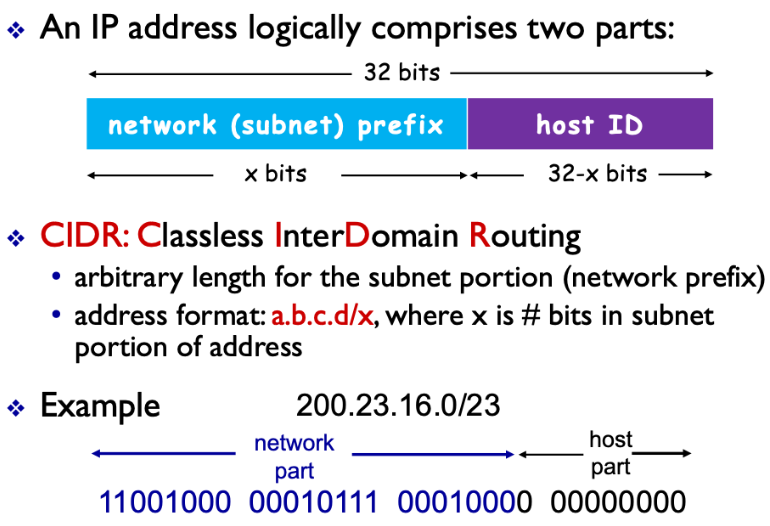
\includegraphics[scale=0.25]{ip-cidr}
\subsubsection{Subnet mask}
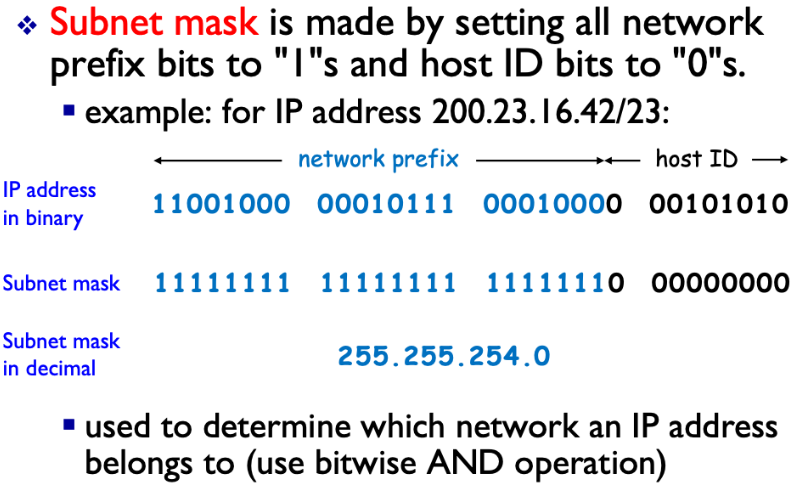
\includegraphics[scale=0.25]{subnet-mask}

\subsubsection{Hierachial addressing}
\keyword{Route aggregation}{Advertise routing information by grouping similar IP addresses}
\\Longest Prefix matching
\begin{tabbing}
	\= Routes to subnet with the greatest subnet portion of CIDR
\end{tabbing}

\subsection{DHCP}
\keyword{Dynamic Host Configuration Protocol}{Lease IP address from network server when joining network}
\begin{itemize}
	\item Runs over UDP , Client \#:68
	\item Router can act as DHCP
	\item Server \#: 67, sends "DHCP ack" and "DHCP offer" 
	\item Client \#: 68, sends "DHCP request" and "DHCP discover" 
\end{itemize}

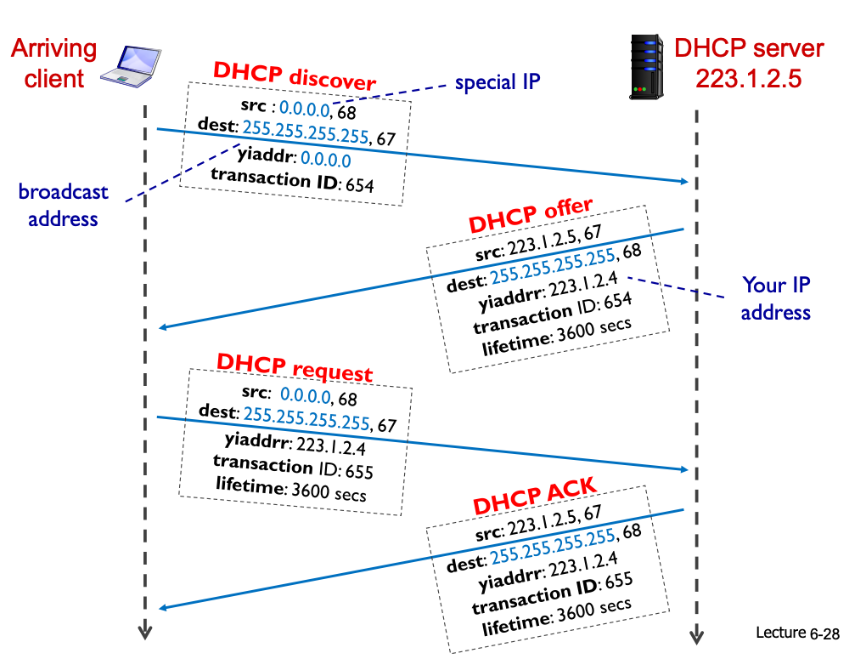
\includegraphics[scale=0.28]{dhcp}
\\What happens when multiple servers in network?
\begin{itemize}
	\item Transaction ID specifies the DHCP connection
\end{itemize}

%--------------------------------------------------------------------------------------------------------------------------------
\section{07. IP (cont)}
\subsection{IP fragmentation}
\keyword{MTU}{Maximum Transfer Unit, maximum amount of data a link-level frame can carry}\\
\keyword{Fragmentation}{Large datagrams that are broken up by routers}
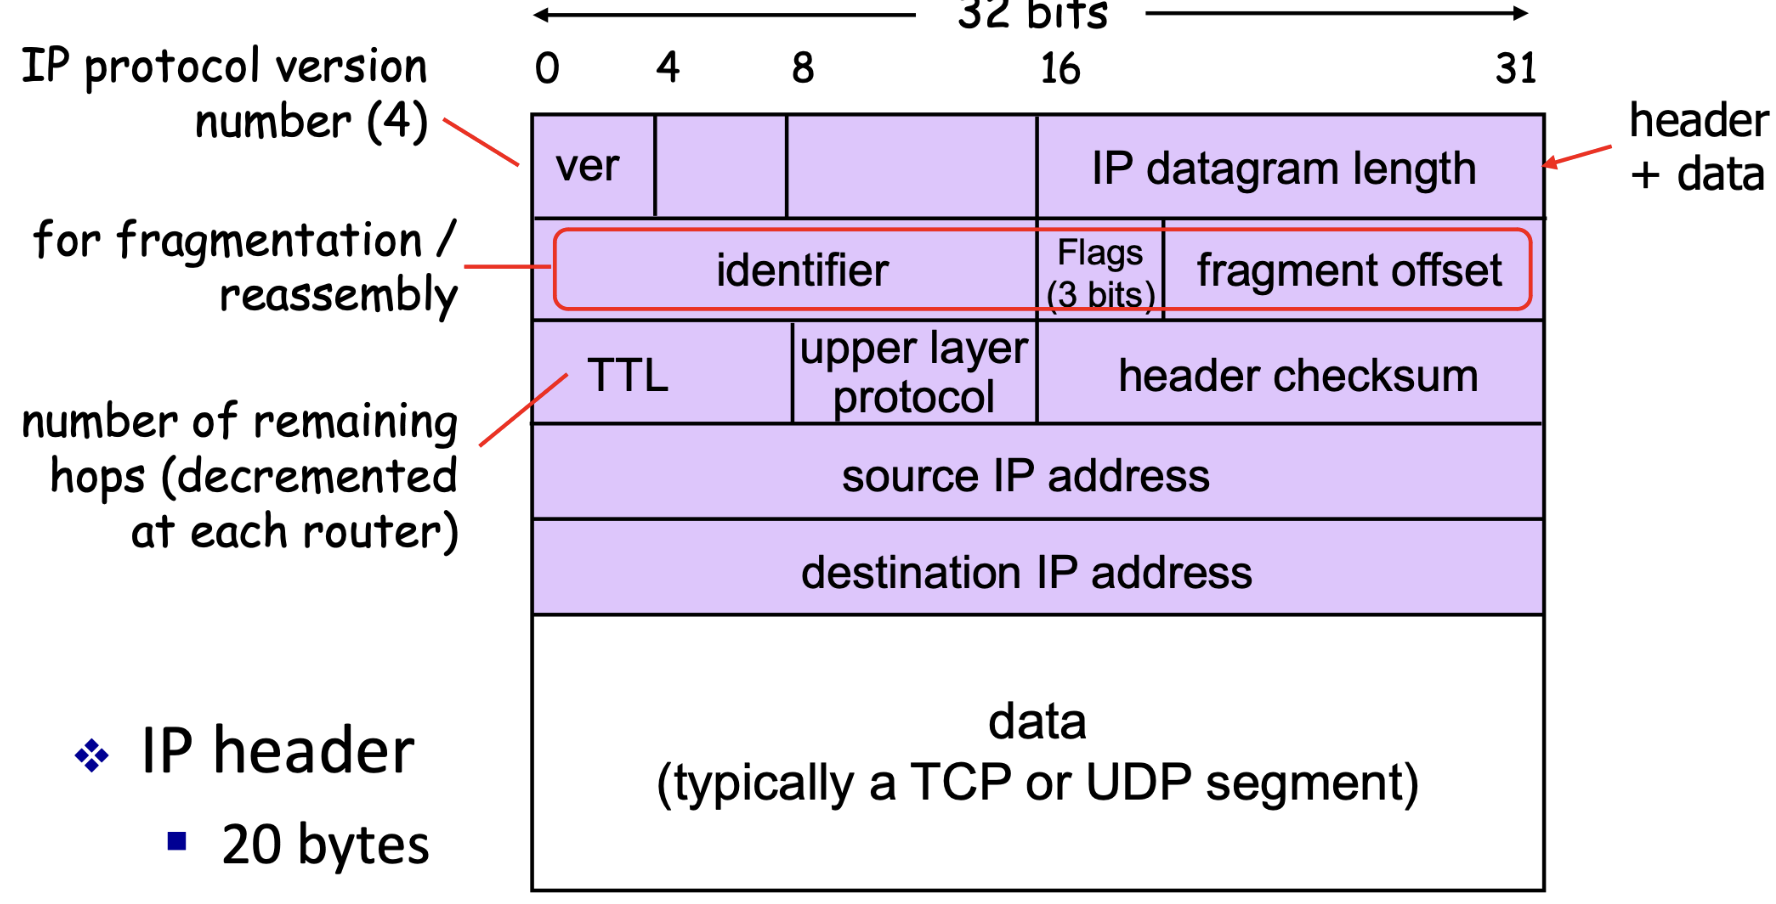
\includegraphics[scale=0.2]{ipv4-datagram-format}
\begin{itemize}
	\item Frag flag = 1 if there are more fragments from same segment, 0 = last fragment
	\item Offset - in units of 8-bytes specifying the offset of fragment wrt beginning of unfragmented IP datagram
\end{itemize}
\textbf{Problem:}\\
Not enough IP addresses to specify all devices
\subsection{Network Address Translation}
Using private IP addresses to map devices within an organisation and enable communication with the internet\\
\begin{itemize}
	\item WAN (Wide area network) vs LAN (Local area network) - private vs public IP address
\end{itemize}
\subsubsection{Implementation}
\begin{itemize}
	\item Routers replace source Ip address, port num of every outgoing datagram to NAT IP address and new port num
	\item Remember (in NAT translation table) the mapping of the source vs NAT info
	\item Replace NAT ip address and port num in destination fields of incoming datagrams with corresponding source IP/port stored in NAT translation table
\end{itemize}

\subsubsection{Motivation}
\begin{itemize}
	\item No need to rent a range of public IP addresses from ISP: just 1 for NAT
	\item Hosts using private IP address can have variable IP addresses without notifying other hosts
	\item Can change ISP without changing addresses of host in LAN
	\item Hosts in Lan are not explicitly addressable and visible by outside (Security)
\end{itemize}

\subsubsection{Challenges}
\begin{itemize}
	\item Difficult to have p2p applications across WANs
\end{itemize}

\subsection{Routing}
Hierachial routing on internet due to size and decentralised administration\\
Goal: Find the least cost to connect 2 hosts through routers
\subsubsection{Intra Autonomous system(AS) routing}
\begin{itemize}
	\item Finds good path between routers within AS
	\item Single admin so no policy decision needed
	\item Performance impt in routing
	\item Protocols - RIP and OSPF
\end{itemize}

\subsubsection{Inter AS routing}
\begin{itemize}
	\item Handles interfaces between AS
	\item Admin wants control over traffic routing
	\item Policy \> performance
	\item Protocol - BGP
\end{itemize}

Cost associated along each link based on various factors
\begin{itemize}
	\item Inversely related to bandwidth
	\item Related to congestion of router
	\item Distance, \$
\end{itemize}

\subsubsection{Distance vector}
Iterative Bellman-Ford computation
\begin{enumerate}
	\item Starting router queries all the neighbours around it
	\item Neighbours could have cached the distance vector to other routers
	\begin{enumerate}
		\item Router can send the table of distance vectors to the new router (routing tables)
	\end{enumerate}
	\item No/incomplete distance vector record: WAit for (change in local link cost or message from neighbour)
	\item Recomputes DV estimates using DV received from neighbour
	\item Notify neighbours if DV to any destination changes
\end{enumerate}

\begin{itemize}
	\item Iterative and asynchronous: local iteration caused by
	\begin{itemize}
		\item Local link cost changes
		\item DV update messages from neighbours
	\end{itemize}
	\item Distributed and self stopping
	\begin{itemize}
		\item Each node notifies neighbours \textbf{only} when DV changes (if necessary)
	\end{itemize}
\end{itemize}

\subsubsection{Link state algorithms}
\begin{itemize}
	\item Periodically braodcasting link costs to each other
	\begin{itemize}
		\item \textbf{All} routers have complete knowledge of topology and link cost
	\end{itemize}
	\item Use Dijkstra algorithm to compute least cost path locally
\end{itemize}

\subsubsection{Routing Information Protocol(RIP)}
\begin{itemize}
	\item Implements DV algorithm
	\item Uses hop count as cost metric
	\item \keyword{Self-repair}{If no updates from router for 3 minutes will assume router fails}
	\item Exchanges routing table every 30s (UDP - 520)
\end{itemize}

\subsection{Internet Control Message Protocol - ICMP}

Used by hosts and routers to communicate network information
\begin{description}
	\item When TTL is 0, packet is discarded and ICMP error message is sent to datagram's source address
	\item[Error reporting]{Unreachable host/network/port/protocol}
	\item[Echo Request]
	\item[Headers]{Starts after IP header carried in IP datagrams}
\end{description}
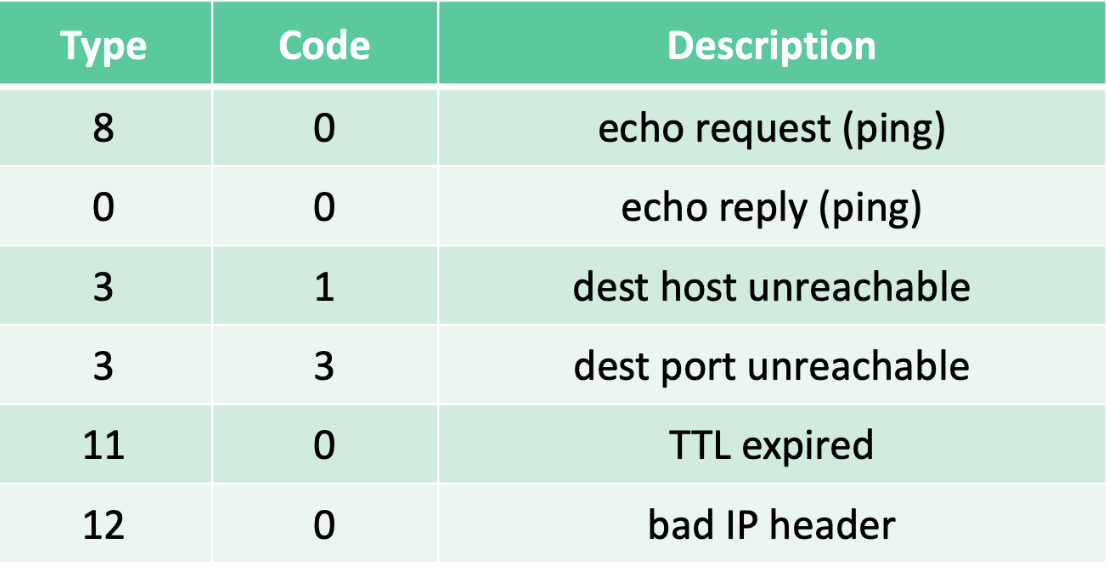
\includegraphics[scale=0.2]{icmp-type-and-code}
\subsubsection{Ping}
\begin{itemize}
	\item Used to echo and test connection between different remote hosts
	\item Format: $XX$ bytes from $client~ip$: icmp\_seq=$X$ ttl=$X$ time=$X$ms
	\item Time == time taken for ping command to execute completely
	\item ttl = number of hops between client and remote host
	\item icmp\_seq = index of the datagrams sent to remote host (ascending order, default 0..6)
\end{itemize}
\subsubsection{Traceroute}
\begin{itemize}
	\item Sends series of small packets with different TTL to display route to get to host
	\item Mechanism
	\begin{itemize}
		\item TTL decrements every hop from initial TTL, X
		\item Once TTL has reached 0, it will immediately reply with ICMP error message, addressed from the current device to the original source
		\item Extract source IP address from the reply to get the device X hops away
	\end{itemize}
\end{itemize}

\section{08. Link layer}
\subsection{Motivation}
\begin{itemize}
	\item Sending data between N nodes via cable
	\begin{itemize}
		\item Interconnect the N nodes via broadcast link
		\item Every link has to be addressed
		\item Define protocol so address to node on shared link (who speaks when and for how long)
		\item Need to handle errors (Detection and reliability)
	\end{itemize}
	\item \keyword{Communication channel}{Transmission medium of data signals}
	\item Link layer sends frames transmitted between \textbf{physically adjacent} nodes over single link
\end{itemize}
\subsection{Services}
\begin{description}
	\item[Framing]{Encapsulate IP datagram into frame by adding header and trailer}
	\item[Link Access Control]{Coordinate which nodes send frames at specific time}
	\item[Error detection]{Errors caused by signal attenuation or noise detected by receiver that signals sender for retransmission}
	\item[Error correction]{Identifies and correct bit errors without transmission}
\end{description}
\subsubsection{Devices}
\begin{itemize}
	\item Implemented in NIC (network interface card) or on a chip (ethernet card/wifi adapter)
	\item Adapters are semi-autonomous and implements link and physical layer
\end{itemize}
\subsection{Error Detection and correction}
\subsubsection{Schemes}
\begin{itemize}
	\item Checksum (used in TCP/UDP/IP)
	\item Parity checking
	\begin{itemize}
		\item Maintains a parity bit that value dependent on total number of 1s (where d+1 bit is even - even parity scheme)
		\item Detect odd number of single bit errors
		\item Probability of multiple bit errors is low (if errors are independent)
		\item IRL errors are clustered so P(undetected errors) $\approx 50\%$
		\item Can be made 2-D where d bits divided into i rows and columns
		\item Parity bit along each row and column
		\item Detects and corrects bit errors in data by comparing horizontally and vertically for errors
	\end{itemize}
	\item Cyclic redundancy check (CRC)
	\begin{enumerate}
		\item Decide generator G and number of bits to append, R
		\item For every info sent, append R bits of 9 to the back of the data, X
		\item Data sent is the largest value less than X divisible by G
		\item At receiver, data has error when it is indivisible by G
	\end{enumerate}
	\begin{itemize}
		\item Easy to implement (Appending 0s and modulo 2 arithmetic xor)
		\\
		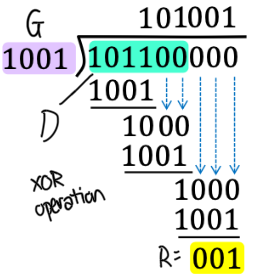
\includegraphics[scale=0.24]{CRC-example}
		\item Powerful error detection (detects all errors less than r+1 bit + $P(1-0.5^{r})$ error $>$ r bits
		\item AKA polynomial code
	\end{itemize}
\end{itemize}
\subsection{Multiple access links \& protocol}
\subsubsection{Types of links}
\begin{itemize}
	\item Point-to-point
	\begin{itemize}
		\item Sender-receiver connected by dedicated link (no need multiple access control)
		\item Point-to-point protocol, serial line internet protocol
	\end{itemize}
	\item Broadcast link (shared medium)
	\begin{itemize}
		\item Multiple nodes in a shared broadcast channel
		\item Channel broadcast frames to all nodes in the network
		\item Wifi, satellite, bus ethernet
	\end{itemize}
\end{itemize}
\subsubsection{Motivation}
\begin{itemize}
	\item Collision happens when nodes receives two or more signals concurrently
	\item Need protocol to decide who, when and how long nodes get to communicate
\end{itemize}
\subsection{Transmission algorithms}
\subsubsection{Goals}
\begin{description}
	\item[Collision free]
	\item[Efficient]{Node can send at rate R(max transmission rate)}
	\item[Fairness]{When M nodes want to transmit, each sends at an average rate R/M}
	\item[Decentralised]{No dedicated driver/node to coordinate transmission}
\end{description}
\textbf{Channel partitioning}
\subsubsection{Time division multiple access (TDMA)}
\begin{itemize}
	\item Access channels in fixed length time slots each round
	\item Not very efficient as unused slots go idle (max throughput is R/N)
	\item Collision free, fair and decentralised\\
	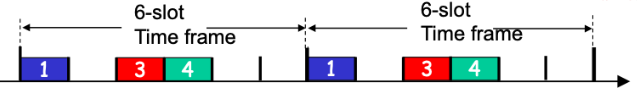
\includegraphics[scale=0.25]{tdma-rounds}
\end{itemize}
\subsubsection{Frequency division multiple access (FDMA)}
\begin{itemize}
	\item Channel spectrum divided into frequency bands
	\item Node assigned to fixed band
	\item Same pros cons as TDMA
\end{itemize}
\textbf{Take turn}
\subsubsection{Polling protocol}
\begin{itemize}
	\item Taking turn protocol that requires one node to be designated master node
	\item Master node polls each node in round robin to assign usage
	\item High efficiency, collision free, fair (proper algo for master node) but not decentralised
\end{itemize}
\subsubsection{Token passing}
\begin{itemize}
	\item Token passed from one node to next sequentially
	\item Holds token $\iff$ want to transmit frames else forward token to next node
	\item Collision free, high efficiency (negligible overhead from token passing), fair and decentralised
	\item Might be disruptive (frame loss, system bugs) or node failure
\end{itemize}
\textbf{Random access}
\subsubsection{Slotted ALOHA}
\begin{itemize}
	\item Split time into slots of equal size(synchronised among all nodes)
	\item Nodes transmit at full channel transmission rate \textbf{ONLY} at the beginning of a slot (randomly)
	\item Have collisions and partially efficient (maximum efficiency at 37\% because collision and empty slots)
	\item Perfectly fair and decentralised
\end{itemize}
\subsubsection{Unslotted ALOHA}
\begin{itemize}
	\item No time slots/synchronisation and transmit entire frame immediately
	\item Retransmit frames with probability p everytime there is collision until success
	\item Chance of collisions increase (max efficiency at 18\%)
\end{itemize}
\subsubsection{Carrier Sense Multiple Access (CSMA)}
\begin{itemize}
	\item Node decision to transmit is dependent of activity of other nodes attached to channel
	\item Node detects if other node is transmitting before transmission (defers transmission when channel is busy)
	\item Collisions may still occur due to propagation delay (does not detect other nodes transmissions immediately)
\end{itemize}
\subsubsection{CSMA/Collision Detection}
\begin{itemize}
	\item Abort transmission immediately when collision detected
	\item Frame is retransmitted after random delay
	\item \keyword{Backoff algorithm}{Adapts retransmission attempts to estimated current load}
	\begin{itemize}
		\item More collisions implies heavier load -\> increase back-off interval with more collisions
		\item Binary exponential backoff (Probability of resending = $2^{-m-1}$ after m collisions)
	\end{itemize}
	\item Enforce minimum frame size to ensure collision is detected (account for propagation delay)
	\item Not collision free but efficient, fair and decentralised
\end{itemize}

\section{09. Link layer LAN}
\subsection{Media Access Control (MAC)}
\begin{itemize}
	\item Used to send and receive link layer frames
	\item Found on every NIC adapter
	\item If dest MAC == nic mac, extract datagram and pass to protocol stack | else discard frame without interruption
	\item 48 bits burnt in NIC ROM (read only memory) administered by IEEE
	\item First 3 bytes specify vendor of adapter
	\item Can run ifconfig $<$interface$>$ on unix systems to get the information
\end{itemize}
\keyword{Local Area Network (LAN)}{Network that interconnects computers within geographical area}	
\subsection{Ethernet}
\begin{itemize}
	\item Dominant wired Lan technology
	\item 802.3 Standards with different band speeds and physical layer media
	\item Frame Structure\\
	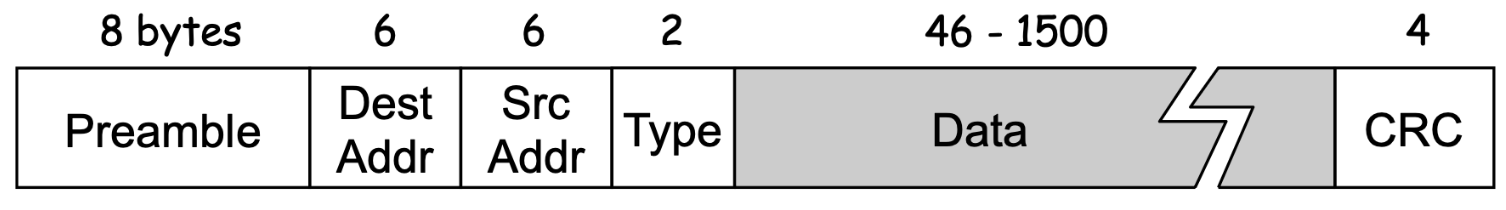
\includegraphics[scale=0.2]{ethernet-frame-structure}
	\item Note that hosts can use other network-layer protocol besides IP (Type field)
	\item Preamble used to synchronise receiver and sender clock rates
	\begin{itemize}
		\item 7 bytes of 10101010 (0xAA)
		\item 1 byte of 10101011 (0xAB) (start of frame)
	\end{itemize}
\end{itemize}
\subsubsection{Data delivery service}
\begin{itemize}
	\item Unreliable (no ACK or NAK to sender NIC)
	\begin{itemize}
		\item Data in dropped frames will only be recovered if initial sender uses higher layer RDT
	\end{itemize}
	\item Uses CSMA/CD with binary (exponential) backoff
\end{itemize}
\subsubsection{Topology}
\begin{itemize}
	\item \textbf{Bus topology} popular till mid 90s (broadcast Lan)
	\item Cons:
	\begin{itemize}
		\item Backbone cable (network fails if damaged)
		\item Difficult to troubleshoot problems
		\item Slow and not ideal for large networks
	\end{itemize}
	\item \textbf{Star} prevelant today 
	\item \keyword{Hubs}{physical layer device}
	\begin{itemize}
		\item Cheap with easy maintenance
		\item Slow and may not be ideal for larger networks (Collision)
	\end{itemize}
	\item \keyword{Switch}{Link layer device with no collisions}
	\begin{itemize}
		\item Store and forward packet switch
	\end{itemize}
\end{itemize}
\subsection{Switch}
\subsubsection{Function}
\begin{itemize}
	\item Examine incoming frame Mac address 
	\item Selectively store and forward frame to one or more outgoing links (CSMA/CD)
	\item Transparent (hosts unaware of switches)
	\item Plug and play - no need configuration
\end{itemize}
\subsubsection{Mechanism}
\begin{itemize}
	\item Nodes have dedicated direct connection to switch
	\item Ethernet protocol used without collision due to switching
	\item Maintains switching forwarding table for \keyword{selective forwarding}{only sending frames to the correct interfaces}
	\begin{itemize}
		\item Format \textit{Mac address of host, interface to reach host, TTL}
	\end{itemize}
	\item \keyword{Self learning}{Records sender/location pair in switch table everytime frames are received}
\end{itemize}
\begin{enumerate}
	\item Record incoming link, Mac address of sending host
	\item Index switch table using Mac destination address
	\item If entry found for destination,
	\begin{enumerate}
		\item if destination is in the same segment as source ? drop : forward frame on destination interface		
	\end{enumerate}
	\item else flood - forward on all interface except arriving interface
\end{enumerate}
\subsubsection{vs Router}
\begin{itemize}
	\item Checks MAC vs IP address
	\item Both store and forward
	\item Forward frame to link/broadcast vs Route computation
\end{itemize}
\subsection{Address Resolution Protocol}
\begin{itemize}
	\item Maps IP address and MAC address of nodes in the same subnet
	\item TTL - time until address mapping will be forgotten
\end{itemize}
Resolution when in same subnet
\begin{enumerate}
	\item Broadcast ARP query with B's ip as dest
	\begin{itemize}
		\item Dest mac == FF-FF-FF-FF-FF-FF
		\item All nodes in same subnet receives but only B replies
	\end{itemize}
	\item B replies to A with its MAC address
	\item A cache B's IP-Mac address mapping in ARP table until TTL
\end{enumerate}
Different subnet
\begin{enumerate}
	\item Sends packet with correct MAC and IP but no response because different subnet
	\item Resends packet with dest MAC == router MAC
	\item Datagram removed passed to IP where routing calculations determine the subnet it is in (at router)
	\item Router attaches dest MAC address again or use ARP with correct IPs
	\item Receiver receives the information
\end{enumerate}
\subsection{IP vs MAC address}
\begin{itemize}
	\item 32 bits vs 48 bits
	\item Network-layer address used to move datagrams from src to dest vs link layer address to move frames over each link
	\item Dynamic assignment;hierachial vs permanent
\end{itemize}

\end{multicols*}
\end{document}
